\documentclass[sigconf,10pt]{acmart}
\settopmatter{printacmref=false}

%\usepackage[show]{notes}

\pdfpagewidth=8.5in
\pdfpageheight=11in

%\usepackage[T1]{fontenc}
\renewcommand{\rmdefault}{ptm}
%\usepackage{mtpro2}
\usepackage{varwidth,times}
\usepackage{amsmath}
\usepackage{amsthm}
\usepackage{amssymb}
\usepackage{amsfonts}
\usepackage{epsfig}
\usepackage{graphicx}
% \usepackage{subfigure} %OBSOLETE
\usepackage{url}
\usepackage[bottom]{footmisc}
\usepackage{balance}
\usepackage{mathtools}

% \usepackage{algorithm}% http://ctan.org/pkg/algorithms
% \usepackage{algpseudocode}%http://ctan.org/pkg/algorithmicx
% % \usepackage[linesnumbered,ruled]{algorithm2e}
% \algrenewcommand\textproc{}% Used to be \textsc
% \renewcommand{\algorithmicrequire}{\textbf{Input:}}
% \renewcommand{\algorithmicensure}{\textbf{Output:}}
% \usepackage{calc} % for \widthof
% \algrenewcommand\algorithmicensure{%
%   \makebox[\widthof{\textbf{Require:}}][l]{\textbf{Ensure:}}} 

% \usepackage[noend]{algorithmic}
% \usepackage{algorithm2e}
\usepackage{amsmath}
\usepackage{mathtools}
\usepackage[ruled, vlined, linesnumbered]{algorithm2e}
% \SetVlineSkip{0pt}      
\let\oldnl\nl% Store \nl in \oldnl
\newcommand{\nonl}{\renewcommand{\nl}{\let\nl\oldnl}}
% Remove line number for one line

\usepackage{multirow}
\usepackage{xspace}
%\usepackage{latexsym}
\usepackage{xcolor}
%\usepackage{multirow}
%\usepackage{times}
%\usepackage{cite}
\usepackage{tikz}
% \usepackage[singlelinecheck=off]{caption}
\usepackage{caption}
\usepackage{subcaption}
\captionsetup{justification=raggedright,textfont=normalfont,singlelinecheck=false}
\captionsetup[subfigure]{labelfont=normalfont,textfont=normalfont,singlelinecheck=on,justification=raggedright, skip=15pt}
% \captionsetup[subfigure]{skip=15pt} % global setting for subfigure

\DeclareCaptionType{copyrightbox}
%\usepackage{url}
%\usepackage{justification=justified,singlelinecheck=false}{caption}
%\pagestyle{empty}


%                  General Macros
%\theoremstyle{plain}
\newtheorem{thrm}{Theorem}
%\newtheorem{proposition}{Proposition}
\newtheorem{property}{Property}
%\newtheorem{corollary}{Corollary}
\newtheorem{lma}{Lemma}
\newtheorem{claim}{Claim}
%\newtheorem{conjecture}{Conjecture}
\newtheorem{defn}{Definition}
\newtheorem{remark}{Remark}
\newtheorem{exple}{Example}
\newtheorem{problem}{Problem}
\newtheorem{observation}{Observation}

%\newtheorem{proofproposition}{Proof of Proposition}
%\newtheorem{proofcorollary}{Proof of Corollary}
%\newtheorem{prooftheorem}{Proof of Theorem}
%\newtheorem{prooflemma}{Proof of Lemma}

%                   Para
\newcommand{\spara}[1]{\smallskip\noindent{\bf #1}}
\newcommand{\mpara}[1]{\medskip\noindent{\bf #1}}
\newcommand{\para}[1]{\noindent{\bf #1}}


%% tight spacing in item lists
\newcommand{\squishlist}{
 \begin{list}{$\bullet$}
  {  \setlength{\itemsep}{0pt}
     \setlength{\parsep}{3pt}
     \setlength{\topsep}{3pt}
     \setlength{\partopsep}{0pt}
     \setlength{\leftmargin}{2em}
     \setlength{\labelwidth}{1.5em}
     \setlength{\labelsep}{0.5em}
} }
\newcommand{\squishlisttight}{
 \begin{list}{$\bullet$}
  { \setlength{\itemsep}{0pt}
    \setlength{\parsep}{0pt}
    \setlength{\topsep}{0pt}
    \setlength{\partopsep}{0pt}
    \setlength{\leftmargin}{2em}
    \setlength{\labelwidth}{1.5em}
    \setlength{\labelsep}{0.5em}
} }

\newcommand{\squishdesc}{
 \begin{list}{}
  {  \setlength{\itemsep}{0pt}
     \setlength{\parsep}{3pt}
     \setlength{\topsep}{3pt}
     \setlength{\partopsep}{0pt}
     \setlength{\leftmargin}{1em}
     \setlength{\labelwidth}{1.5em}
     \setlength{\labelsep}{0.5em}
} }

\newcommand{\squishend}{
  \end{list}
}


%%%%%%%%%%%%%%%%%%%%%%%%%%%%%%%%%%%%%%%%%%%%%%%%%%%%%%%%%%%%%%%%%%%%%%%%%%%%%%
% ALGORITHMS
%%%%%%%%%%%%%%%%%%%%%%%%%%%%%%%%%%%%%%%%%%%%%%%%%%%%%%%%%%%%%%%%%%%%%%%%%%%%%%%
\newcommand{\SELECT}{\mbox{{\bf select}}\ }
\newcommand{\FROM}{\mbox{{\bf from}\ }}
\newcommand{\WHERE}{\mbox{\bf where}\ }
\newcommand{\SUM}{\mbox{{\bf sum}}\ }
\newcommand{\GROUPBY}{\mbox{{\bf group by}}\ }
\newcommand{\HAVING}{\mbox{{\bf having}}\ }
\newcommand{\CASE}{\mbox{{\bf case}}\ }
\newcommand{\END}{\mbox{{\bf end}}\ }
\newcommand{\WHEN}{\mbox{{\bf when}}\ }
\newcommand{\EXISTS}{\mbox{{\bf exists}}\ }
\newcommand{\COUNT}{\mbox{\kw{count}}}
\newcommand{\INSERTINTO}{\mbox{{\bf insert into}}\ }
\newcommand{\Insert}{\mbox{{\bf insert}}\ }
\newcommand{\UPDATE}{\mbox{{\bf update}}\ }
\newcommand{\SET}{\mbox{{\bf set}}\ }
\newcommand{\IN}{\mbox{{\bf in}}\ }
\newcommand{\If}{\mbox{\bf if}\ }
\newcommand{\Let}{\mbox{\bf let}\ }
\newcommand{\Call}{\mbox{\bf call}\ }
\newcommand{\Then}{\mbox{\bf then}\ }
\newcommand{\To}{\mbox{\bf to}\ }
\newcommand{\EndWhile}{\mbox{\bf endwhile}\ }
\newcommand{\EndFor}{\mbox{\bf endfor}\ }
\newcommand{\EndIf}{\mbox{\bf endif}\ }
\newcommand{\Else}{\mbox{\bf else}\ }
\newcommand{\ElseIf}{\mbox{\bf elseif}\ }
\newcommand{\While}{\mbox{\bf while}\ }
\newcommand{\Begin}{\mbox{\bf begin}\ }
\newcommand{\End}{\mbox{\bf end}\ }
\newcommand{\Do}{\mbox{\bf do}\ }
\newcommand{\Downto}{\mbox{\bf downto}\ }
\newcommand{\Repeat}{\mbox{\bf repeat}\ }
\newcommand{\Until}{\mbox{\bf until}\ }
\newcommand{\For}{\mbox{\bf for}\ }
\newcommand{\Each}{\mbox{\bf each}\ }
\newcommand{\ForEach}{\mbox{\bf for each}\ }
\newcommand{\goto}{\mbox{\bf go to}\ }
\newcommand{\Or}{\mbox{\bf or}\ }
\renewcommand{\And}{\mbox{\bf and}\ }
\newcommand{\Not}{\mbox{\bf not}\ }
\newcommand{\Break}{\mbox{\bf break}\ }
\newcommand{\Continue}{\mbox{\bf continue}\ }
\newcommand{\Return}{\mbox{\bf return}\ }
\newcommand{\Case}{\mbox{\bf case}\ }
\newcommand{\Of}{\mbox{\bf of}\ }
\newcommand{\push}{\mbox{\bf push}\ }
\newcommand{\pop}{\mbox{\bf pop}\ }
\newcommand{\EndCase}{\mbox{\bf end-case}\ }
\newcommand{\NIL}{\mbox{\em nil}}
\newcommand{\False}{\mbox{\em false}}
\newcommand{\True}{\mbox{\em true}}
\newcommand{\algAND}{{\sc and}\xspace}
%\newcommand{\OR}{{\sc or}\xspace}
%\newcommand{\NOT}{{\sc not}\xspace}

\newcommand{\eat}[1]{}
\newcommand{\entity}[1]{\textsf{\scriptsize #1}}
\newcommand{\ie}{i.e.,\xspace}
\newcommand{\eg}{e.g.,\xspace}
\newcommand{\wrt}{w.r.t.\xspace}
\newcommand{\aka}{a.k.a.\xspace}
\newcommand{\kwlog}{\emph{w.l.o.g.}\xspace}
\newcommand{\NP}{\ensuremath{\mathbf{NP}}\xspace}
\newcommand{\sharpP}{\ensuremath{\mathbf{\#P}}\xspace}
\newcommand{\kw}[1]{{\ensuremath {\mathsf{#1}}}\xspace}

\newcommand{\stitle}[1]{\vspace{1.5ex}\noindent{\bf #1}}
\newcommand{\etitle}[1]{\vspace{0.8ex}\noindent{\em #1}}
\newcommand{\blds}[1]{\mbox{\scriptsize \boldmath $#1$}}
\newcommand{\myhrule}{\rule[.5pt]{\hsize}{.5pt}}
\newcommand{\mat}[2]{{\begin{tabbing}\hspace{#1}\=\+\kill #2\end{tabbing}}}
\newcommand{\sstab}{\rule{0pt}{8pt}\\[-2.4ex]}
\newcounter{ccc}
\newcommand{\bcc}{\setcounter{ccc}{1}\theccc.}
\newcommand{\icc}{\addtocounter{ccc}{1}\theccc.}


%macros AK
\newcommand{\planar}{\textsf{Planar}}
\DeclareMathOperator*{\argmin}{arg\,min}
\DeclareMathOperator*{\argmax}{arg\,max}
\newcommand{\bigO}{\mathcal{O}}
\newcommand{\omegatilde}{{\tilde{\Omega}}}


\newcommand{\Sm}{\textsf{Small}}
\newcommand{\SI}{\text{SI}}
\newcommand{\LI}{\text{LI}}
\newcommand{\II}{\text{II}}
\newcommand{\I}{\text{I}}
\newcommand{\sign}{\textsf{sign}}
\newcommand{\Lg}{\textsf{Large}}
\newcommand{\Threshold}{\textsf{Threshold}}
\newcommand{\Stretch}{\textsf{Stretch}}
\newcommand{\LBS}{\textsf{LBS}} 


\pagenumbering{arabic}

\copyrightyear{2020}
\acmYear{2020}
\setcopyright{acmcopyright}
\acmConference[SIGMOD '20]{ACM SIGMOD '20: ACM International Conference on Management of Data}{June 14--19, 2020}{Portland, Oregon, USA}
\acmPrice{15.00}
\acmDOI{10.1145/1122445.1122456}
\acmISBN{978-1-4503-9999-9/18/06}

\begin{document}

\title{Mining Top-$k$ Correlated Subgraphs in a Large Graph}

\author{ACM SIGMOD Submission ID XXX}

%\author{Arijit Khan} \affiliation{\institution{Nanyang Technological
%University}
%}
%\email{arijit.khan@ntu.edu.sg}
%
%\author{Arneish Prateek} \affiliation{\institution{Indian Institute of
%Technology Delhi, India}
%}
%\email{ch1140786@iitd.ac.in}
%
%\author{Sayan Ranu} \affiliation{\institution{Indian Institute of Technology
%Delhi, India}
%}
%\email{sayanranu@iitd.ac.in}
%
%\author{Akshit Goyal} \affiliation{\institution{Indian Institute of Technology
%Delhi, India}
%}
%\email{cs5140278@iitd.ac.in}


\vspace{-4mm}
\begin{abstract}
Mining of correlated patterns, that represent an important class of
regularities, has become increasingly important in data management and
analytics. Surprisingly, the problem of correlated subgraphs mining from a
single, large graph has received little attention. We investigate a novel and
critical graph mining problem, called correlated subgraphs mining, which is
defined as a pair of subgraph patterns that frequently co-occur in proximity
within a single graph.

Correlated subgraphs are different from frequent subgraphs due to the
flexibility in which the constituent subgraph instances are connected, thus the
existing frequent subgraphs mining algorithms cannot be directly applied.
Furthermore, correlation computation between two subgraph patterns require
enumerating and finding distances between every pair of subgraph instances of
both these patterns --- which are both memory intensive and computationally
demanding. 

To this end, we design a novel, single-step, best-first exploration algorithm to
detect correlated subgraph patterns: To further improve the efficiency, we
develop a top-$k$ pruning strategy, while to reduce the memory footprints, we
develop a compressed data structure, called $\mathcal{R}$eplica that stores all
instances of a subgraph pattern. Our empirical results show that the proposed
algorithm not only finds interesting correlations, but also achieves good
performance for finding correlated subgraphs in large graphs.
\end{abstract}

\maketitle

\chapter{Introduction}
\label{sec:intro}

% \eat{
Graphs are a ubiquitous model to represent objects and their complex relations, including protein interaction and genomic graphs in biology,
chemical compound structures in chemistry, food webs and microbial taxa communities in ecology, call graphs in program flow analysis,
social networks in social science, Web graphs, as well as XML documents in e-commerce, government and medical records \cite{SH12}.
Efficient mining of hidden patterns play an important role in developing data-driven methodologies for analyzing the graphs
resulting from such datasets.

Research on graph mining has emerged as one of the hottest topics in recent years due to its wide applications in a variety of fields including
drug discovery \cite{KK01,NK05,YH02}, molecular activity prediction \cite{JYW10,TCG09},
predicting disease susceptibility from gene expression data \cite{RHS13,DI11}, software bug localization \cite{CLZWY09},
clustering and classification of graphs \cite{DKWK05,YCHY08}, anomaly detection \cite{ATK15}, and graph anonymization \cite{LAW11}.
Several variants of graph pattern mining have been proposed,
such as frequent subgraphs \cite{YH02,EASK14}, approximate subgraphs \cite{KYW10}, closed and maximal frequent subgraphs \cite{HWPY04,YH03},
discriminant and statistically significant subgraphs \cite{TCG09,RS09,YCHY08}, representative subgraphs \cite{CHSBZ08,ZYL09}, etc. --- their scalable algorithms
were implemented; besides they were extensively surveyed and compared, e.g., in \cite{HCXY07,WMFP05,AW10,KR17}.
%
\begin{figure}
\centering
\includegraphics[scale=0.32]{images/taxol}
\vspace{-2mm}
\caption{\scriptsize Correlation between {\sf CCCH} and {\sf O} in {\sf Taxol}, an anti-cancer drug. {\sf CCCH} and {\sf O}
occur closely for several times, but they are connected in different ways.}
\label{fig:taxol}
\vspace{-6mm}
\end{figure}
%

In spite of tremendous progress being made in the area of graph pattern mining, surprisingly the problem of exploring correlations between subgraphs
in a single, large graph has not been investigated in the past. In particular, we define a pair of subgraphs as correlated if
they co-occur frequently in proximity within a single graph. Correlated subgraphs are different from frequent subgraphs due to
the flexibility in which the constituent subgraphs can be connected within different instances of a correlated pattern. In Figure~\ref{fig:taxol},
we highlight three regions inside the structure of the chemical compound {\sf Taxol}, an anti-cancer drug, where {\sf CCCH} and {\sf O} occur closely,
albeit they are connected in different ways in all three instances. For simplicity, we do not consider the edge types (i.e., single- vs. double-bond)
in this example. This figure illustrates that while {\sf CCCH} and {\sf O} form a correlated subgraph pair, the individual instances, e.g., {\sf HCC(-O)C}
may not be frequent; and hence, the existing frequent subgraph mining techniques cannot be directly applied to discover such corrected patterns.


The problem of detecting correlated subgraphs from a single, large graph arises in many real-world scenarios, including biological,
social, chemical, and ecological networks, such as the ones described next.


\spara{$\bullet$ Co-operative functions in biological networks.} In the genome graph of an individual, a node represents a gene,
and each edge denotes the interaction between two genes. In practice, there are some combinations of dominant genes that
occur frequently, and they are more likely to express critical phenotypes of the individual.
Past studies have shown that some pairs of dominant gene combinations co-occur with each other in each individual,
and such co-occurring patterns reflect the joint functionality that are needed for co-operative biological functions such as chemical bonds
and binding sites \cite{LFSW14}. Based on pairs of correlated genes, we can predict co-operative biological functions of an
individual. Besides, the absence of such correlations could indicate anomalies and diseases.
Analogously, in a protein interaction (PPI) network, correlated frequent subgraphs represent recurring functional units,
identification of which could assist in predicting new protein functionalities.

\spara{$\bullet$ Co-occurrence patterns in ecological networks.}
Co-occurrence patterns are used in ecology to explore interactions between organisms
and environmental effects on co-existence within biological communities \cite{WHH14}.
Exploration of inter-taxa relationships can help identify potential biotic interactions, habitat affinities, and shared physoilogies,
that could guide more focused studies and experiments. For example, Barberan et al. \cite{BBCF12} analyzed
over 160\,000 bacterial and archaeal 16S rRNA gene sequences from 151 soil samples, collected
from a wide variety of ecosystem types, in order to demonstrate the utility of network
analyses and for evaluating whether soil microorganisms tend to co-occur more
than expected by chance, and how these
ecological categories shape network structure of inter-taxa and extra-taxa relationships.
These tasks can be achieved by mining correlated subgraphs in a single large graph
representing the soil microbial community.

\spara{Challenges.}
The problem that we study is a non-trivial one.
%
\squishlist
\item Detecting correlated subgraphs is more difficult
than the frequent subgraphs mining problem, which already has an exponential search space, that is, a graph with $m$ edges
can have $2^m$ subgraphs. For correlated subgraphs mining, the search space is doubly-exponential, because
one needs to compute the correlation between every pair of subgraphs.
\item Additionally, unlike frequent subgraphs mining,
correlated subgraphs mining is neither downward-closure, nor upward-closure (we shall demonstrate this formally
in Section~\ref{sec:problem}), thereby making it difficult to directly apply apriori-based pruning techniques.
\item Last, but not least, only finding the frequent subgraphs is not sufficient for our problem.
Instead, we require to enumerate all instances of those frequent subgraphs for computing the correlation
between pairs. This makes our problem more challenging both from computation and memory perspective.
\squishend

%We next describe why state-of-the-art techniques cannot be trivially adapted to find correlated subgraphs
%in a single, large graph.
%
%\spara{$\bullet$ Difficulties with Frequent Subgraphs Enumeration.}
%One can apply state-of-the-art frequent subgraphs mining techniques over a single graph (e.g., {\sf GRAMI} \cite{EASK14})
%to first identify all frequent subgraphs, compute correlations between every pair, and then report the
%highly correlated ones. However, this approach has several limitations.
%{\bf (1)} Many existing frequent subgraphs mining algorithms including {\sf GRAMI}
%report only the frequent subgraphs, and not their instances in the large graph.
%Thus, we separately need to enumerate all their instances using a subgraph matching algorithm
%(e.g., {\sf VF2} \cite{CFSV04}, $\textsf{Turbo}_\textsf{ISO}$ \cite{HLL13}, $\textsf{Dual}_\textsf{ISO}$ \cite{SJKFMR14}),
%which is necessary for correlation computation, but is expensive over large graphs (Figure XX).
%{\bf (2)} We are often interested in finding only the top-$k$ correlated pairs. However, the aforementioned
%frequent subgraphs mining and enumeration approach will compute correlations across every frequent subgraphs,
%which is expensive and mostly redundant. This brings the following critical question: {\em Can we mine the (top-$k$) correlated
%subgraphs in one single step}, as opposed to the aforementioned two-step frequent subgraphs mining and enumeration approach?
%The answer to this question, as we shall demonstrate in Section~\ref{sec:algorithms}, is affirmative.
%
%\begin{figure}[t!]
%\vspace{-2mm}
%\centering
%\subfigure[] {
%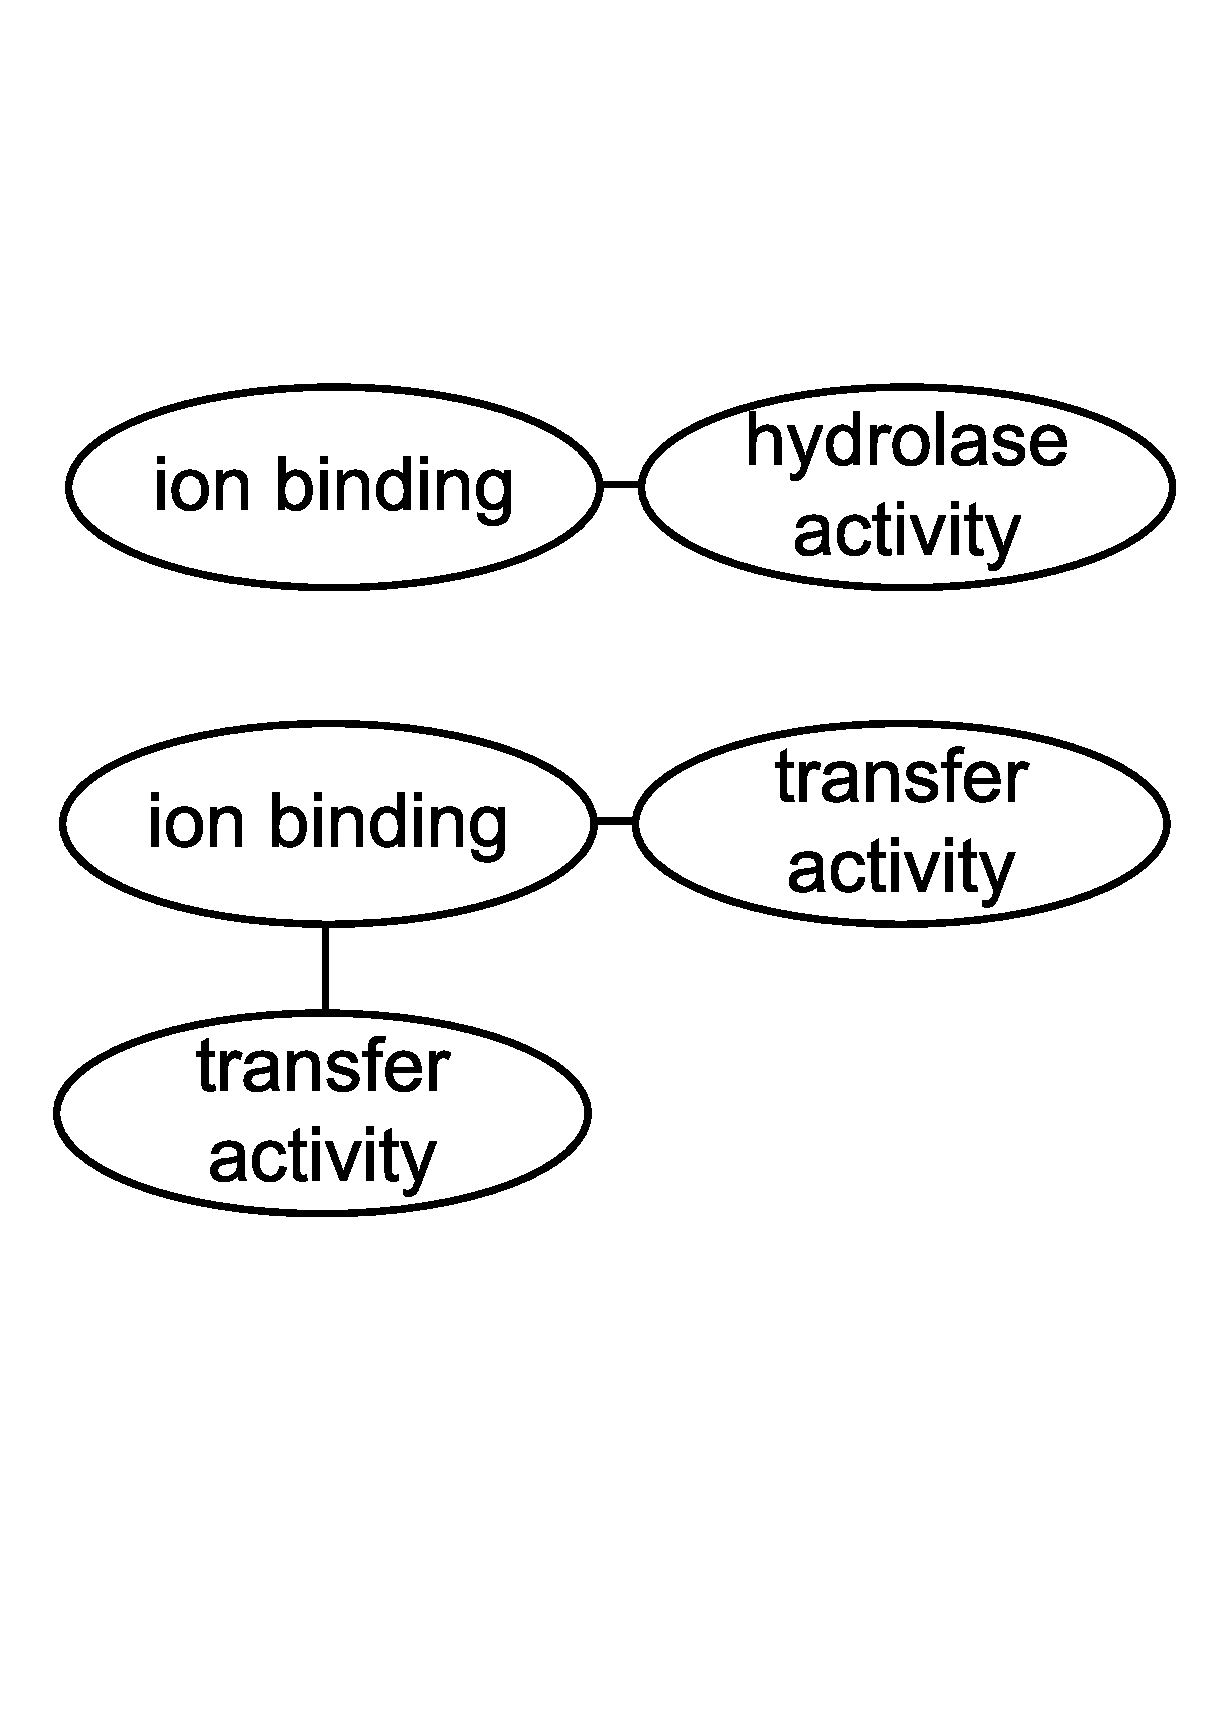
\includegraphics[scale=0.17]{images/yeast1}
%\label{fig:yeast1}
%}
%\subfigure[]  {
%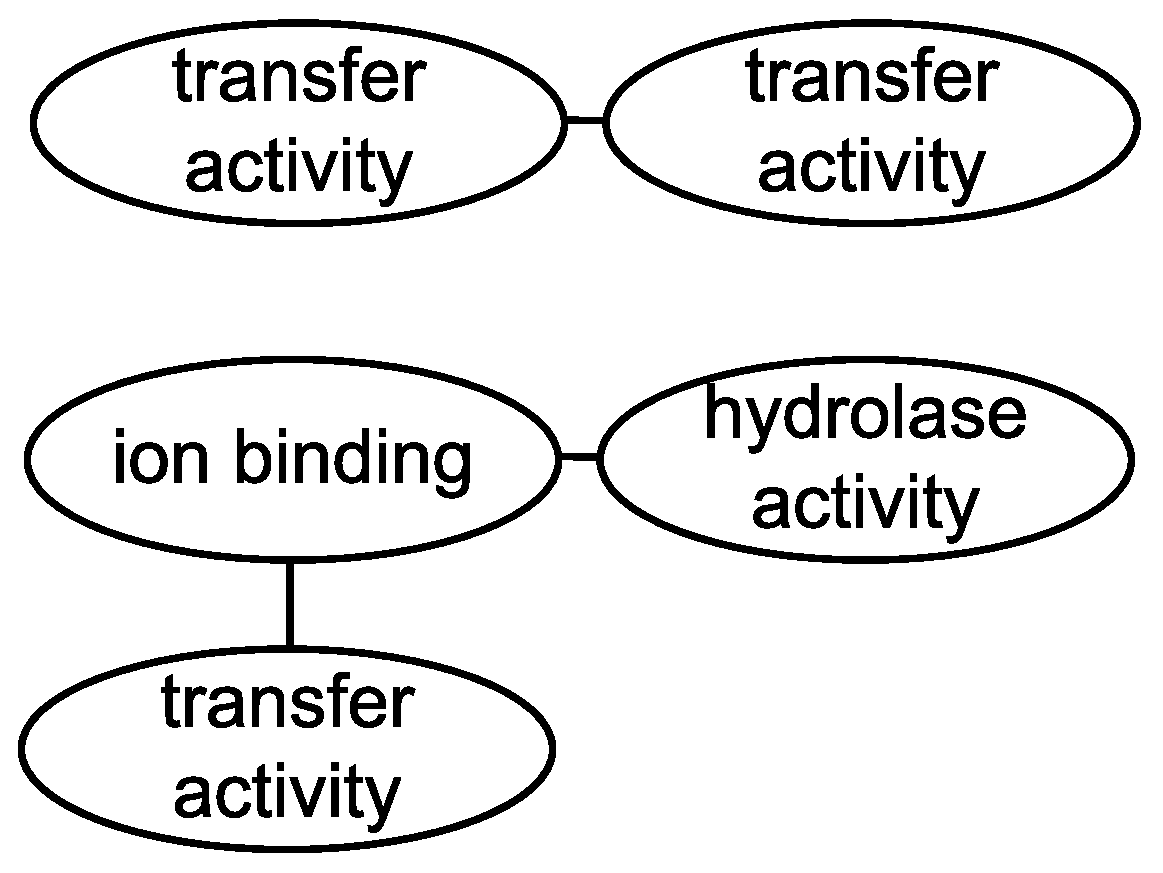
\includegraphics[scale=0.17]{images/yeast2}
%\label{fig:yeast2}
%}
%\subfigure[]  {
%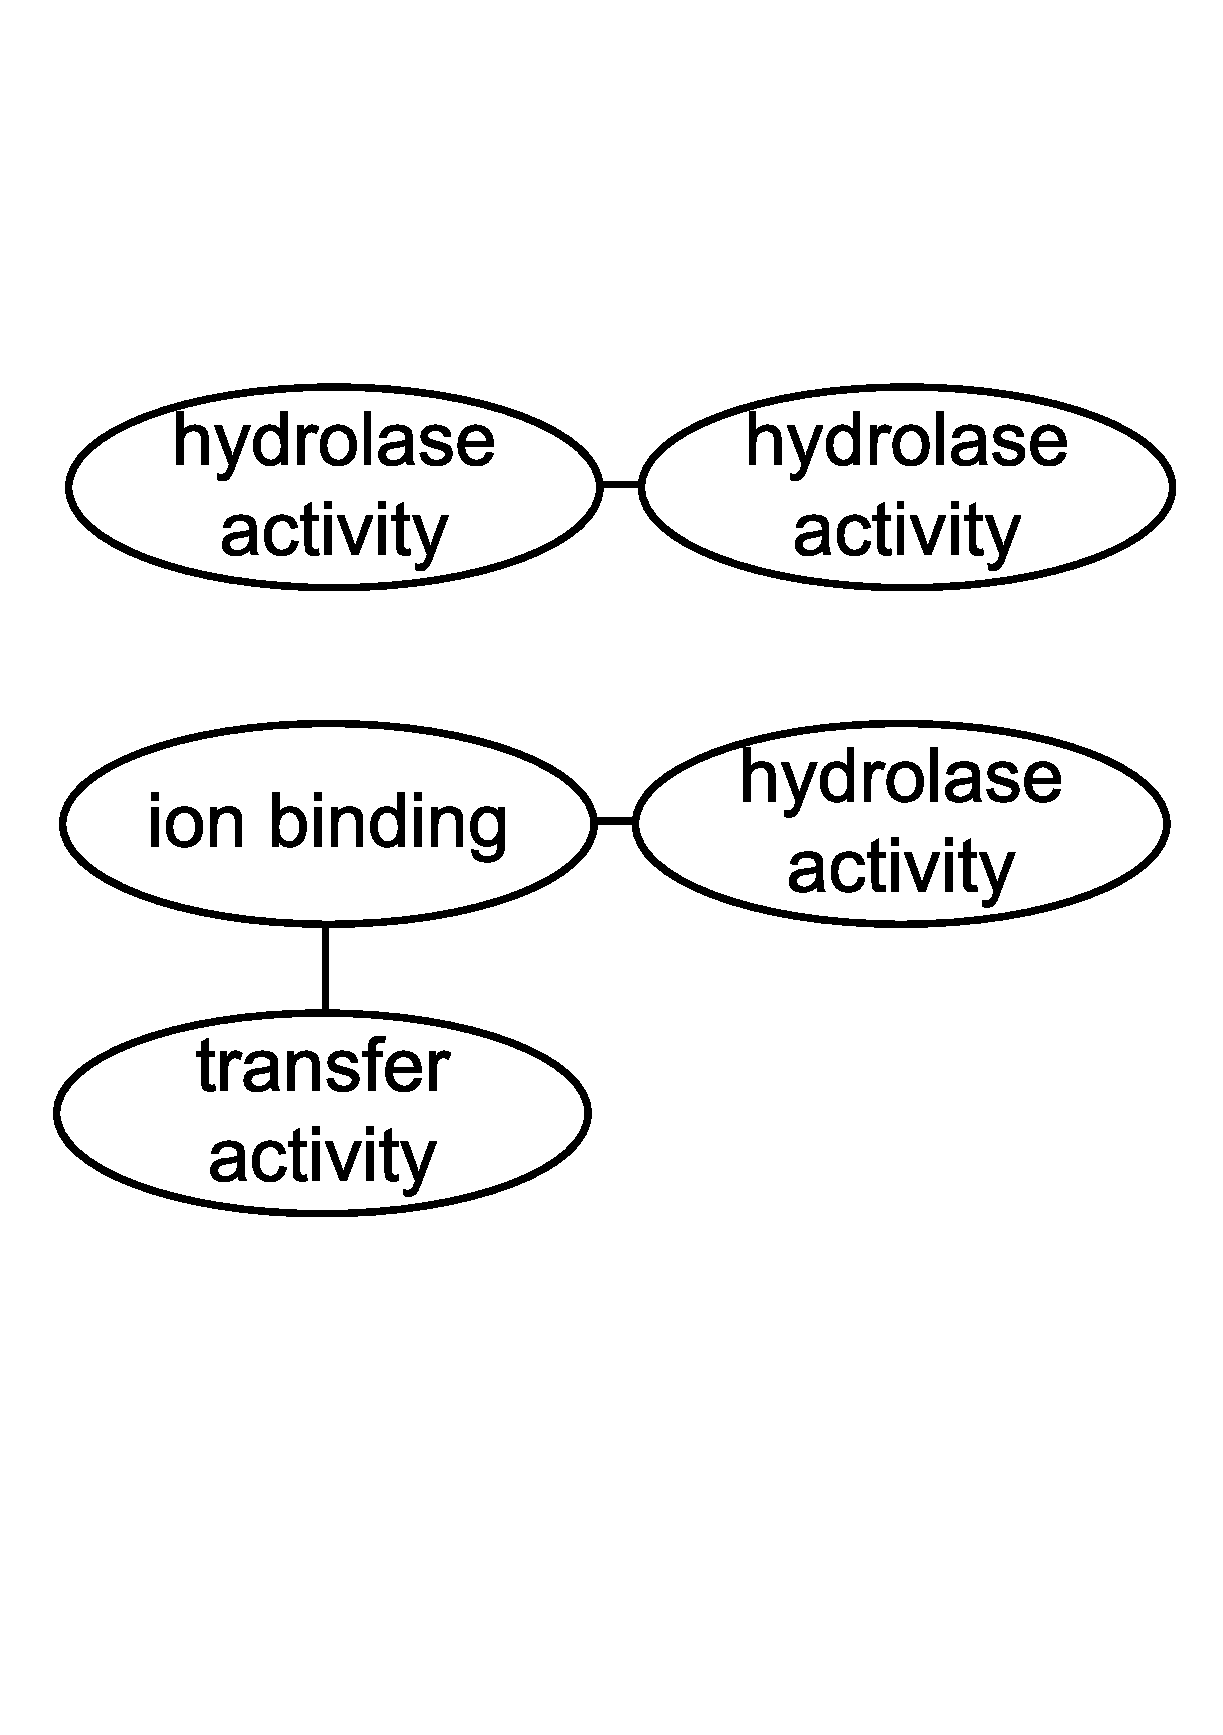
\includegraphics[scale=0.17]{images/yeast3}
%\label{fig:yeast3}
%}
%\vspace{-2mm}
%\caption{\scriptsize Correlated subgraphs discovered in the {\em Yeast} protein dataset. Nodes are annotated with protein functions (node labels).}
%\label{fig:yeast}
%\vspace{-6mm}
%\end{figure}


%\spara{$\bullet$ Difficulties with Proximity Patterns.} Recently, various approximate-frequent-subgraphs mining techniques have been
%proposed, e.g., proximity patterns \cite{KYW10} that relax the rigid structure constraint of frequent subgraphs. In stead, they identify
%a group of node labels that co-occur frequently in the neighborhood. However, such proximity patterns are often unable to capture
%the semantics of our novel correlated subgraphs. As an example, in Figure~\ref{fig:yeast},
%we present three correlated patterns identified from
%the {\em Yeast} (Saccharomyces cerevisiae) protein dataset \cite{}, where protein functions are used as node labels. These
%correlated patterns indicate that {\em transferase} and {\em hydrolase} activities are associated with {\em ion} binding,
%which is due to the fact that {\em transferase} and {\em hydrolase} undergo motions upon ligand ({\em ion}) binding
%to achieve their functions \cite{KAOK08}. However, {\em transferase} and {\em hydrolase} catalyze different chemical
%reactions and express different dynamic responses upon ligand ({\em ion}) binding. It means that {\em hydrolase} and {\em transferase}
%activities are usually not connected with each other directly and they usually connect to {\em ion} binding \cite{KKO09}.
%This is indeed reflected in our discovered correlated patterns, because there is no direct edge between {\em hydrolase} and {\em transferase}.
%On the other hand, the proximity pattern mining algorithm \cite{KYW10} reports
%$\langle${\em hydrolase}, {\em transferase}, {\em ion binding}$\rangle$ as one
%proximity pattern, thus it is unable to capture the fact that {\em hydrolase} and {\em transferase}
%activities are not connected with each other directly.

\spara{Our contributions and roadmap.}
To this end, we design a single-step, best-first exploration algorithm to detect correlated subgraphs,
coupled with efficient top-$k$ pruning and various optimization techniques.
The main contributions of this paper are as follows:
\squishlist
\item
\item
\item
\item We empirically demonstrate effectiveness and efficiency of our methods on real-life graphs,
while also detailing three concrete case studies (Section \ref{sec:experiments}).
\squishend
% }


\section{Preliminaries}
\label{sec:preliminaries}

\subsection{Background}
\label{sec:background}

An attributed graph $G = (V,E,L)$ has a set of nodes $V$, a set of edges
$E \subseteq V \times V$, and a label set $\mathbb{L}$ such that
every node $v \in V$ is associated with a label, i.e., $L(v) \in \mathbb{L}$.
In this work, we focus on bidirectional, node-labeled, and un-weighted
graphs. However, the proposed models and algorithms can also be applied to directed
and edge-labeled graphs.

\spara{Subgraph Isomorphism.} Given an input graph $G=(V,E,L)$, a graph pattern
$Q=(V_Q,E_Q,L_Q)$, a subgraph isomorphism is an {\em injective function} $M: V_Q \rightarrow V$ s. t.
(1) $\forall v\in V_Q, L_Q(v)= L(M(v))$, and (2) $\forall(v_1,v_2) \in E_Q, (M(v_1),M(v_2))\in E$.

Subgraph isomorphism is depicted in Figure~\ref{fig:subgraph_isomorphism}. $M$ is called a subgraph-isomorphic
{\em mapping}. The nodes $\{M(v):v\in V_Q\}$ and the corresponding edges $\{(M(v_1),M(v_2)):(v_1,v_2)\in E_Q\}$
form a subgraph-isomorphic {\em instance} of $Q$ in $G$.
There can be many subgraph-isomorphic mappings and instances of $Q$, e.g., in Figure~\ref{fig:subgraph_isomorphism}
another mapping $M_1$ could be as follows: $M_1(v_1)= u_3$, $M_1(v_2)= u_2$, $M_1(v_3)= u_7$. Clearly, two different
instances of the same pattern may overlap, as in our current scenario: the two instances, defined by mappings $M$
and $M_1$, overlap at nodes $u_2$ and $u_3$,
and also on the edge $(u_2,u_3)$.
%
\begin{figure}[t!]
\centering
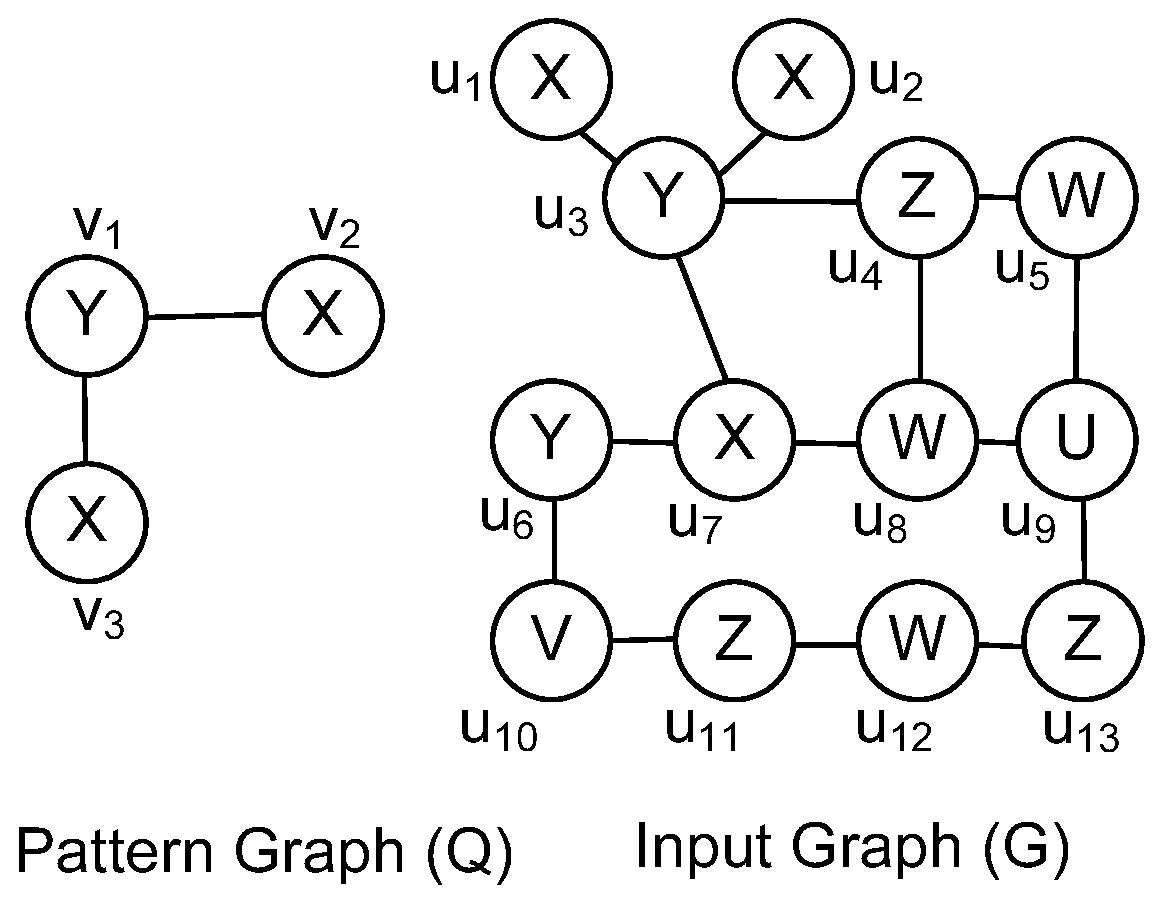
\includegraphics[scale=0.23]{images/subgraph_isomorphism}
\vspace{-2mm}
\caption{\small Subgraph isomorphism: $M(v_1)= u_3$, $M(v_2)= u_1$, $M(v_3)= u_2$. Two other subgraph-
isomorphic mappings could be as follows: $M_1(v_1)=u_3$, $M_1(v_2)=u_1, M_1(V_3)=u_7$; and
$M_2(v_1)=u_3, M_2(v_2)=u_2, M_2(v_3)=u_7$.}
\label{fig:subgraph_isomorphism}
\vspace{-5mm}
\end{figure}

\spara{Support.}
To find frequent subgraphs from a single, large graph, existing literature 
proposed several definitions of subgraph support, denoted as $\sigma$, e.g., maximum independent sets (MIS) \cite{KK04}, 
minimum image-based (MNI) \cite{BN08}, and harmful overlap (HO) \cite{FB07}.
All these metrics are {\em downward-closure}: The support of a supergraph 
$Q_1 \succeq Q$ is higher than that of its subgraph $Q$, i.e., $\sigma(Q_1) > \sigma(Q)$.
However, these metrics differ in the amount of overlap that they allow between subgraph-isomorphic 
instances, and in the complexity of their computation.

In this work, we adopt MNI  \cite{BN08}
due to the following reasons. First, the MNI support
can be efficiently computed; whereas the computation of MIS and HO are \NP-complete \cite{KK04,FB07}.
Second, MNI provides a superset of the results of the two other metrics; thus
the MIS or HO-based results can be identified via an expensive post-processing step,
which prunes out the unqualified subgraphs \cite{EASK14}.
Next, we formally define the MNI support.

\spara{Minimum Image-based (MNI) Support.} Bringmann and Nijssen \cite{BN08} developed the
minimum image-based support. It is based on the number of unique nodes in $G$ that a node of the pattern $Q$
is mapped to. Formally,
%
\begin{align}
\displaystyle \sigma(Q) = \min_{v \in V_Q} |\{M(v) : M \,\text{is a subgraph-isomorphic mapping}\}| &
\end{align}

In Figure~\ref{fig:subgraph_isomorphism}, the MNI support of $Q$ is $1$, which is due to
node $v_1$ having label $Y$, it is mapped to only one node in $G$, i.e., $u_3$ for all three
mappings. The nodes in the set $\{M(v)\}$ for different mappings $M$ are called the {\em images} of $v$.

\spara{Frequent Subgraphs.} Given the input graph $G$, a user-defined minimum-support threshold {\sf Min-Sup}, and
a definition of support $\sigma$, the frequent subgraphs mining problem identifies all subgraphs $Q$ of $G$, such that
$\sigma(Q)\ge$ {\sf Min-Sup}.

\subsection{Problem Formulation}
\label{sec:problem}

Informally speaking, our objective is to identify those pairs of subgraph patterns $\langle Q_1, Q_2\rangle$ such that
they occur closely for a sufficiently large number of times in the input graph $G$. We formalize this notion of
correlation by incorporating the following constraints: (1) The correlation between two subgraph patterns must be
symmetric, and (2) it shall be consistent with respect to the notion of MNI support. 

To be consistent with the MNI support, we group subgraph instances as follows.

\begin{defn}[Instance Grouping]
\label{def:instance_grouping}
Given the input graph $G$, a graph pattern $Q$, and its instances in $G$ denoted as $\mathbb{I}=\{I_1,I_2,\ldots,I_s\}$,
let us define by $v^*$ the node in $Q$ which has the minimum number of images. We denote by
$M(v^*)=\{M_1(v^*),M_2(v^*),\ldots,M_{\sigma(Q)}(v^*)\}$ the images of $v^*$. Notice that
$\sigma(Q)$ is the MNI support of $Q$, $\sigma(Q)\le s$, and $M_j$ is
a mapping of $Q$, for all $1 \le j \le \sigma(Q)$. Next, we form a grouping
of instances, denoted as $\mathbb{I'}=\{I'_1,I'_2,\ldots,I'_{\sigma(Q)}\}$, where
$I'_j= \{I:M_j(v^*) \in I, I \in \mathbb{I}\}$. Intuitively,
$I'_j$ is the group of instances containing the image node $M_j(v^*)$.
\end{defn}
%
\begin{exple}
For input graph $G$ and graph pattern $Q_1$ in Figure~\ref{fig:correlation},
the instances are
given by $\mathbb{I}=\{u_1u_3,u_2u_3,u_7u_3,u_7u_6\}$. However, its MNI support is two, since
node $v_2$ has only two corresponding images: $u_3$ and $u_6$. Thus, we group the instances
according to the presence of $u_3$ and $u_6$ as follows: $\mathbb{I'}=\{u_1u_2u_7u_3,u_7u_6\}$.
\end{exple}

\begin{figure}[t!]
\centering
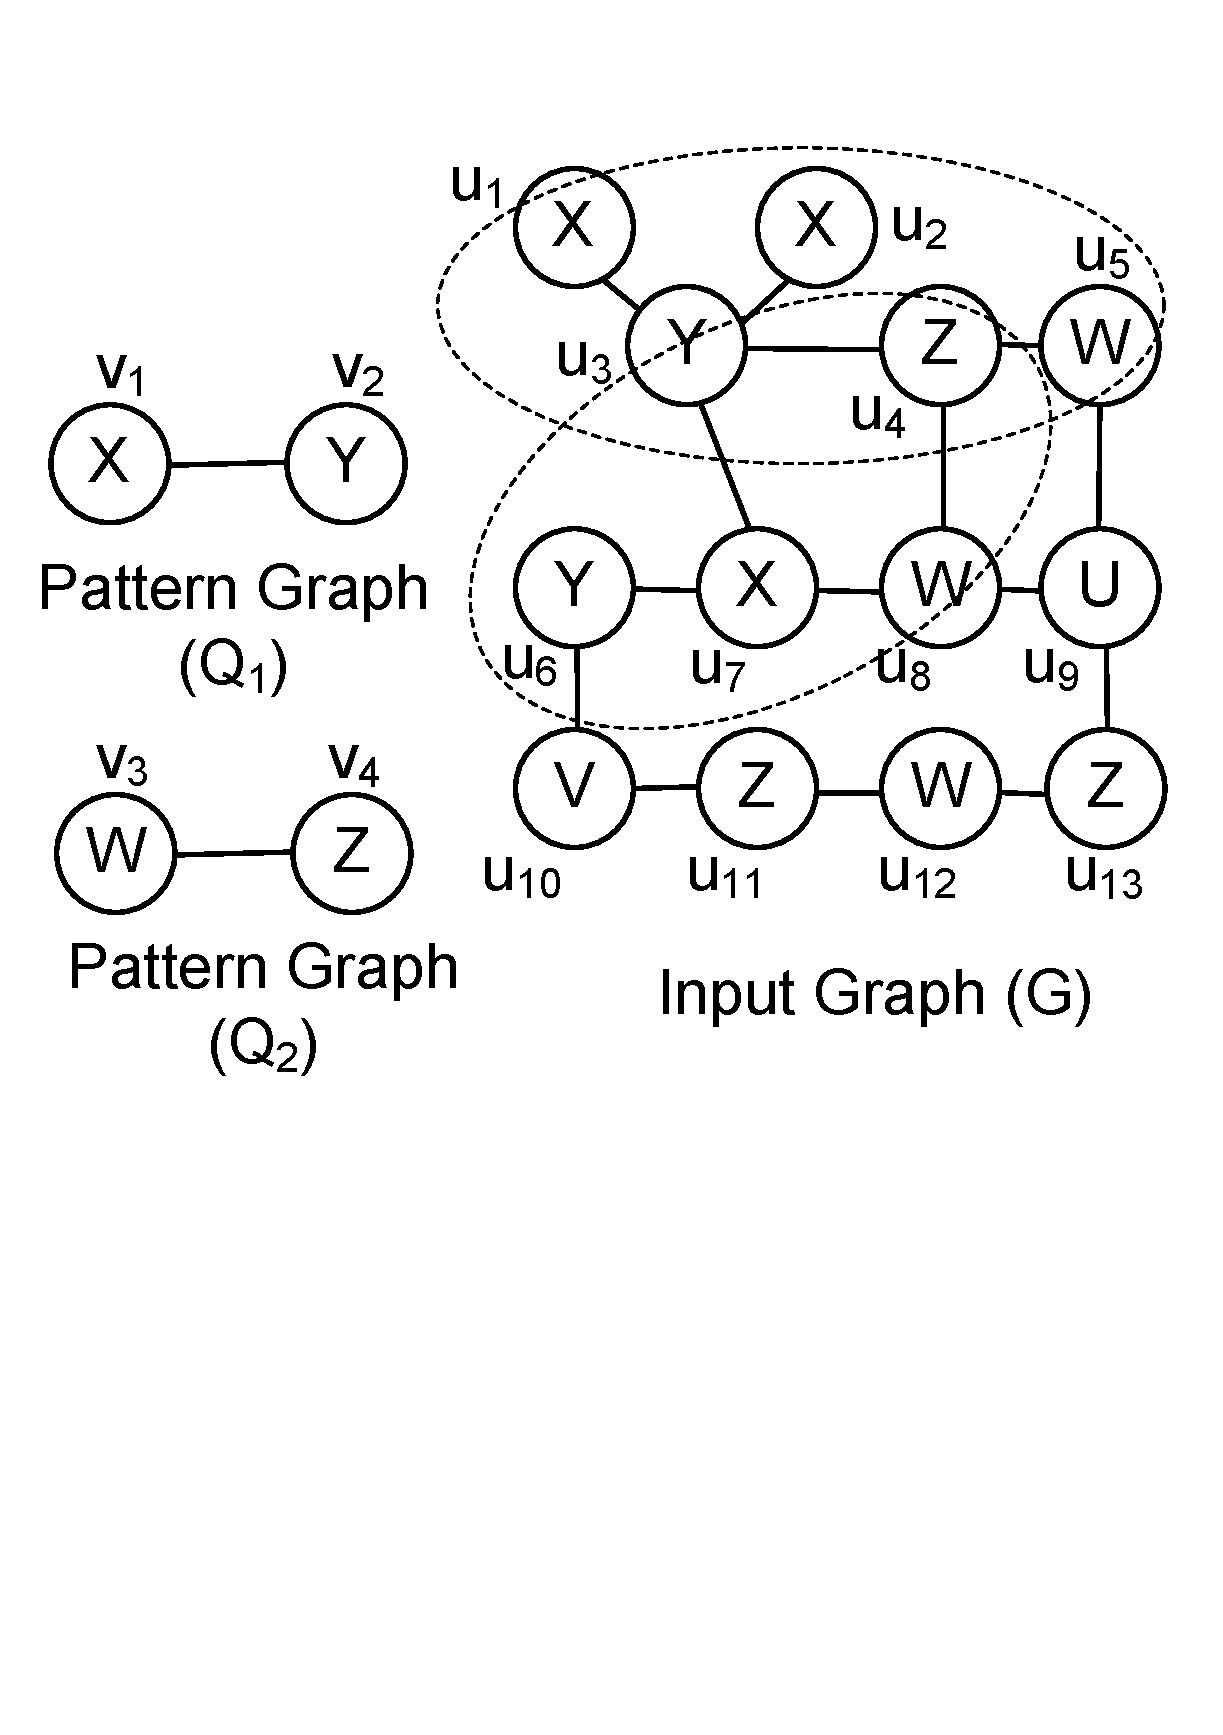
\includegraphics[scale=0.23]{images/correlation}
\vspace{-2mm}
\caption{\small Correlation between subgraphs $Q_1$ and $Q_2$ in $G$}
\label{fig:correlation}
\vspace{-5mm}
\end{figure}

Note that the grouping is not a partition of instances. It is possible for an instance 
to belong to multiple groups, especially when the pattern has multiple nodes with the same label. 
However, for a pattern $Q$, we ensure that the number of instance-groups would be $\sigma(Q)$.

Given two subgraph patterns $Q_1$ and $Q_2$, we compute their instance-groups:
$\mathbb{I'}=\{I'_1,I'_2,\ldots,I'_{\sigma(Q_1)}\}$ and $\mathbb{J'}=\{J'_1,J'_2,\ldots,$ $J'_{\sigma(Q_2)}\}$,
respectively. Without loss of generality, let us assume that $\sigma(Q_1) \le \sigma(Q_2)$. 
Next, we count, out of all $\sigma(Q_1)$  instance-groups of $Q_1$, how many of them are ``close'' to at least
one instance-group of $Q_2$. We report this count as the {\em correlation} between $Q_1$ and $Q_2$ in $G$.
Finally, we define that two instance-groups $I' \in \mathbb{I'}$ and $J' \in \mathbb{J'}$
are close if there exist at least two nodes $u$ in $I'$ and $v$ in $J'$, such that their distance $d(u,v)\le h$,
that is, $u$ and $v$ are no more than $h$-hops away in the input graph $G$.
Clearly, $h$ is a user-defined {\em distance-threshold} parameter that can be varied to support different
amount of closeness between two co-occurrences of $Q_1$ and $Q_2$.

\begin{defn}[Correlation]
\label{def:correlation}
Given two subgraphs $Q_1$ and $Q_2$ in the input graph $G$, their instance-groups
$\mathbb{I'}=\{I'_1,I'_2,\ldots,I'_{\sigma(Q_1)}\}$ and $\mathbb{J'}=\{J'_1,J'_2,\ldots,J'_{\sigma(Q_2)}\}$,
respectively, and a user-defined distance-threshold $h\ge0$,
let us assume that $\sigma(Q_1) \le \sigma(Q_2)$. We define the correlation
$\tau(Q_1,Q_2,h)$ as:
%
\begin{align}
&\tau(Q_1,Q_2,h) \nonumber & \\
&= |\{I' \in \mathbb{I'}:\exists J' \in \mathbb{J'}, \exists u \in I', \exists v \in J', d(u,v)\le h\}|&
\end{align}
\end{defn}

The correlation, for the case $\sigma(Q_2) < \sigma(Q_1)$, can be defined analogously.
We note that the correlation between two subgraphs $Q_1$ and $Q_2$ is {\em symmetric}, that is,
$\tau(Q_1,Q_2,h)$ = $\tau(Q_2,Q_1,h)$.

\begin{exple}
Let us consider two subgraph patterns $Q_1$ and $Q_2$ in the input graph $G$ (Figure~\ref{fig:correlation}),
and the distance-threshold $h=1$. The instance-groups of $Q_1$ are given by: $\mathbb{I'}=\{u_1u_2u_7u_3,u_7u_6\}$,
where the groupings are performed based on the images of node $v_2$ in $Q_1$. Similarly,
the instance-groups of $Q_2$ are given by: $\mathbb{J'}=\{u_5u_4, u_8u_4,u_{11}u_{12}u_{13}\}$,
here the groupings are performed based on the images of node $v_3$ in $Q_2$. We have,
$\sigma(Q_1) =2 < \sigma(Q_2) =3$. Thus, we count, out
of two instance-groups of $Q_1$, how many of them are within $h=1$-hop of at least
one instance-group of $Q_2$. This gives us the correlation $\tau(Q_1,Q_2,h=1)=2$.
\end{exple}

We are now ready to define our problem formally.

\begin{problem}
\label{prob:top-k}
{\bf {\sf Top-$k$} Correlated Subgraphs.}
Given the input graph $G$, a user-defined distance-threshold $h\ge0$, a minimum support threshold $\Sigma$, find the {\em top-$k$} pairs of subgraph patterns $\langle Q_1, Q_2 \rangle$ of $G$, having the
maximum correlations $\tau(Q_1,Q_2,h)$, and for each subgraph pattern $\sigma(Q_1)\ge \Sigma$, $\sigma(Q_2)\ge \Sigma$.
\end{problem}

In the aforementioned problem, if $Q_1$ is a subgraph of $Q_2$, or vice versa, the correlation between them is not interesting.
Thus, in our algorithms, we only identify those pairs which are not related by subgraph and supergraph relationships.


\subsection{Theoretical Characterization}
\label{sec:characteristics}
 
The correlation metric satisfies several interesting properties.

\begin{lma}
\label{lemma:downward}
The correlation metric $\tau(Q_1,Q_2,h)$ is not downward-closure.
\end{lma}

\begin{lma}
\label{lemma:upward}
The correlation metric $\tau(Q_1,Q_2,h)$ is not upward-closure.
\end{lma}

\begin{lma}
\label{lemma:prune}
The following inequality holds: $\tau(Q_1,Q_2,h) \le \min \{\sigma(Q_1),\sigma(Q_2)\}$.
\end{lma}

Lemma~\ref{lemma:prune} directly follows from the definition of correlation (Definition~\ref{def:correlation}), which is computed
from the instance-groups of that subgraph pattern having the smaller support.
\chapter{Exact Algorithm}
\label{sec:exact_algo}

\section{Overview}
\label{subsec:exact_algo_overview}

\begin{observation}
	\label{ob:frequency}
	If two subgraphs have higher support values individually, it is very likely
	that the pair will also have a higher correlation.
\end{observation}

\begin{observation}
	\label{ob:dfs}
	For highly (e.g., top-$k$) correlated subgraphs mining, generally a
	breadth-first or a best-first exploration of the search space is more
	efficient compared to a depth-first traversal of the search space.
\end{observation}

Setting $k$ to infinity would enable us to mine all pairs of correlated subgraph
patterns. However, on the contrary, it is hard to control the value of {\sf
Min-sup} to get the result of a particular $k$ of {\sf Top-$k$} correlated
subgraphs. That is to say, the {\sf Min-Sup} problem can be transfered from {\sf
Top-$k$} problem. As a result, we concentrate on {\sf Top-$k$} problem in the
following sections.

% \setlength{\parskip}{0.3em}
\spara{\raggedleft \textbf{Pattern Search Tree.}} All operations including
correlation computation and subgraph pattern extension are performed on patterns
following an order on a \textit{pattern search tree}. We denote this tree as
$T$. Each node $Q\in T$ represents a subgraph pattern. We denote the set of
current \textit{leaf} nodes in $T$ as $Leaf(T)$. Each element $Q_l\in Leaf(T)$
is a pattern that has not yet been $operated$ for correlation computation. A
node $Q_l\in Leaf(T)$, once operated, is inserted into the $operated$ set.
% \setlength{\parskip}{0em}

% \subsection{Order of Subgraph Generation and Correlation Calculation}

\par The correlated subgraph mining algorithm is an iterative procedure,
essentially consisting of the following steps: \par 1) select a node $Q_i$ from
$Leaf(T)$, i.e. $Q_i\in Leaf(T)$, and pop out $Q_i$ from $Leaf(T)$, i.e.
$Leaf(T)=Leaf(T)\setminus Q_i$. \par 2) calculate $\tau(Q_i,Q_j,h)$, for all
$Q_j\in operated$ \par 3) try to extend $Q_i$ to $Ex(Q_i)$, where $Ex(Q_i)$ is
the set of all the possible subgraphs extended from $Q_i$. \par 4) Check the
frequency of $Q_i',Q_i'\in Ex(Q_i)$ based on MNI support, $\sigma(Q')$, if
$\sigma(Q_i')\ge$ {\sf Min-Sup}. we put $Q_i'$ into $Leaf(T)$.
\begin{thrm}
	The order of subgraph generation and correlation calculation will not miss
	any correlated pairs between any of two frequent subgraphs.
\end{thrm}
% After step 4, we give $Q_i'$ an index of frequent subgraph discovery order,
% denoted as $index(Q_i')=a$, which means $Q_i'$ is the $a$-th subgraph in $T$.
% After the loop, we give $Q_i$ an index of correlation calculation order,
% denoted as $corIndex(Q_i)=b$, which means $Q_i$ is the $b$-th subgraph in $T$
% which and we put $Q_i$ into $Cor(T)$, i.e. $Cor(T)=Cor(T)\cap Q_i$.

\subsection{Best-first Exploration}
\label{subsubsec:exact_algo_bestfs}
Observation \ref{ob:frequency} suggests that faster convergence of the algorithm
could be expected if a subgraph pattern having a higher support is
\textit{operated} preceding every other pattern in $Leaf(T)$. As a result, we
use a naive rule to determine the priority of the leaf nodes in $Leaf(T)$: $Q_1$
has a higher priority than $Q_2$ \forall $Q_1, Q_2 \in Leaf(T)$ if and only if:
\begin{align*}\sigma(Q_1)>\sigma(Q_2)\end{align*}
Utilizing the estimating rule above, if the current leaf node $Q_k$ in the search tree has a highest support among all the other elements in the set of the leaf nodes, i.e. $\sigma(Q_k)=\max\{\sigma(Q_i)|Q_i\in Leaf(T)\}$. Then, $Q_k$ has the priorty to be calculated and extended.


\subsection{Termination Criteria}
\label{subsubsec:exact_algo_ceasing}
Obviously, our purpose is to find $k$ pairs of correlated subgraphs and guarantee that the other pair of subgraphs could not have a higher correlation $\tau$. Retrospect the properties mentioned in Section \ref{sec:overview}, assume $Q$ is a frequent subgraph of the data graph, $Q_k$ is an arbitary frequent subgraph of the data graph. We denote $Sup(Q)$ as the set of all the possible supergraphs of $Q$ and $Q'\in Sup(Q)$. Then, the following condition always holds:
\begin{align*} \tau(Q',Q_k,h)\le \sigma(Q') \end{align*}
\begin{align*} \sigma(Q')\le \sigma(Q) \end{align*}
It is easy to get following upperbound of $\tau(Q',Q_k,h)$ by combining the two conditions above:
\begin{align*} \tau(Q',Q_k,h) \le \sigma(Q) \end{align*}
Consider this upperbound, if $\sigma(Q)$ does not reach the minimum number of
being a candidate of {\sf Top-$k$} set, i.e. $\sigma(Q)<\tau(Q_i,Q_j,h)$ for all
the $i, j$ in the current {\sf Top-$k$} set, then all the correlations
containing $Q$, $\tau(Q,Q_k,h)$, as well as all the correlations containing
$Q'$, $\tau(Q',Q_k,h)$, are impossible to be the elements in {\sf Top-$k$} set.
\par On the other hand, we have to consider another possible circumstance, where
there are no $k$ correlated pairs in this graph at all. In that case, the number
of elements in {\sf Top-$k$} set has not reached $k$ but all the support value
of the leaf nodes are already below the minimum support. As a consequence, this
condition is also a signal telling us to stop the search. \par Formally, we fix
the condition of not adding $Q$ to $Leaf(T)$, which is, suppose $|Topk|$ is the
number of elements in {\sf Top-$k$} set, $min\_sup$ is the minimum support of
the correlation, we stop our search if either both of the following conditions
holds.
\begin{align*} \sigma(Q)\le min\{t|t\in Top\_k\}\end{align*}
\begin{align*} |Top\_k|=k \end{align*}
or following condition holds.
\begin{align*} \sigma(Q)\le min\_sup\end{align*}
In this case, all the $Q,Q\in Leaf(T)$ is possible to have the correlation we want. Obviously, on the other hand, if $Leaf(T)=\emptyset$, we report all the {\sf Top-$k$} correlated subgraphs and cease our search.
\begin{figure}[t!]
	\centering
	\includegraphics[scale=0.32]{images/ceasing_condition}
	\vspace{-2mm}
	\caption{\scriptsize For 3 subgraphs $Q_1,Q_2,Q_3$, with $\sigma(Q_1)=5$, $\sigma(Q_2)=2$, $\sigma(Q_3)=3$. The current {\sf Top-$k$} set is $\{4,5,6\}$, the input parameters are $k=3$, {\sf Min-sup}$=3$}.
	\label{fig:ceasing_condition}
	\vspace{-6mm}
\end{figure}
\begin{exple}
	In Figure \ref{fig:ceasing_condition}, the minimum element in {\sf Top-$k$} set is $4$, $Q_1$ is the only leaf node at the beginning, i.e. $Leaf(T)=\{Q_1\}$ and $\sigma(Q_1)>4$ so that $Q_1$ can be extended to $Q_2,Q_3$. After extension, $Q_1\notin Leaf(T)$ and $Leaf(T)=\{Q_2,Q_3\}$. $Q_2<$ {\sf Min-sup}, and $Q_3=$ {\sf Min-sup} but $Q_3<4$, and there are already $3$ elements in {\sf Top-$k$} set, i.e. $|Top\_k|=3$. Thus, all the correlation of $Q_2,Q_3$ would not satisfies the condition we want and we cease the search.
\end{exple}



\section{Replica-based Graph Instance Storage}
\label{subsec:replica-storage}

\subsection{Replica Graph Data Structure}
\label{subsubsec:replica-ds}
Considering the large amount of overlaps of the instances in dense graph, we use a novel structure to store a subgraph pattern, which not only get rid of the expensive cost of tackling dense graph, but also be the robust foundation of carrying out an efficient correlation calculation based on instance grouping.
\par Our search tree storage unit is extremely direct and naive. Instead of considering the instances of a pattern, we just create a reproduce of the occurrences of the vertices and the edges of the pattern, called {\bf replica}. We record all the vertex identifications and the edge connections in the replica, we do not record the edge labels.
\begin{figure}[h!]
	\vspace{-2mm}
	\centering
	\subfigure[{\scriptsize Subgraph Pattern $Q$}] {
		\includegraphics[scale=0.33]{images/replica1}
		\label{fig:replica1}
	}
	\subfigure[{\scriptsize Occurrence of $Q$}]  {
		\includegraphics[scale=0.30]{images/replica2}
		\label{fig:replica2}
	}
	\subfigure[{\scriptsize Replica of $Q$}]  {
		\includegraphics[scale=0.25]{images/replica3}
		\label{fig:replica3}
	}
	\vspace{-2mm}
	\caption{\scriptsize All the edge in Figure \ref{fig:replica2} from $A$ to $B$, $B$ to $C$ has the edge label $a,b$ respectively. Figure \ref{fig:replica3} is replicated from Figure \ref{fig:replica2} without edge labels.}
	\label{fig:replica}
	\vspace{-6mm}
\end{figure}
% \newline
\newline
% As {\sf Found($Q$)} occurs, we store the replica of $Q$ as a unit of the search tree. 
After $Q$ has been $operated$, we remove $replica(Q)$ from memory.

\spara{$\bullet$ Replica Unit.} The illustration of replica is as Figure \ref{fig:replica}. The details of replica is as follows.\\1) For each $Q\in T$, there is a corresponding replica $R(Q)$.\\2) For each $u_i\in Q$, there is a hash-map, $R_i(Q)$, recording the vertex identifications, and $R(Q)=(R_1(Q), R_2(Q), ..., R_{|V_Q|}(Q))$.\\3) For each element $v\in R_i(Q)$, there is a record of all the other vertices which $v$ is connected to in the occurrences of $Q$.

\subsection{Generation of a Replica Graph}
\label{subsubsec:replica-gen}
Algorithms 1 and 2 together describe the complete procedure to construct the replica graph for a subgraph pattern. Replica construction for any pattern $R$ requires knowledge of the replica graph of the pattern $Q$ that is extended to generate it. Henceforth, we refer to such a pattern $R$ as a $child\ pattern$ of $Q$ and $Q$ as the $parent\ pattern$ of $R$. Since the search procedure processes a pattern only after its parent, the replica graph of the $parent\ pattern$ can be used for constructing the replica graph of the $child\ pattern$.
% \begin{algorithm}
% 	\DontPrintSemicolon
% 	\dontprintsemicolon
% 	\KwIn{Training sentences $S_{i}$}
% 	\KwOut{Sentence instances with cost-vectors for training $S_{i,c_i}$}
% 	\SetKwBlock{Begin}{function}{end function}
% 	\Begin($\text{generateCosts} {(} EV_{i,v,r} {)}$)
% 		{
% 	$S_{i,c_{i}} = \left[ \right]$\;
% 		\ForAll{$s \in S, v \in EV $}
% 		{
% 			$c_{i} = \left\lbrace \right\rbrace$\;
% 			set $region \; r = EV_{i,r}$\;
% 			\For{$p \leftarrow 1, properties$}
% 			{
% 				$c_{i,p} \coloneqq cost \left( kb_{r,p},v_{i,r} \right)$\;
% 				\uIf{$c_{p} > Cost_t$}
% 				{
% 					$c_{p} \coloneqq \infty$
% 				}
% 				\Else
% 				{
% 					continue
% 				}
% 			}
% 			\uIf{$\min \left( c \right)  > APE_t$}
% 			{
% 				$c_{i,no\_property} \coloneqq 0$
% 			}
% 			\Else
% 			{
% 				$c_{i,no\_property} \coloneqq \infty$
% 			}
% 			$\text{push} \left( S_{i,c_{i}}, \left( s,c_{i} \right) \right)$
% 		}\label{endfor}
% 		\Return{$S_{i,c_{i}}$}
% 	}
% 	\caption{Cost-Vector Algorithm}\label{costalgorithm}
% \end{algorithm}

\begin{algorithm}
	% \begin{algorithmic}[1] 
	% \REQUIRE input graph: $G$, parent pattern: $Q$, replica of $Q$: $replica(Q)$, extending index: $u$, tuple of extension vertex label and extension edge label: $candidate\ edge$, child pattern: $R$
	% \ENSURE all mappings of child pattern $R$ in $G$ (that is, the replica of $R$: $replica(R)$ in $G$)
	\dontprintsemicolon
	% \KwIn{Graph $G$, parent: $Q$, $replica(Q)$, extending index: $u\in V(Q)$, extension: $candidate\ edge$, child: $R$}
	\nonl \textbf{Input:} Graph $G$, parent $Q$, $replica(Q)$, child $R$, extending index: $u\in V(Q)$, extension: $candidate\ edge (u,v) \in E(R)$\;
	% \KwOut{$replica(R)$}
	\nonl \textbf{Output:} $replica(R)$ \;
	% \SetKwBlock{Begin}{function}{end function}
	% \Begin($\text{generateCosts} {(} EV_{i,v,r} {)}$)
	% {		
	$DFS\ List\leftarrow$ get rooted \textsc{DFS} of $Q$ with $u$ as $root$ \;
	$instance \coloneq \emptyset$\;
	\ForEach{ $u' \in Mappings(u,\ replica(Q))$}
	{
		$instance\leftarrow \{(u,u')\}$ \;
		\ForEach{\textup{edge} $e(u',v')\in E(G)$ \textup{that maps to} $candidate\ edge (u,v)$}
		{
			$instance\leftarrow instance \cup \{(v,v')\}$\;
			$\mathbb{I}\leftarrow$ \textsc{FindAllInstances($R$, $instance$, $\mathbb{I}$, $DFS\ List$, ...)}\;
			\textsc{UpdateReplica($replica(R)$, $\mathbb{I}$, ...)}\;
			$instance\leftarrow instance \setminus \{(v,v')\}$\;
			% Append all edges in $\mathbb{I}$ to $replica(R)$ and update the mappings list for every vertex\;
		}
		$instance\leftarrow instance \setminus \{(u,u')\}$\;
	}
	\Return{$replica(R)$}
	% }
	\caption{\textsc{GetReplica}}\label{algo:search}
	% \end{algorithmic}
\end{algorithm}

Algorithm 1 essentially describes a procedure to find every mapping (also referred to as $instance$) of the $child\ pattern$ in the input graph using the mappings of the $parent\ pattern$ and thus obtain its $replica$ graph. The algorithm begins with a depth-first search ({\sf DFS}) procedure (line 1) executed on the $parent\ pattern\ Q$, selecting the vertex from which the $candidate\ edge$ is extended as the $root$. We call this vertex the $extending\ vertex$ in $Q$. The edges encountered in the depth-first traversal are recorded in an ordered list called the $DFS\ List$, which helps guide the instance enumeration procedure performed subsequently. The algorithm iterates over all mappings of the $extending\ index$ in the $replica$ of the $parent\ pattern$ (line 2) and attempts to enumerate all (if any) instances of the $child\ pattern$ in the data graph one-by-one. More specifically, for every vertex $m$ of $replica(Q)$ that maps to the $extending\ vertex\ u$, the algorithm iterates over its adjacent edges in the input graph that map to the $candidate\ edge$ (line 3) and invokes the {\sf find\ all\ instances} method (Algorithm 2) to enumerate every $instance$ of $child\ pattern\ R$ from $replica(Q)$ that contains this adjacent edge. Algorithm 2, thus invoked, recursively enumerates all instances of $R$ in a depth-first manner following the $DFS\ List$ of $Q$ (computed earlier). In the general case (lines 4-10), the algorithm selects an appropriate graph edge as the mapping of an edge in the $child\ pattern\ R$ (line 5) and recursively invokes the method to find a mapping of the next edge in the $DFS\ List$ that is consistent with the edge mappings selected so far (line 7). Once all edges in the $DFS\ List$ have been mapped to graph edges, the base case (lines 1-3) gets executed where the instance of $R$ thus enumerated is simply returned. Thus, the set of all instances found is returned at the end of Algorithm 2 (line 10) and recorded by Algorithm 1 to update the $replica$ graph (line 6, Algorithm 1). In the update step, the algorithm simply appends all edges of every instance in $\mathbb{I}$ to the existing set of edges of $replica(R)$, and also updates the $mappings\ set$ for every vertex of pattern $R$ to include the vertices of the newly-discovered instances in $\mathbb{I}$.
% The {\sf find all instances()} function used in Algorithm ? is defined below. It enumerates all instances in a depth-first manner starting from the $extending\ index$ as the $root$ by following the {\sf DFS} edge-ordering stored in $DFS\ List$.
\begin{algorithm}
	\dontprintsemicolon
	\caption{\textsc{FindAllInstances} \textsc{(Exact)}}\label{algo:complete-instances}
	\nonl \textbf{Input:} Graph $G$, parent $Q$, $replica(Q)$, child $R$, $DFS$ $List$, partial isomorphism of $R$: $instance$, $\mathbb{I}$\;
	% parent edge: $(u, v)\in E(G)$ mapped to $(u',v')\in E(R)$,
	% \KwOut{$replica(R)$}
	\nonl \textbf{Output:} $\mathbb{I}: $ set of all instances of $R$ in $G$ consistent with input partial isomorphism $instance$\;
	%such that $\forall I \in \mathbb{I} $  $ (u',u),(v',v) \in I$)\;
	% \REQUIRE input graph: $G$, parent pattern: $Q$, replica of $Q$: $replica(Q)$, parent edge: $(u, v)$, $DFS\ List$ of $Q$ rooted at $extending\ index$, child pattern: $R$
	% \ENSURE all mappings of pattern $R$ in $G$ that include $(u, v)$
	\uIf{$|instance|=|V(R)|$}
	{
		\Return{$instance$}
	}
	\Else
	{
		$e(p,c) \coloneq$ \textsc{NextQueryEdge($DFS\ List, ...$)}\;
		$P_{c} \coloneq$ \textsc{FilterCandidates($instance, c, ...$)}\;
		\ForEach{$w \in P_{c}$ \textup{such that w is not yet matched}}
		{
			$instance \leftarrow instance \cup \{(c,w)\}$\;
			$\mathbb{I} \leftarrow \mathbb{I}\ \cup$ \textsc{FindAllInstances($R,instance,$ ...)}\;
			$instance \leftarrow instance \setminus \{(c,w)\}$\;
		}
		\Return{$\mathbb{I}$}\;
	}
	% \IF{all $edges$ in $DFS\ List$ have been mapped}
	% \STATE \textbf{return} $instance$ set
	% \ENDIF
	% \FORALL{adjacent edges $e$ of $v$ in $replica(Q)$}
	% \IF{$e$ maps to the corresponding $child\ edge$ in $DFS\ List$ \textbf{and} \textbf{not} already in $instance$}
	% \STATE $instance\leftarrow instance\cup e$
	% \STATE $\mathbb{I}\leftarrow \mathbb{I}\ \cup\ ${\sf find\ all\ instances($R$, $e$, $instance$, $DFS\ List$)}
	% \STATE $instance\leftarrow instance \setminus e$
	% \ENDIF
	% \ENDFOR
	% \STATE \textbf{return} $\mathbb{I}$
\end{algorithm}

This replica storage strategy not only builds a foundation for the sequential efficient correlation calculation, but also benefits the MNI support counting in the single large graph since we can directly get $\sigma(R)$ when we record the replica of $R$ just by counting all the sizes of the images $M(v)$, where $v\in R$.


\subsection{Indexing to Facilitate Replica Deletion}
\label{subsubsec:replica-indexing}

\section{Subgraph Extension}
\label{subsec:subgraph-ext}
\subsection{Extension Rule}
We subscript the node patterns in a subgraph patterns to identify their order of discovery.
\begin{defn}[Vertices Subscripting]
	Let $Q$ be a frequent subgraph in $T$, apart from vertex identification $v_i$, we use another metric to subscript the vertices in $Q$ by the order we discover the pattern $Q$, denoted as $S_Q=(s_0,s_1,...,s_n)$, where $n=|V_Q|$. And for $s_i$ and $s_j$, if $i<j$, then the vertex $v_i$ is discovered earlier than the vertex $v_j$.
\end{defn}
Taking advantage of subscripting, it is easy to get the right-most path of a subgraph. Then, we only grow the new vertices in right-most path. Corresponding to the best-first-search strategy, the node with highest MNI support will be chosen, suppose $Q$. Then, for all the vertices in its right-most path of the replica of $Q$, we try one edge extension from them respectively, see Algorithm \ref{algo:extension}.

\begin{algorithm}
	\dontprintsemicolon
	% \begin{algorithmic}[1]
	\nonl \textbf{Input:} Graph $G$, parent $Q$, $replica(Q)$ \;
	\nonl \textbf{Output:} $Ex(Q)$: set of candidate edge extensions for $Q$\;
	% \REQUIRE data graph $G$, subgraph pattern $Q$, replica of $Q$, {\sf Min-sup}
	% \ENSURE frequent pattern set extended from $Q$, $Ex(Q)$
	$Ex(Q)\coloneq \emptyset$ \;
	$rmpath \leftarrow$ right-most path of $Q$ from $DFS\ Code(Q)$\;
	\ForEach{$v\in rmpath$}
	{
		\ForEach{$v'\in Mappings(v,replica(Q))$}
		{
			$E\leftarrow$ set of all edges $(v',w')\in E(G)$ extending $Q$\;
			$Ex(Q)\leftarrow Ex(Q)\cup E$
		}
	}
	\Return{$Ex(Q)$} 
	% \STATE $Ex(Q)\leftarrow\emptyset$
		% \STATE $Rmpath\leftarrow$ right-most path of $Q$
		% \FORALL{$s$ in $Rmpath$}
		% \STATE $Ex(Q)\leftarrow Ex(Q)\cup$ possible extensions
		% \ENDFOR
		% \FORALL{$ex$ in $Ex(Q)$}
		% \IF{$\sigma(ex)<$ {\sf Min-sup}}
		% \STATE $Ex(Q)\leftarrow Ex(Q)\setminus ex$
		% \ENDIF
		% \ENDFOR
		% \RETURN $Ex(Q)$
	% \end{algorithmic}
	\caption{\textsc{SubgraphEdgeExtensions}}\label{algo:extension}
\end{algorithm}

\subsection{Duplicated Subgraph Prunning}
To avoid the duplicated subgraph judgement, we take the advantage of the DFS code, and the minimum DFS code in gSpan\cite{YH02}, whenever a subgraph is founded, we get its DFS code, denoted as $C(Q)$ and remodel this subgraph by using this code. Then, we build the minimum DFS code of this subgraph $Q$. This minimum DFS code, denoted as $Z(Q)$ is the canonical label of this subgraph in our definition.

\par We use a dictionary $\mathbb{D}$ to store all the minimum DFS code we have discovered so far. When a subgraph $Q$ is discovered and its graph code $C(Q)$ has been transformed to minimum DFS code $Z(Q)$, we search $Z(Q)$ in the dictionary. If $Z(Q)\in \mathbb{D}$, then $Q$ must have been discovered before, so we prune $Q$.


\section{Correlation Computation}
\label{subsec:corrcomp}

\subsection{Global Index}
\label{subsec:global-index}

We use a global index to record all the distance information. Each vertex of the data graph stores two catogories of distance information.

\squishlist
\item{\bf Proximity Vertices.} For each $u\in G$, we store the information of proximity vertices of $u$, denoted as $CorV(u)$, for each vertex $u\in CorV(u)$, there exists $d(u,v)\le h$.
\squishend
\squishlist
\item{\bf Proximity Patterns.} For each $u\in G$, we store the information of proximity patterns of $u$, denoted as $CorP(u)$, for each pattern $Q\in CorP(u)$, suppose the instance-groups of $Q$ is $\mathbb{I'}=\{I'_1,I'_2,\ldots,I'_{\sigma(Q)}\}$, there exists $I'\in \mathbb{I'}$, $\exists v\in I'$, $d(u,v)\le h$.
\squishend
With the global index acquired before the search, there is no need to consider anything about the distance (hop-constraints) in the search steps. The detail of the maintenance of these two indices is specified in Section \ref{subsec:calculating}.

\subsection{Calculating Correlation}\label{subsec:calculating}
\begin{defn}[Positive Instance Group]
	Given two subgraphs $Q_1$ and $Q_2$ in the input graph $G$, their instance-groups
	$\mathbb{I'}=\{I'_1,I'_2,\ldots,I'_{\sigma(Q_1)}\}$ and $\mathbb{J'}=\{J'_1,J'_2,\ldots,J'_{\sigma(Q_2)}\}$,
	respectively, and a user-defined distance-threshold $h$, assume that $\sigma(Q_1) \le \sigma(Q_2)$.
	Then, we say an instance group of $Q_1$, $I'_i\in \mathbb{I'}$ is a {\bf positive instance group} of $Q_2$ if following condition is satisfied.
	%
	\begin{align}
		\exists J' \in \mathbb{J}, \exists u \in I', \exists v \in J', d(u,v)\le h
	\end{align}
	Then, we denote $P(I'_i,Q_2,h)=1$, otherwise $P(I'_i,Q_2,h)=0$.
\end{defn}
\begin{thrm}
	Let $Q_1,Q_2$ be two subgrpah patterns, and an instance group of $Q_1$, $I'$. Then,	if $Q_2\in \cap CorP(v),v\in I'$, $P(I'_i,Q_2,h)=1$.
	otherwise, $P(I'_i,Q_2,h)=0$.
\end{thrm}
The process of correlation calculation could be considered as a {\bf collection}. Suppose we are calculating the correlation of $Q_1$, i.e. $\tau(Q_1,Q_k,h)$, for all $Q_k\in Cor(T)$. Taking advantage of the global index in Section \ref{subsec:global-index}, by traversing all the vertices in a group can we know the correlation $\tau()$ of all the $v$. We collect these sets one-by-one and finally we could know all the correlation of $Q_1$, i.e. $\tau(Q_1,Q_k,h)$, for all $Q_k\in Cor(T)$.

\subsection{Replica Structure Transformation}
It is more convenient to implement an efficient collection in a hierarchical structure, like tree. As a result, to initialize a collection, we first transform the search space of the collection to a particular tree.
\par Prior to the detailed operations, we first define the group center and the collection tree of a pattern.
\begin{defn}[Group Center and Center Subscript]
	Given a subgraph $Q$, and the instance-groups of $Q$, $\mathbb{I'}=\{I'_1,I'_2,\ldots,I'_{\sigma(Q)}\}$, a group center $u$ of $I'_i$ is the vertex having the minimum MNI support among all $v\in I'_i$, denoted as $u=center(I_i)$, a center subscript is the vertex subscript has the MNI support of the images, denoted as $centerSubscript(Q)$. i.e. $centerSubscript(Q)=i$, where $M(s_i)=\sigma(Q)$.
\end{defn}
\begin{defn}[Collection Tree]
	Given a subgraph $Q$, a collection tree of $Q$, $CT(Q)$ is tree transfromed from the tree structure replica, and rooted at $centerSubscript(Q)$.
\end{defn}
% First of all, if a subgraph contains any backward edges, we remove all its backward edges in its replica prior to the calculation. This is because 1) removing backward edges would not affect the result of correlation calculation. 2) removing backward edges could derive a tree structure subgraph, which is more convenient to carry out the collection.
\begin{figure}[t!]
	\vspace{-2mm}
	\centering
	\subfigure[{\scriptsize Subgraph Pattern $Q_1$}] {
		\includegraphics[scale=0.35]{images/tree_structure0}
		\label{fig:tree_structure0}
	}
	\subfigure[{\scriptsize Occurrence of $Q_1$}] {
		\includegraphics[scale=0.35]{images/tree_structure1}
		\label{fig:tree_structure1}
	}
	\subfigure[{\scriptsize Replica of $Q_1$}]  {
		\includegraphics[scale=0.26]{images/tree_structure2}
		\label{fig:tree_structure2}
	}
	\subfigure[{\scriptsize Subgraph Pattern $Q_2$}]  {
		\includegraphics[scale=0.33]{images/tree_structure3}
		\label{fig:tree_structure3}
	}
	\subfigure[{\scriptsize Collection Tree of $Q_2$}] {
		\includegraphics[scale=0.33]{images/tree_structure4}
		\label{fig:tree_structure4}
	}
	\subfigure[{\scriptsize Occurrence of $Q_2$ in $G$}] {
		\includegraphics[scale=0.30]{images/tree_structure5}
		\label{fig:tree_structure5}
	}
	\vspace{-2mm}
	\caption{\scriptsize Figure \ref{fig:tree_structure0} is the subgraph pattern of $Q_1$, Figure \ref{fig:tree_structure2} is a replica of the occurrence of $Q_1$ in Figure \ref{fig:tree_structure1} without any backward edges (the dotted lines are the backward edges in $Q_1$). Figure \ref{fig:tree_structure4} is the same subgraph pattern $Q_2$ with Figure \ref{fig:tree_structure3}, with collection tree rooted at the group center $s_2$. Figure \ref{fig:tree_structure5} is the occurrence of $Q_2$ in data graph $G$.}
	\label{fig:replica}
	\vspace{-6mm}
\end{figure}
~\newline
~\newline

%
Then, we consider the group center as the root of the tree. During the collection, the collection is initiated from the root of the tree.

% \subsubsection{Recursive Collection}\label{subsubsec:recursive}
% The collection could be completed by a naive straight forward traversal. However, we traverse by top-bottom manner and collect by bottom-top manner. This manner could help us to reduce duplicated calculation by saving the information of all ones subtrees.

\par Prior to the correlation computations for $Q$, we first update the distance index of proximity patterns using the data of proximity vertices. That is, for all $u\in Q$, for each $v\in Cor(u)$, $CorP(v)=CorP(v)\cup Q$.
\begin{lma}
	\label{lemma:distance bidirection relation between vertices and patterns}
	Let $Q$ be a subgraph, for all $v$ in data graph $G$, if $v\in \cup CorV(u),u\in Q$, then there must exists $Q\in CorP(v)$.
\end{lma}
\par After the update of the distance index, we operate the correlation calculation of subgraph $Q$. This process includes two phases.

\spara{$\bullet$ Collection Phase:} For each group center $c\in Center(Q)$, all instances of $Q$ including $c$ are enumerated in a depth-first manner similar to the recursive instances-enumeration technique of Algorithm 2. A set union of patterns contained in $CorP(u)$ is performed across every vertex $u$ of an instance group. At the same time, every vertex $v$ in the $proximity\ vertices\ map$ of $u$ ($CorV(u)$) records the proximity of pattern $Q$ in its $proximity\ patterns\ map$ ($CorP(v)$).

\begin{align}
	Collect(c,Q)=\cup \{CorP(v)|v\in instance group\}
\end{align}
% Eventually, every group center has all the correlation corresponding to the collection tree.

\spara{$\bullet$ Computation Phase:} The correlation between patterns $Q_1$ and $Q_2$ is easily stated by calculating the count of instance groups of $Q_1$ that are positive instance group of $Q_2$.
\par Clearly, a instance group $I'_i$ of $Q_1$ is a positive instance group $Q_2$, i.e. $P(I'_i,Q_2,h)=1$ if and only if
\begin{align}
	u=groupCenter(I'_i), Q_2\in Collect(u,Q_1)
\end{align}
Then, we sum all the results to get the correlation.
\begin{align}
	\tau(Q_1,Q_2,h)=\sum_i^{\sigma(Q_1)} P(I'_i,Q_2,h)
\end{align}
Algorithm 4 summarises the steps described above.

\begin{algorithm}%[h!]
	\caption{\textsc{Operate}}\label{algo:operate}
	% \begin{algorithmic}[1]
		\dontprintsemicolon
		\nonl \textbf{Input:} Graph $G$, $Q$, $replica(Q)$, hop $h$, $CorV$, $CorP$\;
		\nonl \textbf{Output:} $\tau({Q,Q_{k},h})$, updated {\sf Top\ $k$} order\;
		% $DFS\ List\leftarrow$ get rooted {\sf DFS} of $Q$ with $center$ as $root$\;
		% \ForEach{\textup{mapping $m$ of $center$ in $replica(Q)$}}
		\ForEach{\textup{vertex $m \in Mappings(center, replica(Q))$}}
		{
			$\mathbb{I}\leftarrow$ {set of all instances $I$ such that $(center, m)\in I$}\;
			\ForEach{$u\in V(replica(Q))$ \textup{constituing an $instance$ in} $\mathbb{I}$}
			{
				$\forall v \in CorV(u)$, $CorP(v)\leftarrow CorP(v) \cup \{Q\}$\;
				$Collect(m, Q) \leftarrow Collect(m, Q) \cup CorP(u)$\;	 
			}						
		}
		\ForEach{\textup{pattern $Q_k$ in set {\sf operated}}}
		{
			% $\tau(Q, Q_k, h)\leftarrow$ number of instance group centers $m$ s.t. $Q_k\in Collect(m, Q)$\;
			$\tau(Q, Q_k, h)\leftarrow$  $|\{m$ | $m\in Mappings(center,$ $replica(Q)$) $\wedge$ $Q_k\in Collect(m, Q)\}|$\;
		}
		Update {\sf Top\ $k$} order with computed correlation ($\tau$) values\;
		{\sf operated} $\leftarrow$ {\sf operated} $\cup \ \{Q\}$\;

		% \REQUIRE data graph: $G$, hop value: $h$, initial distance index set: $Index$
		% \ENSURE
		% \STATE $DFS\ List\leftarrow$ get rooted {\sf DFS} of $Q$ with $center$ as $root$
		% \FORALL{mappings $m$ of $center$ in $replica(Q)$}
		% % \STATE $\mathbb{I}\leftarrow$ {set of all instances of $Q$ in $replica(Q)$ containing $m$ mapped to $center$}
		% \FORALL{vertex $u$ constituting an instance in $\mathbb{I}$}
		% \STATE $\forall v\in CorV(u)$, $CorP(v)\leftarrow CorP(v)\cup Q$
		% \STATE $Collect(m, Q)\leftarrow Collect(m, Q)\cup CorP(u)$
		% \ENDFOR
		% \ENDFOR
		% \FORALL{patterns $Q_k$ in set {\sf operated}}
		% \STATE $\tau(Q, Q_k, h)\leftarrow$ number of instance group centers $m$ s.t. $Q_k\in Collect(m, Q)$
		% \ENDFOR
		% \STATE Update {\sf Top\ $k$} list with the computed correlation ($\tau$) values
		% \STATE {\sf operated} $\leftarrow$ {\sf operated} $\cup \ Q$
		% \RETURN
	% \end{algorithmic}
\end{algorithm}
%append the "complete" collect-stat algorithm here 

% \begin{exple}
% 	In Figure \ref{fig:tree_structure5}, $v_0$ initiates a collection and it first goes to the deeper level until it reach the leaf, $v_9$, then it goes up from $v_9$ to $v_0$. Suppose $CorP(v_9)=\{Q_1\}$ and $CorP(v_3)=\{Q_2\}$, then $Collect(v_3,Q)=\{Q_1,Q_2\}$. This operation continues until $Collect(v_0,Q)$ is calculated. Moreover, since $Collect(v_4,Q)$ is calculated during the collection of $v_0$, it need not to be calculated again during the other collections. For example, in this case, $v_2$ initiates a collection and goes to $v_4$ and it can directly get the result of $Collect(v_4,Q)$ without going deeper.
% \end{exple}


\subsection{Avoiding Subgraph/Supergraph Correlation}\label{subsec:avoiding}
As we mentioned in Section \ref{sec:problem}, we do not want to consider the correlation of $Q_1,Q_2$ if $Q_1$ is a subgraph or a supergraph of $Q_2$. If $Q_2$ is extended from $Q_1$, we could easily know $Q_2$ is the supergraph of $Q_1$ and skip their correlation calculation. However, there are more troublesome conditions.


\begin{figure}[t!]
	\centering
	\includegraphics[scale=0.32]{images/avoiding}
	\vspace{-2mm}
	\caption{\scriptsize Subgraph $Q_1$ and $Q_2$ are the subgraphs of $Q_3$.}
	\label{fig:avoiding}
	\vspace{-6mm}
\end{figure}


\begin{exple}
	In Figure \ref{fig:avoiding}, suppose $Q_1$ extended to $Q_3$ and $Q_3$ knows that $Q_1$ is its subgraph. However, during {\sf Op($Q_3$)}, $Q_3$ must avoid the correlation $\tau(Q_3,Q_2,h)$ because $Q_2$ is also the subgraph of $Q_3$.
\end{exple}


Obviously, we can not use subgraph isomorphism to check this relationship of $Q_1,Q_2$ before the correlation calculation since it is too expensive. We use following approach to rapidly get the answer.
\par We first add one more rule to best-first-search, if $\sigma(Q_1)=\sigma(Q_2)$, $Q_1$ has higher priority to be operated if and only if:
\begin{align*} |V_{Q_1}|<|V_{Q_2}| \end{align*}
According to this rule, together with downward-closure, we could always
guarantee that $Q_1$ is extended before $Q_2$. \par For each subgraph $Q$, it
maintain a subgraph set $SubRec(Q)$, recording all of its subgraphs. Under our
assumption, $Q_1$ can extend to $Q_2$ so that $Q_2$ knows that $Q_1$ is the
subgraph of $Q_2$ and all the subgraphs of $Q_1$ are also the subgraphs of
$Q_2$. As a result, if $Q_1$ can extend to $Q_2$, then we operate
$SubRec(Q_2)=SubRec(Q_2)\cap Q_1\cap SubRec(Q_1)$. As {\sf Op($Q$)} is
occurring, if $Q_i\in SubRec(Q)$, we skip $\tau(Q,Q_i,h)$.

\section{Mining Algorithm}
\label{subsec:miningalgo}
The complete mining algorithm consists of an initialization step and the search
algorithm to compute top-\textit{k} pairs of correlated subgraph patterns. The
details of these procedures are described in the following subsections.
\subsection{Initialization}
\label{subsec:initialization}
Algorithm \ref{algo:initialization} specifies the step-by-step operations of the
initialization procedure.

\begin{algorithm}%[h!]
	\caption{\textsc{Initialization}}\label{algo:initialization}
	\dontprintsemicolon
	\nonl \textbf{Input:} Graph $G$, {\sf Min-Sup:} $min\_sup$, hop value: $h$\;
	\nonl \textbf{Output:} frequent edges set: $F\_edges$, proximate vertices
	index: $CorV$, modified data graph: $G$ \;
		% $F\_edges\leftarrow$ frequent edges from $E(G)$\;
		$F\_edges\leftarrow \{e\ |\ e \in E(G),\ \sigma(e) \geq min\_sup \}$\;
		\ForEach{\textup{$u \in V(G)$ such that $(u, u')$\ \in\ F\_edges\ \ }}
		{\textsc{BFS} from $u$ to all $v\in V(G)$, such that min distance
		$d(u,v)\le h$\; $CorV(u) \leftarrow$ set of all $v$ obtained above\;}
		$NF\_edge\leftarrow E(G)\setminus F\_edge$ \; Remove $NF\_edge$ from
		$E(G)$\; \Return {$F\_edges,\ CorV,\ G$}\;
	% \end{algorithmic}
\end{algorithm}

The algorithm begins with a brute-force search to obtain all frequent edges in
the data graph (line 2). Once the set of frequent edges (stored in variable
$F\_edges$) is computed, the algorithm executes a breadth-first search (BFS)
procedure (line 4) for every vertex $u$ that constitutes an edge in $F\_edges$
to obtain all vertices satisfying the hop constraint with respect to $u$. The
set of these vertices is stored in the $CorV$ dictionary mapped to $u$ (line 5).
Thus, the set of proximate vertices for every vertex constituting a frequent
edge is obtained and stored. Finally, the algorithm deletes the set of
infrequent edges from $G$ to obtain the modified data graph (lines 7-8).
Infrequent edges are removed since these have no bearing on the algorithm
hereafter and doing so accelerates the search procedure.
% The first step is get all the frequent edges of the data graph (line ). Then,
% for every vertex of the frequent edges, we use BFS to get all the other
% vertices which satisfies the hop-constraints with it (line ). We put the
% result in the distance index set after the BFS of one vertex and we get all
% the proximity vertex set of every vertex (line ). We use this union set as the
% original distance index. This index set contains everything of proximity
% vertices but contains nothing of proximity patterns. We will use this original
% set to create and maintain the index of proximity patterns, specified in
% Section \ref{subsec:search-steps}. Finally, we remove the infrequent edges
% from the data graph (line ) because they are useless after initialization and
% removing them could accelerate the search.

\subsection{Search Steps}
\label{subsec:search-steps}
Following the initialization, the search algorithm as specified in
Algorithm~\ref{algo:searchsteps} is executed.
\begin{algorithm}
	\dontprintsemicolon
	\caption{\textsc{Search}}\label{algo:searchsteps}
	\nonl \textbf{Input:} Graph $G$, {\sf Min-Sup:} $min\_sup$, frequent edges
	set: $F\_edges$, $CorV$, Generated patterns dictionary: $\mathbb{D}$ \;
	\nonl \textbf{Output:} $top\_k$ pairs of correlated subgraph patterns  \;
	Initialize {\sf Search Queue} with $F\_edges$ \; 
	\While{\textup{\textsc{CeasingCondition} is not satisfied}} 
	{
		subgraph $Q \leftarrow$ {\sf Search\
		Queue.Pop()}\; 
		Execute \textsc{Operate($Q$)}\; 
		$Ex(Q) \leftarrow $ \textsc{SubgraphEdgeExtensions($Q$)}\; 
		\ForEach{\textup{candidate edge} $e(u,v)\in Ex(Q)$} 
		{
			child $Q'\leftarrow Q$ extended with $e$\; 
			\uIf{$DFS\ Code(Q') \notin \mathbb{D}$}
			{
				$replica(Q') \leftarrow $ \textsc{GetReplica($Q', u, e, \dots$)}\;
				Compute $\sigma(Q')$ from $replica(Q')$\;
				\uIf {$\sigma(Q')\geq min\_sup$}
				{
					Push $Q'$ into \textsc{SearchQueue}\;
				}
				Record $DFS\ Code(Q')$ in $\mathbb{D}$\;
			}
			\Else
			{
				continue\;
			}
		}
	}
		\Return {$top\_k$ \textup{correlated pairs}}\;
	% \end{algorithmic}
\end{algorithm}

The algorithm begins with the initialization of a priority queue called
$Processing\_Queue$ (line 1) that stores subgraph patterns scheduled for
correlation computation with the property that a pattern with a higher
MNI-support is accorded a higher priority following the best-first search
strategy (Section~\ref{subsubsec:estimating}). $Processing\_Queue$ is
initialized with the set of frequent edges (queued in the order of decreasing
support values). During search, as long as the $ceasing\ condition$
(Section~\ref{subsubsec:ceasing}) remains unsatisfied, the subgraph pattern at
the front of $Processing\_Queue$ is selected for correlation computation and
extension. Correlation computation takes place in method {\sf Operate}
(Algorithm~\ref{algo:operate}) wherein the top-\textit{k} set can also be
updated. This is followed by the computation of all possible one edge extensions
in $Q$ in method {\sf Subgraph Edge Extensions} (line 5). For every candidate
extension in $Ex(Q)$, the DFS Code of the resulting child subgraph pattern $Q'$
is tested for presence in dictionary $\mathbb{D}$. A match in $\mathbb{D}$
indicates that $Q'$ has already been generated previously, so the algorithm
proceeds with the MNI-support computation only if there is no match (line 8).
MNI-support computation for $Q'$ requires the construction of its $replica$
structure, which the algorithm computes and stores through the invocation of
{\sf Get Replica} method described (line 9). Note that the $replica$ structure
for a child pattern not only establishes the MNI-support but also allows
correlation computation in method {\sf Operate}. If the child pattern's
MNI-support value exceeds the threshold $min\_sup$, it is pushed into
$Processing\_Queue$ (line 12) to be (possibly) processed in a later iteration of
the outer loop. $DFS\_Code(Q')$ is recorded in $\mathbb{D}$ (line 14).
% During the search step, if the ceasing condition in Section
% \ref{subsubsec:ceasing} is not satisfied, we select a subgraph $Q$ in
% $Leaf(T)$ according to the criteria in Section \ref{subsubsec:estimating}
% (line ). Then we process event {\sf Op($Q$)}, which calculate the correlation
% of $Q$ and put the result into {\sf Top-$k$} set if it satisfies the condition
% specified in Section \ref{sec:calculation} (line ), and extend $Q$ to a larger
% subgraph with one edge growth. If the new extension $Q'$ satisfies the MNI
% support, we process event {\sf Found($Q'$)} (line ). The loop goes on until
% the ceasing condition is satisfied.\\
% \begin{observation} \label{ob:frequency} If two subgraphs have higher support
% values individually, it is very likely that the pair will also have a higher
% correlation. \end{observation}

% \begin{observation} \label{ob:dfs} For highly (e.g., top-$k$) correlated
% subgraphs mining, generally a breadth-first or a best-first exploration of the
% search space is more efficient compared to a depth-first traversal of the
% search space. \end{observation}

% Obviously, by setting $k$ to infinity can we mine all the correlated
% subgraphs. However, on the contrary, it is hard to control the value of {\sf
% Min-sup} to get the result of a particular $k$ of {\sf Top-$k$} correlated
% subgraphs. That is to say, the {\sf Min-Sup} problem can be transfered from
% {\sf Top-$k$} problem. As a result, we concentrate on {\sf Top-$k$} problem in
% the following sections. 
\begin{figure}[t!]
	\centering
	\includegraphics[scale=0.32]{images/avoiding}
	\vspace{-2mm}
	\caption{\scriptsize Subgraph $Q_1$ and $Q_2$ are the subgraphs of $Q_3$.}
	\label{fig:avoiding}
	\vspace{-6mm}
\end{figure}


% \begin{figure}[t!]
% 	\vspace{2mm}
% 	\centering
% 	\subfigure[{\scriptsize Hello World }]
% 	{
% 		\includegraphics[scale=0.06]{img_ex/temp1.pdf}
% 		\label{subfig:exp_temp1}
% 	}
% 	\vspace{-2mm}
% 	\caption{\scriptsize Get Replica}
% 	\label{fig:exp_temp1}
% 	\vspace{-2mm}
% \end{figure}

\begin{figure}[t!]
	\centering
	\subfigure[{\scriptsize Subfig1}]	
	{
		\includegraphics[scale=0.07]{img_ex/Exact-Q.pdf}
		\label {subfig:exact_Q}
	}
	\subfigure[{\scriptsize Subfig2}]
	{
		\includegraphics[scale=0.07]{img_ex/Exact-rep(Q).pdf}
		\label {subfig:exact_repQ}
	}
	\vspace{-2mm}
	\caption{\scriptsize GetReplica}
	\label{fig:avoiding}
	\vspace{-6mm}
\end{figure}


\chapter{Approximate Algorithm}
\label{sec:approx_algo}
Exact \textit{replica} construction (Section \ref{subsubsec:replica-gen}) for a
subgraph pattern requires searching for every instance of the pattern in the
data graph using the \textit{replica} of its parent pattern. In
\textsc{FindAllInstances} (Algorithm \ref{algo:complete-instances}), we identify
all instances one-by-one in a depth-first guided search. However, performing
this computation can be expensive since subgraph isomorphism is known to be an
\textit{NP-hard} problem and thus the computational complexity is worst-case
exponential in the pattern size. Moreover, the number of instances of a pattern
generally grows exponentially with increasing density and size of the data
graph. As a result, a \emph{complete} enumeration of instances such as in
Algorithm \ref{algo:complete-instances} does not scale well to dense or large
graphs. This establishes the need for a faster strategy for \textit{replica}
construction.

We now make an important observation: to match a vertex $v\in V(G)$ and
appropriate edges incident to $v$ in $V(replica(R))$  and $E(replica(R))$
respectively for a pattern $R$, the identification of \textit{all} instances of
$R$ containing $v$ might not be necessary. In other words, by identifying more
instances containing $v$ than might be necessary, we do not gain any additional
information about the \textit{replica} graph structure. This suggests that
repeated traversals on vertices during the course of identifying instances can
perhaps be reduced without losing structural information about the
\textit{replica}.

Algorithm \ref{algo:approx-instances} describes an alternative strategy to
Algorithm \ref{algo:complete-instances} to implement the idea for accelerated
\textit{replica} construction by reducing repeated traversals on
"already-explored" vertices. We attempt to avoid enumerating those instances
during construction that do not provide new information about the \emph{replica}
structure as a strategy to reduce computational complexity. Before discussing
this method, we define some additional data structures for the \textit{replica}:
% However, the strategy also could miss identifying a few relevant instances in
% certain cases which could possibly result in the loss of some information
% about the \textit{replica} graph and its mappings lists (Section
% \ref{subsubsec:replica-ds}). Consequently, the \textit{replica} $R_a$ thus
% obtained would be an \textbf{approximation} of the complete \emph{replica}
% $R_c$ such that $V_{R_a} \subseteq V_{R_c}$ and $E_{R_a} \subseteq E_{R_c}$ .
% In Section \ref{sec:experiments}, we demonstrate empirically that such an
% approximation scheme, while enabling computational tractability, does not
% significantly affect quality of the top-\textit{k} results. 

%!!!write that misses are insignificant as proved in the experiments write that
%!!!approximation means missing correct not including incorrect mappings

% Algorithm \ref{algo:approx-instances} describes this approximation scheme.


\para{$\bullet$ Potential children set ${P_{v,c'}}$} \\
(defined for each $v\in V(replica(Q))$ mapped to $p\in V(Q)$ for each child
$c\in children(p,Q) \in V(Q)$): stores every replica vertex $w\in
V(replica(Q))$ such that $c\in children(p,Q)$ can potentially map to $w$ (i.e. $w$ is
a candidate for $c$).

\para{$\bullet$ Enumerated set ${E_v}$} \\
(defined for each $v\in V(Q)$): stores every vertex $w\in replica(Q)$ that maps
to $v$ such that: $\forall c\in children(v,Q),\ P_{v,c}=\emptyset$. In other
words, $E_{v}$ stores all its mappings that have been "fully-explored" for all
child mappings. 

% $v$ has been
% fully-explored for all possible child mappings below it.

\para{$\bullet$ Confirmed children set ${C_{v,c}}$} \\
(defined for each $v\in V(replica(Q))$ mapped to $p\in V(Q)$ for each child
$c\in children(p,Q) \in V(Q)$): stores every replica vertex $w\in V(replica(Q))$
such that: (1) there exists at least one instance including the mappings $(p, v)$ and
$(w,c)$, and (2) $w \in E_{c}$  

%(Algorithms \ref{algo:search} and \ref{algo:complete-instances}) requires and
% correlation computation 

Algorithm \ref{algo:approx-instances} is a recursive algorithm. In the general
(recursive) case (lines??-??), it begins by invoking \textsc{NextQueryEdge}
which returns one edge at a time from $E(Q)$ in the order of the rooted $DFS\
List$. Edge $e(p,c)$ thus returned connects vertices $p,c \in V(Q)$ such that
$c\in children(p)$ as per the $DFS\ List$ and $c$ is the pattern vertex to be
matched next ($p$ is matched to $v \in V(replica(Q))$). The algorithm then
checks for the existence of the potential children set for storing candidate
vertices for matching $c$, given that $p$ is mapped to $v$. If this set
$P_{v,c}(\subseteq V(replica(Q)))$ does not exist, it is computed by invoking
\textsc{FilterCandidates} which stores all vertices $w\in V(replica(Q))$ such
that: (1) $w$ is contained in the \textit{replica} adjacency list of $v$; (2)
$c$ exists in the inverse mapping list of $w$. That is, \forall $w \in P_{v,c}$,
$c\in InverseMap(w)$; (3) The edge label of $(v,w)\in E(replica(Q))$ matches
that of $(p,c)\in E(Q)$. Thus, set $P_{v,c}$ is constructed once when a match
for $c$ is being sought for the first time with $p$ having been mapped to $v$,
and indexed. Similarly, confirmed children set $C_{v,c}$ is initialized as an
empty set and indexed. In the event of any subsequent visit, the algorithm
simply considers candidates remaining in $P_{v,c}$ for matching $c$. Next, for
every vertex $w \in P_{v,c}$ such that $w$ has not already been mapped to some
other pattern vertex in the current $instance$, the algorithm attempts the
mapping $(c,w)$ in $instance$ and recursively calls
\textsc{FindAllInstancesApprox} to match remaining pattern vertices following
the $DFS\ List$ of edges. It sets a boolean $InstanceFound$ to $True$ if it
finds at least one $instance$ in the recursive call and appends the set of all
found instances to $\mathbb{I}$. During the recursive call, if $w$ gets inserted
into the enumerated set for $c$ ($E_c$), it is transferred from $P_{v,c}$ to
$C_{v,c}$. Finally, $(c,w)$ is removed from $instance$ and the next valid
candidate in $P_{v,c}$ tried as a possible matching for $c$ in the following
iteration. Suppose, the algorithm fails to find any $instance$ even after
considering every $w\in P_{v,c}$. (A possible scenario where this could happen
is if $P_{v,c}=\emptyset$, after all original candidates have been confirmed and
transferred to $C_{v,c}$). In such a scenario, $InstanceFound$ would remain
false after the first loop. The algorithm would then start iterating over
$C_{v,c}$, the set of confirmed children till the time an $instance$ is found
for some $w' \in C_{v,u}$ and $InstanceFound$ is set to $True$. Finally, if the candidates set $P_{v,c'}$ for \textbf{every} $c'\in children(p)$
is exhausted, $v$ is appended to the enumerated set for $p (E_{p})$. This means that
\textit{all} possible candidate child mappings have been traversed and
confirmed. Note that in lines ??-??, child mapping $w$ if inserted into $E_{c}$
gets tranferred from $P_{v,c}$ to $C_{v,c}$. This is because any subsequent searches for possible mappings of $c$ at $v$
can ignore all $w' \in C_{v,c}$ since such a $w'$ has been completely
"enumerated" and thus matching it to $c$ would result in repeated traversals
over already explored portions of the graph. The \textit{Base Case} (lines 1-3) occurs when the algorithm finds an instance
of the child pattern $R$ (i.e., $|instance|=|V(R)|$). The algorithm
records the mappings of every $l'\in Leaves(Q)$ in the corresponding enumerated
sets, since there cannot exist any further child mappings below leaves. Finally,
the $instance$ is returned.


\begin{algorithm}
	\caption{\textsc{FindAllInstancesApprox}}\label{algo:approx-instances}
	\dontprintsemicolon
	% \begin{algorithmic}[1] \REQUIRE data graph: $G$, parent pattern: $Q$,
	% replica of $Q$: $replica(Q)$, child pattern: $R$, parent edge: $(u, v)\in
	% E(G)$ mapped to $(u', v')\in E(R)$, $DFS\ List$ of $Q$ rooted at
	% $extending\
	% index$, $instance$, $\mathbb{I}$ \ENSURE all $instances\ \mathbb{I}$ of
	% pattern $R$ in $G$ such that $\forall I \in \mathbb{I},\ (u, v)\in I$ as a
	% mapping of $(u',v')$\\ 
	\KwIn{Graph $G$, parent: $Q$, $replica(Q)$, child: $R$, parent edge: $(u,
			v)\in E(G)$ mapped to $(u', v')\in E(R)$, $DFS\ List$ of $Q$ rooted
			at $extending\ index$, $instance$, $\mathbb{I}$} \KwOut{relevant
			$instances\ \mathbb{I}$ of pattern $R$ in $G$ such that $\forall I
			\in
			\mathbb{I},\ (u, v)\in E(I)$ as a mapping of $(u',v')$}

	\nonl $Base\ Case:$\;
	\uIf {$|instance| = |V(R)|$}
	{
		
		Update $E_{l'}$ for each  $l'\in Leaves(Q)$\;
		\nonl $[[E_{l'}\leftarrow E_{l'} \cup \{instance(l')\}, \forall l' \in Leaves(Q)]]$ \;
		\Return{$instance$}\;
	} 
		$Recursive\ Case:$\; 
		$e(p,c)\coloneq$ \textsc{NextQueryEdge($DFS\ List$, ...)}\; \nonl $[[\ (p,c) \in E(Q),\ c
		\in children(p)]]$\; $v\coloneq$ Mapping of $p$ in $instance$\; \nonl
		$[[\ v\in V(replica(Q))\wedge (p,v)\in instance]]$\;
	\uIf{${P_{v,c}}$ \textup{does not exist}}
	{${P_{v,c}}\coloneq$ \textsc{FilterCandidates($instance$, $v$, $c$, $...$)}
		\; \nonl $[[\forall w \in P_{v,c}\ ((w\in V(replica(Q))\wedge (w\in
		adjList(v)) \wedge (c\in InverseMap(w))\wedge (L(v,w)=L(p,c)) )]]$\;
		${C_{v,c}}\coloneq \emptyset$\;}
	% \uIf{$v \in V(replica(Q))$ \textup{is mapped to} $v'$ \textup{for the
	% first time}}
	% {
	%   $c':=$ \textsc{NextQueryVertex($DFS\ List$, $v'$)} \; ${P_{v,c'}}:=$
	%   \textsc{FilterCandidates($instance$, $v$, $c'$, $...$)} \;
	%   ${C_{v,c'}}:=\emptyset$\; %     \FOR{\textbf{each} adjacent edge
	%   $e(v,w)$ of $v$ in $replica(Q)$} \IF{$e$ %     maps to the corresponding
	%   $child\ edge$ in $DFS\ List$} \STATE $\mathbb{P} %     \leftarrow
	%   \mathbb{P} \cup w$ \ENDIF \ENDFOR % \ENDIF
	% }
	$boolean$ $InstanceFound \coloneq$ {\sf False}\; \ForEach {$w \in P_{v,c}$
		\textup{such that $w$ is not yet matched}} {$instance\leftarrow
		instance\cup \{(c,w)\}$\; $\mathbb{I'} \leftarrow $
		\textsc{FindAllInstancesApprox($R$, $e$, $instance$, $DFS\ List$)} \;
		\uIf {$\mathbb{I'} \neq \emptyset$}
		{$\mathbb{I}\leftarrow \mathbb{I}\ \cup\ \mathbb{I'}$\;
			$InstanceFound\leftarrow$ {\sf True} \;}
		\uIf {$w \in E_{c}$}
		{	$P_{v,c}\leftarrow P_{v,c} \setminus \{w\}$\; $C_{v,c}\leftarrow
				C_{v,c} \cup \{w\}$\;} $instance\leftarrow instance \setminus
				\{(c,w)\}$\;}
	% \While{$InstanceFound$ \textup{is} {\sf False}}
	% {
	\ForEach{$w' \in C_{v,c}$ \textup{such that $w'$ is not yet matched and}
		$InstanceFound$ \textup{is} {\sf False}} {$instance\leftarrow
		instance\cup \{(c,w')\}$\; $\mathbb{I'} \leftarrow $
		\textsc{FindAllInstancesApprox($R$, $e$, $instance$, $DFS\ List$)} \;
		\uIf {$\mathbb{I'} \neq \emptyset$}
		{$\mathbb{I}\leftarrow \mathbb{I}\ \cup\ \mathbb{I'}$\;
			$InstanceFound\leftarrow$ {\sf True} \;} $instance\leftarrow
			instance \setminus \{(c,w')\}$\;
		% \IF{edge $e'(v,w')$ is \textbf{not} already in $instance$} \STATE
		% $instance\leftarrow instance\cup e'$ \STATE $\mathbb{I'}\leftarrow$
		% {\sf find\ all\ instances($R$, $e'$, $instance$, $DFS\ List$)}
		% \IF{$\mathbb{I'}$ is \textbf{not} empty} \STATE $\mathbb{I}\leftarrow
		% \mathbb{I}\ \cup\ \mathbb{I'}$ \STATE $Found\leftarrow True$ \STATE
		% \textbf{break} \ENDIF \ENDIF Recursively enumerate all instances
		% $(lines[12:16])$ \;
	}
	% }
	\uIf{$\ \forall c' \in children(p),\ P_{v,c} = \emptyset$}
	{ $E_{p} \leftarrow E_{p} \cup v$} \Return{$\mathbb{I}}\;
\end{algorithm}


% \section{Overview}
\label{sec:overview}

\begin{observation}
\label{ob:frequency}
If two subgraphs have higher support values individually, it is very likely that the pair will also have a higher correlation.
\end{observation}

\begin{observation}
\label{ob:dfs}
For highly (e.g., top-$k$) correlated subgraphs mining, generally a breadth-first or a best-first exploration of the search space is more efficient
compared to a depth-first traversal of the search space.
\end{observation}

Setting $k$ to infinity would enable us to mine all pairs of correlated subgraph patterns. However, on the contrary, it is hard to control the value of {\sf Min-sup} to get the result of a particular $k$ of {\sf Top-$k$} correlated subgraphs. That is to say, the {\sf Min-Sup} problem can be transfered from {\sf Top-$k$} problem. As a result, we concentrate on {\sf Top-$k$} problem in the following sections.  \section{Correlated Subgraph Search Tree}
\label{sec:searchTree}
In this section, we depict the detailed structure of the search tree. All the operations including subgraph extension, correlation calculation, and further analysis are based on this correlated subgraph search tree.


% Firstly, we denote two events for better expression.

% \squishlist
% \item{\sf Found($Q$).} denotes the event that subgraph $Q$ is discovered and checked as a frequent subgraph, in a word, $Q$ is found.
% \squishend
% \squishlist
% \item{\sf Op($Q$).} denotes the event that the we calculate the correlation of $Q$ and extend $Q$, in a word, $Q$ is operated.
% \squishend

We denote the search tree as $T$, each node $Q,Q\in T$ represents a subgraph pattern. We denote the set of current leaf nodes in the search tree as $Leaf(T)$, each element $Q_l$, where $Q_l\in Leaf(T)$, is a subgraph which has not yet been $operated$ for correlation computation. All the leaf nodes $Q_l\in Leaf(T)$, once operated are put into the set $operated$.
\subsection{Order of Subgraph Generation and Correlation Calculation}

\par Basically, our whole process is compounded by a series of loops, each of which contains 4 steps:
\par 1) select a node $Q_i$ from $Leaf(T)$, i.e. $Q_i\in Leaf(T)$, and pop out $Q_i$ from $Leaf(T)$, i.e. $Leaf(T)=Leaf(T)\setminus Q_i$.
\par 2) calculate $\tau(Q_i,Q_j,h)$, for all $Q_j\in operated$
\par 3) try to extend $Q_i$ to $Ex(Q_i)$, where $Ex(Q_i)$ is the set of all the possible subgraphs extended from $Q_i$.
\par 4) Check the frequency of $Q_i',Q_i'\in Ex(Q_i)$ based on MNI support, $\sigma(Q')$, if $\sigma(Q_i')\ge$ {\sf Min-Sup}. we put $Q_i'$ into $Leaf(T)$.
	\begin{thrm}
		The order of subgraph generation and correlation calculation will not miss any correlated pairs between any of two frequent subgraphs.
	\end{thrm}	
% After step 4, we give $Q_i'$ an index of frequent subgraph discovery order, denoted as $index(Q_i')=a$, which means $Q_i'$ is the $a$-th subgraph in $T$. After the loop, we give $Q_i$ an index of correlation calculation order, denoted as $corIndex(Q_i)=b$, which means $Q_i$ is the $b$-th subgraph in $T$ which and we put $Q_i$ into $Cor(T)$, i.e. $Cor(T)=Cor(T)\cap Q_i$.
\subsection{Best-first Search Strategy}
\subsubsection{Estimating Criteria}\label{subsubsec:estimating}
Observation \ref{ob:frequency} draws us a hint that we may reach our destination more quickly if we firstly extend the subgraphs which have the higher support. As a result, we use a naive rule to determine the priority of the leaf nodes, $Q_1$ has a higher priority than $Q_2$ if and only if:
	\begin{align*}\sigma(Q_1)>\sigma(Q_2)\end{align*}
Utilizing the estimating rule which is mentioned above, if the current leaf node $Q_k$ in the search tree has a highest support among all the other elements in the set of the leaf nodes, i.e. $\sigma(Q_k)=\max\{\sigma(Q_i)|Q_i\in Leaf(T)\}$. Then, $Q_k$ has the priorty to be calculated and extended.

\subsubsection{Ceasing mechanism}\label{subsubsec:ceasing}
Obviously, our purpose is to find $k$ pairs of correlated subgraphs and guarantee that the other pair of subgraphs could not have a higher correlation $\tau$. Retrospect the properties mentioned in Section \ref{sec:overview}, assume $Q$ is a frequent subgraph of the data graph, $Q_k$ is an arbitary frequent subgraph of the data graph. We denote $Sup(Q)$ as the set of all the possible supergraphs of $Q$ and $Q'\in Sup(Q)$. Then, the following condition always holds:
	\begin{align*} \tau(Q',Q_k,h)\le \sigma(Q') \end{align*}
	\begin{align*} \sigma(Q')\le \sigma(Q) \end{align*}
	It is easy to get following upperbound of $\tau(Q',Q_k,h)$ by combining the two conditions above:
	\begin{align*} \tau(Q',Q_k,h) \le \sigma(Q) \end{align*}
Consider this upperbound, if $\sigma(Q)$ does not reach the minimum number of being a candidate of {\sf Top-$k$} set, i.e. $\sigma(Q)<\tau(Q_i,Q_j,h)$ for all the $i, j$ in the current {\sf Top-$k$} set, then all the correlations containing $Q$, $\tau(Q,Q_k,h)$, as well as all the correlations containing $Q'$, $\tau(Q',Q_k,h)$, are impossible to be the elements in {\sf Top-$k$} set. 
\par On the other hand, we have to consider another possible circumstance, where there are no $k$ correlated pairs in this graph at all. In that case, the number of elements in {\sf Top-$k$} set has not reached $k$ but all the support value of the leaf nodes are already below the minimum support. As a consequence, this condition is also a signal telling us to stop the search.
\par Formally, we fix the condition of not adding $Q$ to $Leaf(T)$, which is, suppose $|Topk|$ is the number of elements in {\sf Top-$k$} set, $min\_sup$ is the minimum support of the correlation, we stop our search if either both of the following conditions holds.
\begin{align*} \sigma(Q)\le min\{t|t\in Top\_k\}\end{align*}
\begin{align*} |Top\_k|=k \end{align*}
or following condition holds.
\begin{align*} \sigma(Q)\le min\_sup\end{align*}
In this case, all the $Q,Q\in Leaf(T)$ is possible to have the correlation we want. Obviously, on the other hand, if $Leaf(T)=\emptyset$, we report all the {\sf Top-$k$} correlated subgraphs and cease our search.
\begin{figure}[t!]
\centering
\includegraphics[scale=0.32]{images/ceasing_condition}
\vspace{-2mm}
\caption{\scriptsize For 3 subgraphs $Q_1,Q_2,Q_3$, with $\sigma(Q_1)=5$, $\sigma(Q_2)=2$, $\sigma(Q_3)=3$. The current {\sf Top-$k$} set is $\{4,5,6\}$, the input parameters are $k=3$, {\sf Min-sup}$=3$}.
\label{fig:ceasing_condition}
\vspace{-6mm}
\end{figure}
\begin{exple}
	In Figure \ref{fig:ceasing_condition}, the minimum element in {\sf Top-$k$} set is $4$, $Q_1$ is the only leaf node at the beginning, i.e. $Leaf(T)=\{Q_1\}$ and $\sigma(Q_1)>4$ so that $Q_1$ can be extended to $Q_2,Q_3$. After extension, $Q_1\notin Leaf(T)$ and $Leaf(T)=\{Q_2,Q_3\}$. $Q_2<$ {\sf Min-sup}, and $Q_3=$ {\sf Min-sup} but $Q_3<4$, and there are already $3$ elements in {\sf Top-$k$} set, i.e. $|Top\_k|=3$. Thus, all the correlation of $Q_2,Q_3$ would not satisfies the condition we want and we cease the search.
\end{exple}
\subsection{Search Tree Storage Unit}\label{subsec:unit}
Considering the large amount of overlaps of the instances in dense graph, we use a novel structure to store a subgraph pattern, which not only get rid of the expensive cost of tackling dense graph, but also be the robust foundation of carrying out an efficient correlation calculation based on instance grouping.
\par Our search tree storage unit is extremely direct and naive. Instead of considering the instances of a pattern, we just create a reproduce of the occurrences of the vertices and the edges of the pattern, called {\bf replica}. We record all the vertex identifications and the edge connections in the replica, we do not record the edge labels.
\begin{figure}[h!]
\vspace{-2mm}
\centering
\subfigure[{\scriptsize Subgraph Pattern $Q$}] {
\includegraphics[scale=0.33]{images/replica1}
\label{fig:replica1}
}
\subfigure[{\scriptsize Occurrence of $Q$}]  {
\includegraphics[scale=0.30]{images/replica2}
\label{fig:replica2}
}
\subfigure[{\scriptsize Replica of $Q$}]  {
\includegraphics[scale=0.25]{images/replica3}
\label{fig:replica3}
}
\vspace{-2mm}
\caption{\scriptsize All the edge in Figure \ref{fig:replica2} from $A$ to $B$, $B$ to $C$ has the edge label $a,b$ respectively. Figure \ref{fig:replica3} is replicated from Figure \ref{fig:replica2} without edge labels.}
\label{fig:replica}
\vspace{-6mm}
\end{figure}
\newline
\newline
% As {\sf Found($Q$)} occurs, we store the replica of $Q$ as a unit of the search tree. 
After $Q$ has been $operated$, we remove $replica(Q)$ from memory.

\spara{$\bullet$ Replica Unit.} The illustration of replica is as Figure \ref{fig:replica}. The details of replica is as follows.\\1) For each $Q\in T$, there is a corresponding replica $R(Q)$.\\2) For each $u_i\in Q$, there is a hash-map, $R_i(Q)$, recording the vertex identifications, and $R(Q)=(R_1(Q), R_2(Q), ..., R_{|V_Q|}(Q))$.\\3) For each element $v\in R_i(Q)$, there is a record of all the other vertices which $v$ is connected to in the occurrences of $Q$.

Algorithms 1 and 2 together describe the complete procedure to construct the replica graph for a subgraph pattern. Replica construction for any pattern $R$ requires knowledge of the replica graph of the pattern $Q$ that is extended to generate it. Henceforth, we refer to such a pattern $R$ as a $child\ pattern$ of $Q$ and $Q$ as the $parent\ pattern$ of $R$. Since the search procedure processes a pattern only after its parent, the replica graph of the $parent\ pattern$ can be used for constructing the replica graph of the $child\ pattern$.  

    \begin{algorithm}
	\caption{Get Replica}\label{algo:search}
	\begin{algorithmic}[1] 
	\REQUIRE input graph: $G$, parent pattern: $Q$, replica of $Q$: $replica(Q)$, extending index: $u$, tuple of extension vertex label and extension edge label: $candidate\ edge$, child pattern: $R$
	\ENSURE all mappings of child pattern $R$ in $G$ (that is, the replica of $R$: $replica(R)$ in $G$)
	\STATE $DFS\ List\leftarrow$ get rooted {\sf DFS} of $Q$ with $u$ as $root$
	\FOR{\textbf{each} $m \in Mappings(u)$ in $replica(Q)$}
	\FORALL{adjacent edges $edge$ of $m$ that map to $candidate\ edge$}
    \STATE initialize set $instance$ with $edge$
	\STATE $\mathbb{I}\leftarrow$ {\sf find\ all\ instances($R$, $edge$, $instance$, $DFS\ List$)}
    \STATE Append all edges in $\mathbb{I}$ to $replica(R)$ and update the mappings list for every vertex
% 	\STATE $replica(R)\leftarrow replica(R) \cup \mathbb{I}$ 
% 	\IF{$instances\ set$ $\mathbb{I}$ is \textbf{not} empty}
% 	\STATE $replica(R)\leftarrow replica(R) \cup edge$ 
% 	\ENDIF
	\ENDFOR
	\ENDFOR
	\end{algorithmic}
	\end{algorithm}

Algorithm 1 essentially describes a procedure to find every mapping (also referred to as $instance$) of the $child\ pattern$ in the input graph using the mappings of the $parent\ pattern$ and thus obtain its $replica$ graph. The algorithm begins with a depth-first search ({\sf DFS}) procedure (line 1) executed on the $parent\ pattern\ Q$, selecting the vertex from which the $candidate\ edge$ is extended as the $root$. We call this vertex the $extending\ vertex$ in $Q$. The edges encountered in the depth-first traversal are recorded in an ordered list called the $DFS\ List$, which helps guide the instance enumeration procedure performed subsequently. The algorithm iterates over all mappings of the $extending\ index$ in the $replica$ of the $parent\ pattern$ (line 2) and attempts to enumerate all (if any) instances of the $child\ pattern$ in the input graph one-by-one. More specifically, for every vertex $m$ of $replica(Q)$ that maps to the $extending\ vertex\ u$, the algorithm iterates over its adjacent edges in the input graph that map to the $candidate\ edge$ (line 3) and invokes the {\sf find\ all\ instances} method (Algorithm 2) to enumerate every $instance$ of $child\ pattern\ R$ from $replica(Q)$ that contains this adjacent edge. Algorithm 2, thus invoked, recursively enumerates all instances of $R$ in a depth-first manner following the $DFS\ List$ of $Q$ (computed earlier). In the general case (lines 4-10), the algorithm selects an appropriate graph edge as the mapping of an edge in the $child\ pattern\ R$ (line 5) and recursively invokes the method to find a mapping of the next edge in the $DFS\ List$ that is consistent with the edge mappings selected so far (line 7). Once all edges in the $DFS\ List$ have been mapped to graph edges, the base case (lines 1-3) gets executed where the instance of $R$ thus enumerated is simply returned. Thus, the set of all instances found is returned at the end of Algorithm 2 (line 10) and recorded by Algorithm 1 to update the $replica$ graph (line 6, Algorithm 1). In the update step, the algorithm simply appends all edges of every instance in $\mathbb{I}$ to the existing set of edges of $replica(R)$, and also updates the $mappings\ set$ for every vertex of pattern $R$ to include the vertices of the newly-discovered instances in $\mathbb{I}$. 
% The {\sf find all instances()} function used in Algorithm ? is defined below. It enumerates all instances in a depth-first manner starting from the $extending\ index$ as the $root$ by following the {\sf DFS} edge-ordering stored in $DFS\ List$.
    \begin{algorithm}
	\caption{find all instances (complete)}\label{algo:complete-instances}
	\begin{algorithmic}[1] 
	\REQUIRE input graph: $G$, parent pattern: $Q$, replica of $Q$: $replica(Q)$, parent edge: $(u, v)$, $DFS\ List$ of $Q$ rooted at $extending\ index$, child pattern: $R$
	\ENSURE all mappings of pattern $R$ in $G$ that include $(u, v)$ 
	\IF{all $edges$ in $DFS\ List$ have been mapped}
	\STATE \textbf{return} $instance$ set 
	\ENDIF
	\FORALL{adjacent edges $e$ of $v$ in $replica(Q)$}
	\IF{$e$ maps to the corresponding $child\ edge$ in $DFS\ List$ \textbf{and} \textbf{not} already in $instance$}
	\STATE $instance\leftarrow instance\cup e$
	\STATE $\mathbb{I}\leftarrow \mathbb{I}\ \cup\ ${\sf find\ all\ instances($R$, $e$, $instance$, $DFS\ List$)}
	\ENDIF
	\ENDFOR
	\STATE \textbf{return} $\mathbb{I}$
	\end{algorithmic}
	\end{algorithm}

This replica storage strategy not only builds a foundation for the sequential efficient correlation calculation, but also benefits the MNI support counting in the single large graph since we can directly get $\sigma(Q)$ when we record the replica of $Q$ just by counting all the sizes of the images $M(v)$, where $v\in Q$.

\subsection{Subgraph Extension}
\subsubsection{Extension Rule}
We subscript the node patterns in a subgraph patterns to identify their order of discovery.
\begin{defn}[Vertices Subscripting]
	Let $Q$ be a frequent subgraph in $T$, apart from vertex identification $v_i$, we use another metric to subscript the vertices in $Q$ by the order we discover the pattern $Q$, denoted as $S_Q=(s_0,s_1,...,s_n)$, where $n=|V_Q|$. And for $s_i$ and $s_j$, if $i<j$, then the vertex $v_i$ is discovered earlier than the vertex $v_j$.
\end{defn}	
Taking advantage of subscripting, it is easy to get the right-most path of a subgraph. Then, we only grow the new vertices in right-most path. Corresponding to the best-first-search strategy, the node with highest MNI support will be chosen, suppose $Q$. Then, for all the vertices in its right-most path of the replica of $Q$, we try one edge extension from them respectively, see Algorithm \ref{algo:extension}.
\begin{algorithm}
	\caption{Subgraph Extension}\label{algo:extension}
	\begin{algorithmic}[1] 
	\REQUIRE data graph $G$, subgraph pattern $Q$, replica of $Q$, {\sf Min-sup}
	\ENSURE frequent pattern set extended from $Q$, $Ex(Q)$
	\STATE $Ex(Q)\leftarrow\emptyset$
	\STATE $Rmpath\leftarrow$ right-most path of $Q$	
	\FORALL{$s$ in $Rmpath$}
	\STATE $Ex(Q)\leftarrow Ex(Q)\cup$ possible extensions
	\ENDFOR 	
	\FORALL{$ex$ in $Ex(Q)$}
	\IF{$\sigma(ex)<$ {\sf Min-sup}}
	\STATE $Ex(Q)\leftarrow Ex(Q)\setminus ex$
	\ENDIF
	\ENDFOR
	\RETURN $Ex(Q)$
	\end{algorithmic}
	\end{algorithm}

\subsubsection{Duplicated Subgraph Prunning}
To avoid the duplicated subgraph judgement, we take the advantage of the DFS code, and the minimum DFS code in gSpan\cite{YH02}, whenever a subgraph is founded, we get its DFS code, denoted as $C(Q)$ and remodel this subgraph by using this code. Then, we build the minimum DFS code of this subgraph $Q$. This minimum DFS code, denoted as $Z(Q)$ is the canonical label of this subgraph in our definition.

\par We use a dictionary $\mathbb{D}$ to store all the minimum DFS code we have discovered so far. When a subgraph $Q$ is discovered and its graph code $C(Q)$ has been transformed to minimum DFS code $Z(Q)$, we search $Z(Q)$ in the dictionary. If $Z(Q)\in \mathbb{D}$, then $Q$ must have been discovered before, so we prune $Q$.

% \par We carry out a Trie structure to realize the dictionary and record $index(Q)$ in the search tree in $\mathbb{D}$. The function of the recording the index would be specified in Section \ref{subsec:avoiding}.

 \section{Correlation Calculation}
\label{sec:calculation}
\subsection{Global Index}
\label{subsec:global-index}

We use a global index to record all the distance information. Each vertex of the data graph stores two catogories of distance information.

\squishlist
\item{\bf Proximity Vertices.} For each $u\in G$, we store the information of proximity vertices of $u$, denoted as $CorV(u)$, for each vertex $u\in CorV(u)$, there exists $d(u,v)\le h$.
\squishend
\squishlist
\item{\bf Proximity Patterns.} For each $u\in G$, we store the information of proximity patterns of $u$, denoted as $CorP(u)$, for each pattern $Q\in CorP(u)$, suppose the instance-groups of $Q$ is $\mathbb{I'}=\{I'_1,I'_2,\ldots,I'_{\sigma(Q)}\}$, there exists $I'\in \mathbb{I'}$, $\exists v\in I'$, $d(u,v)\le h$.
\squishend
With the global index acquired before the search, there is no need to consider anything about the distance (hop-constraints) in the search steps. The detail of the maintenance of these two indices is specified in Section \ref{subsec:calculating}.

\subsection{Calculating Correlation}\label{subsec:calculating}
\begin{defn}[Positive Instance Group]
Given two subgraphs $Q_1$ and $Q_2$ in the input graph $G$, their instance-groups
$\mathbb{I'}=\{I'_1,I'_2,\ldots,I'_{\sigma(Q_1)}\}$ and $\mathbb{J'}=\{J'_1,J'_2,\ldots,J'_{\sigma(Q_2)}\}$,
respectively, and a user-defined distance-threshold $h$, assume that $\sigma(Q_1) \le \sigma(Q_2)$. 
Then, we say an instance group of $Q_1$, $I'_i\in \mathbb{I'}$ is a {\bf positive instance group} of $Q_2$ if following condition is satisfied.
%
\begin{align}
\exists J' \in \mathbb{J}, \exists u \in I', \exists v \in J', d(u,v)\le h
\end{align}
Then, we denote $P(I'_i,Q_2,h)=1$, otherwise $P(I'_i,Q_2,h)=0$.
\end{defn}	
\begin{thrm}
	Let $Q_1,Q_2$ be two subgrpah patterns, and an instance group of $Q_1$, $I'$. Then,	if $Q_2\in \cap CorP(v),v\in I'$, $P(I'_i,Q_2,h)=1$.
	otherwise, $P(I'_i,Q_2,h)=0$.
\end{thrm}	
The process of correlation calculation could be considered as a {\bf collection}. Suppose we are calculating the correlation of $Q_1$, i.e. $\tau(Q_1,Q_k,h)$, for all $Q_k\in Cor(T)$. Taking advantage of the global index in Section \ref{subsec:global-index}, by traversing all the vertices in a group can we know the correlation $\tau()$ of all the $v$. We collect these sets one-by-one and finally we could know all the correlation of $Q_1$, i.e. $\tau(Q_1,Q_k,h)$, for all $Q_k\in Cor(T)$.

\subsubsection{Tree Structure Transformation}
It is more convenient to implement an efficient collection in a hierarchical structure, like tree. As a result, to initialize a collection, we first transform the search space of the collection to a particular tree.
\par Prior to the detailed operations, we first define the group center and the collection tree of a pattern.
\begin{defn}[Group Center and Center Subscript]
	Given a subgraph $Q$, and the instance-groups of $Q$, $\mathbb{I'}=\{I'_1,I'_2,\ldots,I'_{\sigma(Q)}\}$, a group center $u$ of $I'_i$ is the vertex having the minimum MNI support among all $v\in I'_i$, denoted as $u=center(I_i)$, a center subscript is the vertex subscript has the MNI support of the images, denoted as $centerSubscript(Q)$. i.e. $centerSubscript(Q)=i$, where $M(s_i)=\sigma(Q)$.
\end{defn}
\begin{defn}[Collection Tree]
	Given a subgraph $Q$, a collection tree of $Q$, $CT(Q)$ is tree transfromed from the tree structure replica, and rooted at $centerSubscript(Q)$.
\end{defn}
% First of all, if a subgraph contains any backward edges, we remove all its backward edges in its replica prior to the calculation. This is because 1) removing backward edges would not affect the result of correlation calculation. 2) removing backward edges could derive a tree structure subgraph, which is more convenient to carry out the collection.
\begin{figure}[t!]
\vspace{-2mm}
\centering
\subfigure[{\scriptsize Subgraph Pattern $Q_1$}] {
\includegraphics[scale=0.35]{images/tree_structure0}
\label{fig:tree_structure0}
}
\subfigure[{\scriptsize Occurrence of $Q_1$}] {
\includegraphics[scale=0.35]{images/tree_structure1}
\label{fig:tree_structure1}
}
\subfigure[{\scriptsize Replica of $Q_1$}]  {
\includegraphics[scale=0.26]{images/tree_structure2}
\label{fig:tree_structure2}
}
\subfigure[{\scriptsize Subgraph Pattern $Q_2$}]  {
\includegraphics[scale=0.33]{images/tree_structure3}
\label{fig:tree_structure3}
}
\subfigure[{\scriptsize Collection Tree of $Q_2$}] {
\includegraphics[scale=0.33]{images/tree_structure4}
\label{fig:tree_structure4}
}
\subfigure[{\scriptsize Occurrence of $Q_2$ in $G$}] {
\includegraphics[scale=0.30]{images/tree_structure5}
\label{fig:tree_structure5}
}
\vspace{-2mm}
\caption{\scriptsize Figure \ref{fig:tree_structure0} is the subgraph pattern of $Q_1$, Figure \ref{fig:tree_structure2} is a replica of the occurrence of $Q_1$ in Figure \ref{fig:tree_structure1} without any backward edges (the dotted lines are the backward edges in $Q_1$). Figure \ref{fig:tree_structure4} is the same subgraph pattern $Q_2$ with Figure \ref{fig:tree_structure3}, with collection tree rooted at the group center $s_2$. Figure \ref{fig:tree_structure5} is the occurrence of $Q_2$ in data graph $G$.}
\label{fig:replica}
\vspace{-6mm}
\end{figure}
~\newline 
~\newline

%
Then, we consider the group center as the root of the tree. During the collection, the collection is initiated from the root of the tree.

% \subsubsection{Recursive Collection}\label{subsubsec:recursive}
% The collection could be completed by a naive straight forward traversal. However, we traverse by top-bottom manner and collect by bottom-top manner. This manner could help us to reduce duplicated calculation by saving the information of all ones subtrees.

\par Prior to the correlation computations for $Q$, we first update the distance index of proximity patterns using the data of proximity vertices. That is, for all $u\in Q$, for each $v\in Cor(u)$, $CorP(v)=CorP(v)\cup Q$.
\begin{lma}
\label{lemma:distance bidirection relation between vertices and patterns}
Let $Q$ be a subgraph, for all $v$ in data graph $G$, if $v\in \cup CorV(u),u\in Q$, then there must exists $Q\in CorP(v)$.
\end{lma}
\par After the update of the distance index, we operate the correlation calculation of subgraph $Q$. This process includes two phases.

\spara{$\bullet$ Collection Phase:} For each group center $c\in Center(Q)$, all instances of $Q$ including $c$ are enumerated in a depth-first manner similar to the recursive instances-enumeration technique of Algorithm 2. A set union of patterns contained in $CorP(u)$ is performed across every vertex $u$ of an instance group. At the same time, every vertex $v$ in the $proximity\ vertices\ map$ of $u$ ($CorV(u)$) records the proximity of pattern $Q$ in its $proximity\ patterns\ map$ ($CorP(v)$).

\begin{align}
Collect(c,Q)=\cup \{CorP(v)|v\in instance group\}
\end{align}
% Eventually, every group center has all the correlation corresponding to the collection tree.

\spara{$\bullet$ Computation Phase:} The correlation between patterns $Q_1$ and $Q_2$ is easily stated by calculating the count of instance groups of $Q_1$ that are positive instance group of $Q_2$.
\par Clearly, a instance group $I'_i$ of $Q_1$ is a positive instance group $Q_2$, i.e. $P(I'_i,Q_2,h)=1$ if and only if
\begin{align}
u=groupCenter(I'_i), Q_2\in Collect(u,Q_1)
\end{align}
Then, we sum all the results to get the correlation.
\begin{align}
\tau(Q_1,Q_2,h)=\sum_i^{\sigma(Q_1)} P(I'_i,Q_2,h)
\end{align}
Algorithm 4 summarises the steps described above.
\begin{algorithm}[h!]
\caption{Operate}\label{algo:operate}
\begin{algorithmic}[1] 
\REQUIRE data graph: $G$, hop value: $h$, initial distance index set: $Index$
\ENSURE 
\STATE $DFS\ List\leftarrow$ get rooted {\sf DFS} of $Q$ with $center$ as $root$
\FORALL{mappings $m$ of $center$ in $replica(Q)$}
\STATE $\mathbb{I}\leftarrow$ {set of all instances of $Q$ in $replica(Q)$ containing $m$ mapped to $center$}
\FORALL{vertex $u$ constituting an instance in $\mathbb{I}$}
\STATE $\forall v\in CorV(u)$, $CorP(v)\leftarrow CorP(v)\cup Q$
\STATE $Collect(m, Q)\leftarrow Collect(m, Q)\cup CorP(u)$
\ENDFOR
\ENDFOR
\FORALL{patterns $Q_k$ in set {\sf operated}}
\STATE $\tau(Q, Q_k, h)\leftarrow$ number of instance group centers $m$ s.t. $Q_k\in Collect(m, Q)$
\ENDFOR 
\STATE Update {\sf Top\ $k$} list with the computed correlation ($\tau$) values
\STATE {\sf operated} $\leftarrow$ {\sf operated} $\cup \ Q$
% \RETURN
\end{algorithmic}
\end{algorithm}
%append the "complete" collect-stat algorithm here 

% \begin{exple}
% 	In Figure \ref{fig:tree_structure5}, $v_0$ initiates a collection and it first goes to the deeper level until it reach the leaf, $v_9$, then it goes up from $v_9$ to $v_0$. Suppose $CorP(v_9)=\{Q_1\}$ and $CorP(v_3)=\{Q_2\}$, then $Collect(v_3,Q)=\{Q_1,Q_2\}$. This operation continues until $Collect(v_0,Q)$ is calculated. Moreover, since $Collect(v_4,Q)$ is calculated during the collection of $v_0$, it need not to be calculated again during the other collections. For example, in this case, $v_2$ initiates a collection and goes to $v_4$ and it can directly get the result of $Collect(v_4,Q)$ without going deeper.
% \end{exple}


\subsection{Avoiding Subgraph/Supergraph Correlation}\label{subsec:avoiding}
As we mentioned in Section \ref{sec:problem}, we do not want to consider the correlation of $Q_1,Q_2$ if $Q_1$ is a subgraph or a supergraph of $Q_2$. If $Q_2$ is extended from $Q_1$, we could easily know $Q_2$ is the supergraph of $Q_1$ and skip their correlation calculation. However, there are more troublesome conditions.


\begin{figure}[t!]
\centering
\includegraphics[scale=0.32]{images/avoiding}
\vspace{-2mm}
\caption{\scriptsize Subgraph $Q_1$ and $Q_2$ are the subgraphs of $Q_3$.}
\label{fig:avoiding}
\vspace{-6mm}
\end{figure}


\begin{exple}
	In Figure \ref{fig:avoiding}, suppose $Q_1$ extended to $Q_3$ and $Q_3$ knows that $Q_1$ is its subgraph. However, during {\sf Op($Q_3$)}, $Q_3$ must avoid the correlation $\tau(Q_3,Q_2,h)$ because $Q_2$ is also the subgraph of $Q_3$. 
\end{exple}


Obviously, we can not use subgraph isomorphism to check this relationship of $Q_1,Q_2$ before the correlation calculation since it is too expensive. We use following approach to rapidly get the answer.
\par We first add one more rule to best-first-search, if $\sigma(Q_1)=\sigma(Q_2)$, $Q_1$ has higher priority to be operated if and only if:
	\begin{align*} |V_{Q_1}|<|V_{Q_2}| \end{align*}
According to this rule, together with downward-closure, we could always guarantee that $Q_1$ is extended before $Q_2$.
\par For each subgraph $Q$, it maintain a subgraph set $SubRec(Q)$, recording all of its subgraphs. Under our assumption, $Q_1$ can extend to $Q_2$ so that $Q_2$ knows that $Q_1$ is the subgraph of $Q_2$ and all the subgraphs of $Q_1$ are also the subgraphs of $Q_2$. As a result, if $Q_1$ can extend to $Q_2$, then we operate $SubRec(Q_2)=SubRec(Q_2)\cap Q_1\cap SubRec(Q_1)$. As {\sf Op($Q$)} is occurring, if $Q_i\in SubRec(Q)$, we skip $\tau(Q,Q_i,h)$.
\newline


\section{Analysis}
\label{sec:analysis}

\subsection{Complexity Analysis}
We denoted the number $Op(Q)$ occurs for all the subgraphs $Q$ as $f$ and the average degree of the vertices is $d$, the number of the vertices in the data graph is $|V|$.

\spara{$\bullet$ Time Complexity.} For $f$ subgraphs, suppose $Q$ is the subgraph selected, i.e. {\sf Op($Q$)} is occurring. Suppose there are $n$ group centers, the time cost of each collection process is bounded by $|V|d$, and the cost of proximity pattern set union is $f$. And the event of {\sf Found($Q$)} cost most $|V_Q||V|d$, which is dominated by the collection cost. Thus, the total time complexity is bounded by $O(|V|ndf^2)$.


\spara{$\bullet$ Space Complexity.}
As mentioned in Section \ref{subsec:unit}, we remove the replica of $Q$ if {\sf Op($Q$)} occurs so that there would be no space cost of $Q$ anymore. Thus, the only storage which domainates the space cost is the storage of global index. For at most $|V|$ vertices in the data graph, each of them needs to store a proximity vertex set, bounded by $d^h$, , commonly $h\le 2$ (The correlation is not interesting if $h$ is not very small). Besides, the proximity pattern set of each vertex is bounded by $f$. Thus, the total space complexity is bounded by $O(|V|(d^h+f))$.

% \subsection{Search Strategy Analysis}
% \spara{$\bullet$ vs. Depth-first-search.} Suppose {\sf Min-sup} is small and $k$ in {\sf Top-$k$} is also small, then we just need to find a few correlations with high $\tau$ value to get the result. However, if DFS goes to a subgraph $Q$ with lower support $\sigma(Q)$, then events {\sf Found($Q$)} and {\sf Op($Q$)} would still occurs. Until $\sigma(Q)$ is smaller than the small value {\sf Min-sup} can we go to another branch. Obviously, we have already calculated a large amount of insignificant correlations.


% \spara{$\bullet$ vs. Breath-first-search.} BFS seems to perform better than DFS. However, it is still not good enough. Consider a subgraph $Q$ with small subgraph size $|V_Q|$ and small value of $\sigma(Q)$, events {\sf Found($Q$)} and {\sf Op($Q$)} would still occurs and it just need not to go as deep as DFS. Still, we have calculated some of insignificant correlations.
% \begin{figure}[h!]
% \centering
% \includegraphics[scale=0.25]{images/search_space}
% \vspace{-2mm}
% \caption{\scriptsize In the whole search space, the smaller trapezoid $R$ is the solution space, and the larger trapezoid, $R+R_1+R_2+R_3+R_4$ is the regions in the search space where $\sigma(Q)\ge$ {\sf Min-sup}.}
% \label{fig:search_space}
% \vspace{-6mm}
% \end{figure}

% \begin{exple}
% 	In Figure \ref{fig:search_space}, to explore the solution region $R$, if expanding by DFS strategy, the region we explore finally will be $R+R_1+R_2+R_3$. If expanding by BFS, the region we explore will be $R+R_1+R_2+R_4$. If we expanding by best-first-search, the region will fit the solution region $R$ as much as possible.
% \end{exple}

% \spara{$\bullet$ DFS lexicographic order edge discovery.} Following the order which is correspond to DFS lexicographic order\cite{YH02} during the new edge discovery, we could guarantee that, the if $Q$ is the first time being discovered, then there must exist $C(Q)=Z(Q)$. Both DFS and BFS strategy of search space expanding could take advantage of this property. What we should guarantee is for any two subgraphs $Q_1,Q_2$, if they have the same edge number, i.e. $|E_{Q_1}|=|E_{Q_2}|$, and $Q_1$ is discovered earlier than $Q_2$, then $Q_1$ must have a smaller DFS lexicographic order. In \cite{YH02}, this property is utilized by carrying out a DFS strategy.
% \begin{figure}[t!]
% \centering
% \includegraphics[scale=0.25]{images/lex_order}
% \vspace{-2mm}
% \caption{\scriptsize Subgraph $Q_1$ and $Q_2$ are generated by DFS lexicographic order, i.e. $C(Q_1)=Z(Q_1)$, $C(Q_2)=Z(Q_2)$. $Q_1$ extends to $Q_3$, $Q_2$ extends to $Q_4$, $Q_3,Q_4$ are isomorphic. If follow the DFS lexicographic order, $Q_1$ is discovered earlier than $Q_2$, $Q_3$ is discovered earlier than $Q_4$.}
% \label{fig:lex_order}
% \vspace{-6mm}
% \end{figure}

% \begin{exple}
% 	In Figure \ref{fig:lex_order}, $C(Q_3)=Z(Q_3)$ and $C(Q_4)\not= Z(Q_4)$. To achieve the guarantee above, we should guarantee that $Q_3$ is discovered earlier than $Q_4$. If we expand the search space by DFS, the discovery order is $Q_1,Q_3,Q_2,Q_4$, which satisfies the guarantee. If we expand the search space by BFS, the discovery order is $Q_1,Q_2,Q_3,Q_4$, which satisfies the guarantee. If we expand the search space by best-first-search, since there may exist $\sigma(Q_2)>\sigma(Q_1)$, so that $Q_4$ may be discovered earlier than $Q_3$, which break the guarantee.
% \end{exple}


% Besides, we also consider the disadvantage of best-first-search. If we strictly follow the DFS lexicographic order to generate the subgraph patterns, there is no need to create a dictionary $\mathbb{D}$ because we could prune a subgraph $Q$ directly if $C(Q)\not= Z(Q)$. However, compared with the time cost of generate the minimum DFS code, the search in the dictionary cost only constant time. As a result, the additional time cost of the dictionary is small enough to be ignored. Thus, best-first-search outperform both DFS and BFS without doubt.
% \section{Extension: From Correlated Pair to Correlated Group}
% \label{sec:correlatedGroup}
% We have modeled the problem of mining correlated subgraph pairs and designed a novel solution to it. We can note this problem as {\bf correlated pair mining}. Similarly, we can extend to problem of {\bf correlated group mining}. 
% \begin{defn}[Group Correlation]
% \label{correlation}
% Given a subgraphs $Q$ and a group of subgraphs $Group$ in the input graph $G$, the instance-groups of $Q$, 
% $\mathbb{I'}=\{I'_1,I'_2,\ldots,I'_{\sigma(Q)}\}$ and the instance-groups of $Q'\in Group$, $\mathbb{J'}=\{J'_1,J'_2,\ldots,J'_{\sigma(Q')}\}$,
% and a user-defined distance-threshold $h$,
% let us assume that $\sigma(Q) \le \sigma(Q')$ for all $Q'\in Group$. Then, we define the correlation
% $\tau(Q,Group,h)$ as follows.
% %
% \begin{align}
% &\tau(Q,Group,h) \nonumber = |\{I' \in \mathbb{I'}:\forall Q'\in Group \\
% &\exists J' \in \mathbb{J'}_Q', \exists u \in I', \exists v \in J', d(u,v)\le h\}|&
% \end{align}
% The correlation, for any other case $\sigma(Q')=min\{\sigma(Q)|Q\in Group\}$, can be defined analogously.
% \end{defn}

% And the problem of correlated group mining could be defined as follows.

% \begin{problem}
% \label{prob:correlated-group}
% {\bf Correlated Subgraph {\sf Groups}.}
% Given the input graph $G$ and a user-defined distance-threshold $h$, a group size $g$, find the {\em top-$k$} subgraph groups $\langle Q_1, Q_2, ..., Q_g \rangle$ of $G$, having the
% maximum correlations $\tau(Q_1,Group,h)$, where $Group=\{Q_2,Q_3,...,Q_g\}$.
% \end{problem}

% To solve this problem, we only need to modify a few operations in correlation collection.


% \spara{$\bullet$ Correlated subgraph group itemsets.} As Section \ref{subsubsec:recursive}, the $Collect(u,Q)$ actually stores a set of correlations of $Q$. As the correlation is defined between the pairs of the subgraphs $Q_1,Q_2$, we could say during final stating, we are counting the frequent items (size-$1$ itemset), with the constraints specified in Section \ref{subsubsec:ceasing}.
% \begin{exple}
% 	Suppose $Q_1$ has instances groups $I'_1,I'_2,I'_3$, with group center $center(I'_1)=v_1,center(I'_2)=v_2,center(I'_3)=v_3$. Suppose $Collect(v_1,Q_1)=\{Q_2\},Collect(v_2,Q_1)=\{Q_2,Q_3\},Collect(v_3,Q_1)=\{Q_4\}$, and {\sf Min-sup} $=2$, then $\tau(Q_1,Q_2,h)=2$ is the only correlation we want since $\tau(Q_1,Q_2,h)$ is not smaller than {\sf Min-sup}.
% \end{exple}
% The solution is rather clear right now. In case the problem changes from correlated pairs to correlated groups, we are transforming the collection problem from mining frequent items to mining frequent itemsets. If the group size is $g$, we should mine all the size-$(g-1)$ frequent itemsets. The existed approaches of mining frequent itemsets are various like Apriori, FP-tree, etc. These methods are mature and efficient so that we would not specify further operations of correlated subgraph group mining here. By carrying out any of the frequent itemset mining algorithm, together with our collection algorithm, the problem of correlated subgraph group mining can be solved.

% \section{Experimental Results}
% \label{sec:experiments}

% In this section, we provide the experimental result of our algorithm, noted as {\sf CSM}. Additionally, we provide the instance-based method, noted as {\sf iCSM}, for comparison. {\sf iCSM} need to store all the instances, or we call embeddings, and thus results in a higher storage cost. However, an instance-based storage could benefit in correlation calculation and also leads to a very fast calculation of every instance towards subgraphs with backward edges because we could directly use the correlation of the ones extended to them.


% Unfortunately, the number of the instances could be exponential in worst cases, which means this number could still be very large in a not sparse data graph $G$. Except the MNI support calculation, we should also assign every instance to a group which it belongs to, which is extremely expensive. However, {\sf CSM} stores the subgraphs using the strategy of replica and avoid this huge drawback. As we demonstrate in the experimental result, {\sf CSM} has a much better performance than {\sf iCSM} in large and dense graphs. 


% Besides, we also provide the results of various input parameters, {\sf Min-sup}, hop-constraint $h$, and $k$ of {\sf Top-$k$}. All our experiments execute at GHz with $512$GB RAM and the implementation is carried out by C++.


% \spara{$\bullet$ Datasets.} Our experiments are based on $4$ datasets. The characteristics of them are listed in Table \ref{tab:datasets}.


% \spara{\em (1) Chemical}. This dataset contains the undirected graph of a chemical compound in MCF7 Dataset of X.F. Yan\cite{YH02} with 207 vertices, 215 edges, 4 distinct node labels. Each node represents a chemical atom.


% \spara{\em (2) Yeast}. This dataset contains the undirected graph of proteins using the function as label, with ~4K vertices, ~79K edges and 26 distinct node labels. 


% \spara{\em (3) DBLP}. This dataset contains the undirected graph converted from {\em file Source/dblp.txt}, with ~1M vertices, ~5.4K edges and 751 distinct node labels.


% \spara{\em (4) LastFM}. This dataset contains the undirected graph. Each vertex is a user in the FM social network and each label of each vertex is the most frequent singer or music band that this user listen to. Two users interact with each other will have a edge for connection. It has ~1.1M vertices, ~5.2M edges and ~83K distinct node labels.


% \begin{table}[tb!]
% 	\vspace{-2mm}
% 	\begin{center}
% 		\vspace{-1mm}
% 		\centering
% 		\caption{Datasets and characteristics\label{tab:datasets}}
% 		\vspace{-3mm}
% 		\begin{tabular} {cccc}
% 			\hline
% 			Datasets  & Nodes & Edges & Distinct node labels \\			 
% 			\hline 
% 			{\em Chemical}   &   207    &  205      &    4  \\
% 			{\em Yeast}   &   4138    &  78821   &   26  \\ 
% 			{\em DBLP}   &   1,064,939    &  5,350,530   &   751  \\ 
% 			{\em LastFM}   &   1,092,145   &  5,237,032   &    82,526 \\
% 			\hline
% 		\end{tabular}
% 	\end{center}
% 	\vspace{-8mm}
% \end{table}


% \spara{$\bullet$ Parameters.} There are $3$ different inputs in the problem of correlated subgraph mining. The minimum image based support {\sf Min-sup}, the $k$ value of our {\sf Top-$k$} interested results, and the hop-constraint value $h$. Increasing the value of {\sf Min-sup} results in an decrease of frequent subgraphs, increasing the value of $k$ results in an increase of output number, increasing the value of $h$ results in more subgraph pairs which we are interested in.
% \par In brief, if we ignore the value of $k$, by increasing the value of {\sf Min-sup}, we will get less correlated subgraphs. By increasing the value of $h$, we will get more correalted subgraphs.
% \par We evaluate the efficiency of the approach by setting various input parameters and analyze the time cost. The time cost is recorded from the initialization to the end of the search, the time cost of building the graph in the memory dose not count.


% \spara{$\bullet$ Memory Requirements.} The dataset {\em DBLP} with input parameters, {\sf Min-sup}= $5000$, $k=200$, $h=2$ has the largest memory cost among all our experiments except setting $h=3$ of our {\sf CSM} approach, which is $512$GB$\times 1.8\%=9.216$GB.
% \par Compared with this acceptable memory cost, the algorithm {\sf iCSM} has a memory cost of $512$GB$\times 8.2\%=41.984$GB, after $8$ hours running and mined only hundreds of frequent subgraphs during processing the dataset {\em DBLP}. Even if we are patient enough to wait for the result of {\sf iCSM}, it is definitely about to crash before it reach the ceasing condition. This fact demonstrates that the memory cost of instance based method could only be tolerated when the data graph is sparse. However, our replica based storage has a acceptable memory cost towards the data graph which is both large and dense. 


% \begin{figure}[t!]
% \vspace{-2mm}
% \centering
% \subfigure[{\scriptsize {\sf Top-$3$} correlation of {\em Chemical}}]{
% \includegraphics[scale=0.35]{images/tp_chemical}
% \label{fig:tp_chemical}
% }
% \subfigure[{\scriptsize {\sf Top-$3$} correlation of {\em Yeast}}]{
% \includegraphics[scale=0.35]{images/tp_yeast}
% \label{fig:tp_yeast}
% }
% \subfigure[{\scriptsize {\sf Top-$3$} correlation of {\em DBLP}}]{
% \includegraphics[scale=0.35]{images/tp_dblp}
% \label{fig:tp_dblp}
% }
% \subfigure[{\scriptsize {\sf Top-$3$} correlation of {\em LastFM}}]{
% \includegraphics[scale=0.35]{images/tp_lastfm}
% \label{fig:tp_lastfm}
% }
% \subfigure[{\scriptsize {\sf Top-$3$} correlation of {\em LastFM}}]{
% \includegraphics[scale=0.35]{images/tp_group}
% \label{fig:tp_group}
% }
% \vspace{-2mm}
% \caption{\scriptsize {\sf Top-$3$ correlations of datasets {\em (1)(2)(3)(4)}}.}
% \label{fig:tp}
% \vspace{-2mm}
% \end{figure}


% \spara{$\bullet$ Result Analysis.} For the datasets like {\em DBLP} which is very large but less dense, the number of the subgraphs dose not grow very quickly when the value of {\sf Min-sup} decrease. For the datasets like {\em Yeast} which is very dense, the number of the subgraphs increase at a multiple speed. However, the number of correlation is also much higher in dense graphs than that in sparse graphs because more degree also leads to the higher possibility of the correlations, which leads to an early termination and succeed to keep the efficiency of our approach.


% Besides, we provide the total number of correlations with different input parameters {\sf Min-sup} and $h$, as Table \ref{tab:k-result}. The result is also easy to infer, which is, with lower {\sf Min-sup} or larger $h$, the total number of correlations would increase.

% \begin{table}[tb!]
% 	\vspace{4mm}
% 	\begin{center}
% 		\vspace{-1mm}
% 		\centering
% 		\caption{Correlated Subgraphs of various {\sf Min-sup} and $h$\label{tab:k-result}}
% 		\vspace{-3mm}
% 		\begin{tabular} {cccccc}
% 			\hline
% 			{Dataset} & {\sf Min-sup}  & $h=0$ & $h=1$ & $h=2$ & $h=3$ \\			 
% 			\hline 
% 			\multirow{3}{*}{Chemical} & 20 & 5 & 5 &  5 & 5 \\
% 			& 25   & 1 & 2 & 2 & 2 \\ 
% 			& 30   & 1 & 1 & 1 & 1 \\ 
% 			\hline 
% 			\multirow{3}{*}{Yeast} & 300 & 19 & 45 & 50 & 50 \\
% 			& 330   & 8 & 21 & 21 & 21 \\
% 			& 360   & 2 & 7 & 10 & 10 \\ 
% 			\hline 
% 			\multirow{3}{*}{DBLP} & 7000   &  2 & 31 & 146 & 311\\ 
% 			& 8000   &  0 & 16 & 94 & 196 \\
% 			& 9000   &  0 & 7 & 10 & 10 \\
% 			\hline 
% 			\multirow{3}{*}{LastFM} & 600   & 18 & 26 & 488 & 765 \\
% 			& 700   &  11 & 13 & 223 & 311 \\ 
% 			& 800   &  6 & 7 & 116 & 174 \\ 
% 			\hline
% 		\end{tabular}
% 	\end{center}
% 	\vspace{-8mm}
% \end{table}


% \begin{table}[tb!]
% 	\vspace{4mm}
% 	\begin{center}
% 		\vspace{-1mm}
% 		\centering
% 		\caption{Time cost comparison of {\sf CSM} and {\sf iCSM}\label{tab:icsm}}
% 		\vspace{-3mm}
% 		\begin{tabular} {ccccc}
% 			\hline
% 			Datasets & {\em Chemical} & {\em Yeast} & {\em DBLP} & {\em LastFM} \\			 
% 			\hline 
% 			{\sf CSM}   &  0.1 & 14 & 507 & 823 \\
% 			{\sf iCSM}   &  0.2 & over 10000 & over 10000 & over 10000 \\ 			
% 			\hline
% 		\end{tabular}
% 	\end{center}
% 	\vspace{-4mm}
% \end{table}


% \spara{$\bullet$ Comparison with {\sf iCSM}.} In Table \ref{tab:icsm}, we present the time cost (in sec) of all the datesets with setting {\sf Min-sup} $=20$ of {\em (1)}, {\sf Min-sup} $=200$ of {\em (2)}, {\sf Min-sup} $=5000$ of {\em (3)}, {\sf Min-sup} $=200$ of {\em (4)}, and all the datasets with $h=2$, $k=5$. The approach {\sf iCSM} could have a decent performance when the dataset is not dense, or relatively small, as the experiment on dataset {\em Chemical}. However, when the dataset becomes dense, it has to tackle with the exponential growth of the number of the instances, which is very expensive. In {\em Yeast} dataset, the most frequent single edge subgraph $Q$ has a MNI support $\sigma(Q)=1.4$K, but with the number of the instances $11$K. This number continues to grow at this speed and results in nearly $0.1$ million of the most frequent two edge subgraph. Suppose this number of the instances is $n$, after MNI support is calculated in $O(n)$ time, we have to spend another $O(n^2)$ time to finish the grouping process, which assigns each instance to a particular group. Eventually, this rapid growth of instance number leads to an unacceptable time cost of the approach {\sf iCSM}.


% \spara{$\bullet$ Result on large datasets.} We provide the experimental result on two large datasets. From our empirical result, if there are enough $k$ correlations eligible, the time cost of all the datasets setting $h=0$ and $h=1$ could have no difference larger than $1$ sec. This is because through $h=1$ has a time increase from $h=0$, the total time cost at correlation calculation still does not dominate the total time cost. However, setting $h=2$ would receive a much higher time cost because the time cost of correlation calculation begins to dominate the total cost. However, when $h=3$, the time cost becomes extremely expensive and also has the memory cost over $256$GB. As a result, an approximation mining approach need to be proposed.


% \begin{figure}[t!]
% \vspace{-2mm}
% \centering
% \subfigure[{\scriptsize {\sf Min-sup} = $10$ in {\em Chemical}}]{
% \includegraphics[scale=0.17, angle=270]{img2/exp_chemical}
% \label{fig:exp_chemical}
% }
% \subfigure[{\scriptsize {\sf Min-sup} = $200$ in {\em Yeast}}]{
% \includegraphics[scale=0.17, angle=270]{img2/exp_yeast}
% \label{fig:exp_yeast}
% }
% \subfigure[{\scriptsize {\sf Min-sup} = $5000$ in {\em DBLP}}]{
% \includegraphics[scale=0.17, angle=270]{img2/exp_dblp}
% \label{fig:exp_dblp}
% }
% \subfigure[{\scriptsize {\sf Min-sup} = $200$ in {\em LastFM}}]{
% \includegraphics[scale=0.17, angle=270]{img2/exp_lastfm}
% \label{fig:exp_lastfm}
% }
% \vspace{-2mm}
% \caption{\scriptsize Experimental results on datasets {\em (1)(2)(3)(4)}.}
% \label{fig:exp}
% \vspace{-6mm}
% \end{figure}


% \begin{figure}[t!]
% \vspace{4mm}
% \centering
% \subfigure[{\scriptsize A subgraph pattern}] {
% \includegraphics[scale=0.35]{images/result1}
% \label{fig:result1}
% }
% \subfigure[{\scriptsize A correlation with larger subgraph size in {\em Chemical}}]  {
% \includegraphics[scale=0.35]{images/result2}
% \label{fig:result2}
% }
% \vspace{-2mm}
% \caption{\scriptsize Figure for result analysis.}
% \label{fig:result}
% \vspace{-2mm}
% \end{figure}


% \par Also, we provide the {\sf Top-$3$} correlations of datasets {\em (1)(2)(3)(4)} in Figure \ref{fig:tp} and give an example for the analysis of some results. As in Figure \ref{fig:tp_lastfm}, the result shows that {\em Coldplay} is a popular band and people who like {\em Coldplay} are very likely to have some friends who like {\em Coldplay} as well. Besides, people who like {\em Radiohead} are very likely to be in the social group where many people like {\em Coldplay}.
% \par However, users may not be interested in some correlation like Figure \ref{fig:tp_dblp}. Due to its small size and symmetric structure, we can infer that if $h=1$, the subgraph pattern in Figure \ref{fig:result1} is very frequent. This job could already be done by frequent subgraph mining technique. Some users may also not interested in the correlation between just single edges. However, by simply limit the output correlation subgraph size, she can filter those small ones and reach her destination, like Figure \ref{fig:result2}.



% \spara{$\bullet$ vs. BFS \& DFS} We provide the comparison between best-first-search and the other two search strategies, BFS and DFS. In {\sf Top-$k$} mining, best-first-strategy outperforms both BFS and DFS apparently. In {\sf Min-sup} mining, all of the 3 strategies have the similar performances in time efficiency. Besides, since the space cost of our algorithm is dominated by the distance index so that the 3 strategies also have a similar space consumption.


% \begin{figure}[t!]
% \vspace{4mm}
% \centering
% \subfigure[{\scriptsize {\em DBLP} with {\sf Min-sup} = $5000$, $h=2$}] {
% \includegraphics[scale=0.17, angle=270]{addimg/dbfs_dblp}
% \label{fig:dbfs1}
% }
% \subfigure[{\scriptsize {\em LastFM} with {\sf Min-sup} = $200$, $h=2$}]  {
% \includegraphics[scale=0.17, angle=270]{addimg/dbfs_lastfm}
% \label{fig:dbfs2}
% }
% \vspace{-2mm}
% \caption{\scriptsize Comparison with BFS and DFS.}
% \label{fig:dbfs}
% \vspace{-2mm}
% \end{figure}


% \spara{$\bullet$ Index Analysis} We provide the result of efficiency increase of our global index. The index strategy is more powerful if there are fewer distinct edge labels or the data graph is more dense, like {\em Yeast} and {\em DBLP}.


% \begin{figure}[t!]
% \vspace{4mm}
% \centering
% \subfigure[{\scriptsize {\em Chemical} with {\sf Min-sup} = $10$, $k=50$}] {
% \includegraphics[scale=0.17, angle=270]{img2/ni_chemical}
% \label{fig:ni1}
% }
% \subfigure[{\scriptsize {\em Yeast} with {\sf Min-sup} = $200$, $k=50$}]  {
% \includegraphics[scale=0.17, angle=270]{img2/ni_yeast}
% \label{fig:ni2}
% }
% \subfigure[{\scriptsize {\em DBLP} with {\sf Min-sup} = $5000$, $k=50$}] {
% \includegraphics[scale=0.17, angle=270]{img2/ni_dblp}
% \label{fig:ni3}
% }
% \subfigure[{\scriptsize {\em LastFM} with {\sf Min-sup} = $200$, $k=50$}]  {
% \includegraphics[scale=0.17, angle=270]{img2/ni_lastfm}
% \label{fig:ni4}
% }
% \vspace{-2mm}
% \caption{\scriptsize Figure for index analysis.}
% \label{fig:ni}
% \vspace{-2mm}
% \end{figure}



% \spara{$\bullet$ Further Analysis} We provide some further analysis. This part contains the result of the optimization of changing collection tree root in Section \ref{subsubsec:recursive}, and the time cost we spend to avoid the subgraph/supergraph correlations. According to the experimental result, the time we use to prune the not interesting correlations is about 10\% of the total time. Besides, the root changing optimization in Section \ref{subsubsec:recursive} increase the time efficiency by 10\%.


% \begin{figure}[t!]
% \vspace{4mm}
% \centering
% \subfigure[{\scriptsize {\em DBLP} with {\sf Min-sup} = $5000$, $h=2$}] {
% \includegraphics[scale=0.17, angle=270]{addimg/opt_dblp}
% \label{fig:opt1}
% }
% \subfigure[{\scriptsize {\em LastFM} with {\sf Min-sup} = $200$, $h=2$}]  {
% \includegraphics[scale=0.17, angle=270]{addimg/opt_lastfm}
% \label{fig:opt2}
% }
% \vspace{-2mm}
% \caption{\scriptsize Figure for further analysis.}
% \label{fig:opt}
% \vspace{-2mm}
% \end{figure}


% \spara{$\bullet$ Approximation Algorithm Analysis.} We provide the experimental result of our approximation mining algorithm.


% \begin{figure}[t!]
% \vspace{4mm}
% \centering
% \subfigure[{\scriptsize {\em DBLP} with {\sf Min-sup} = $5000$}] {
% \includegraphics[scale=0.17, angle=270]{addimg/a_dblp}
% \label{fig:ap1}
% }
% \subfigure[{\scriptsize {\em LastFM} with {\sf Min-sup} = $200$}]  {
% \includegraphics[scale=0.17, angle=270]{addimg/a_lastfm}
% \label{fig:ap2}
% }
% \vspace{-2mm}
% \caption{\scriptsize Figure for approximation algorithm analysis.}
% \label{fig:ap}
% \vspace{-2mm}
% \end{figure}



% \begin{figure}[t!]
% \vspace{-2mm}
% \centering
% \subfigure[{\scriptsize FSM on {\em Chemical}}] {
% \includegraphics[scale=0.17, angle=270]{img2/fsm_chemical}
% \label{fig:grami1}
% }
% \subfigure[{\scriptsize FSM on {\em Yeast}}]  {
% \includegraphics[scale=0.17, angle=270]{img2/fsm_yeast}
% \label{fig:grami2}
% }
% \subfigure[{\scriptsize FSM on {\em DBLP}}] {
% \includegraphics[scale=0.17, angle=270]{img2/fsm_dblp}
% \label{fig:grami3}
% }
% \subfigure[{\scriptsize FSM on {\em LastFM}}]  {
% \includegraphics[scale=0.17, angle=270]{img2/fsm_lastfm}
% \label{fig:grami4}
% }
% \subfigure[{\scriptsize a subgraph with 8 auto-morphisms}]  {
% \includegraphics[scale=0.3]{img2/grami5}
% \label{fig:grami5}
% }

% \vspace{-2mm}
% \caption{\scriptsize Comparison with {\sf GRAMI}.}
% \label{fig:grami}
% \vspace{-6mm}
% \end{figure}


% \spara{$\bullet$ Comparison with {\sf GRAMI}.} Additionally, we provide the efficiency analysis of the problem, frequent subgraph mining (FSM), of our approach {\sf CSM}, compared with the state-of-art approach of FSM in a single large graph, {\sf GRAMI}\cite{EASK14}. As the state-of-art FSM algorithm in a single large graph, {\sf GRAMI} transforms the subgraph isomorphism to a CSP (constraint satisfaction problem) and makes optimization based on it. Corresponding to our experiment result, in most of the conditions, {\sf GRAMI} has a higher efficiency due to that it does not need to find all the occurrances. However, {\sf GRAMI} could not a good performance dealing with some subgraphs since the most significant optimization, push-down prunning, could hardly contribute in this case (All the positions are valid domains of the subgraph pattern and there are totally $8$ isomorphisms using MNI metric in Figure \ref{fig:grami5}). 


\chapter{Experiments}
\label{sec:experiments}

In this section, we benchmark the proposed algorithms (CSM-Exact and CSM-Approximate, denoted as CSM-E and CSM-A respectively) and establish that:
\begin{itemize}
\item The pruning strategies employed in CSM are effective in making it scale on million-sized datasets. Furthermore, CSM-A is $XX$ orders of magnitude faster than baseline approaches built using the state-of-the-art algorithms.
\item CSM-A is consistently near-optimal in quality across all datasets.
\item CSM unearths useful patterns that would not be discovered using existing techniques such as frequent subgraphs mining.
\end{itemize}
%provide the experimental result of our algorithm, noted as \textsc {CSM}. We also provide the instance-based method, noted as \textsc {GrowStore}, for comparison of frequent subgraph mining. In addition, we use \textsc {GraMi-VF3} as a comparison metric for subgraph isomorphism. GraMi is the state of the art method for frequent subgraph mining and VF3 is used for getting all instances of the frequent patterns. The algorithm is implemented in C++11 and compiled using gcc 7.4.0. All experiments are conducted on a Linux(Ubuntu 18) machine with 96 cores running at 2.1GHz with 251GB RAM and 8.5TB disk. Our experimental machine used a large memory size to accommodate the memory requirements of \textsc{GrowStore}.

% Unfortunately, the number of the instances could be exponential in worst cases, which means this number could still be very large in a not sparse data graph $G$. Except the MNI support calculation, we should also assign every instance to a group which it belongs to, which is extremely expensive. However, {\sf CSM} stores the subgraphs using the strategy of replica and avoid this huge drawback. As we demonstrate in the experimental result, {\sf CSM} has a much better performance than {\sf Grow and Store and GraMi plus VF3} in large and dense graphs. 


% Besides, we also provide the results of various input parameters, {\sf Min-sup}, hop-constraint $h$, and $k$ of {\sf Top-$k$}. All our experiments execute at GHz with $256$GB RAM and the implementation is carried out in C++.

\section{Experimental Setup}
\label{sec:setup}
All of our algorithms have been implemented in C++ and compiled using gcc 7.4.0. All experiments are conducted on a Linux(Ubuntu 18.04) machine with 96 cores running at 2.1GHz with 251GB RAM and 8.5TB disk. Our experimental machine used a large memory size to accommodate the memory requirements of the baseline algorithms. %\textsc{GrowStore}.a

\subsection{Datasets} 
\label{ref:datasets}

We use the seven real datasets, summarized in Table \ref{tab:datasets}, to benchmark CSM.

$\bullet${\textit{Chemical}\cite{}}. This graph dataset represents the structure of a chemical compound in the MCF7 Dataset of X.F. Yan\cite{YH02}.% with 207 vertices, 215 edges, 4 distinct node labels. 
Each node represents a chemical atom and two atoms are connected by an edge if they share a chemical bond.

$\bullet${\textit{Citeseer}\cite{}}. Each vertex is a publication and its label categorizes the area of research. Two vertices have an edge if one of the two papers is cited by the other and the edge label is the similarity measure between the two papers with a smaller label denoting stronger similarity. %It has 3312 vertices, 4591 edges, ?? distinct node labels and 100 distinct edge labels(0-100) in it's original form but we scaled down the edge labels to 5. 

$\bullet${\textit{Yeast}\cite{}}. This dataset contains the protein-protein interaction network in Yeast. The node labels denote their functional category.% with ~4K vertices, ~79K edges and 26 distinct node labels. 

$\bullet${\textit{Mico}\cite{}}. Mico models Microsoft co-authorship information. Each vertex is an author and the label is the field of interest. Edges represent collaboration between two authors and the edge label is the number of coauthored papers. %It has ~100K vertices, 1.08M edges and ?? distinct node labels.

$\bullet${\textit{LastFM}\cite{}}. This dataset represents the FM social network where a node label represents the most frequent singer or music band that the corresponding user listens to. %Two users who interact with each other will have a edge for connection. It has ~1.1M vertices, ~5.2M edges and ~83K distinct node labels.

$\bullet${\textit{DBLP coauthor}\cite{}}. is a co-authorship network in which two authors (nodes) have an edge between them if they have collaborated on at least one paper together. The label of a node is the conference in which that author has most published the most.% Two vertices have an edge if the two authors have co-authored in at least 1 paper. It has ~1.7M vertices, ~7.4M edges and ~11K distinct node labels.

$\bullet${\textit{DBLP citation}\cite{}}. Each vertex is a publication and the label is the conference in which that paper is published. Two vertices have an edge if one of the two papers is cited by the other. %It has ~3.2M vertices, ~5.1M edges and ~11K distinct node labels.
\begin{table}[tb!]
	\vspace{-2mm}
		\vspace{-1mm}
		\centering
		\caption{Datasets and characteristics\label{tab:datasets}}
		\vspace{-3mm}
{\scriptsize
		\begin{tabular} {cccc}
			\hline
			Datasets  & Nodes & Edges  & Domain\\			 
			\hline 
			{\em Chemical}   &   207    &  205   & Biological\\
			{\em Yeast}   &   4K    &  79K  & Biological\\
			{\em MiCo}   &   100K    &  1M   & Collaboration\\ 
			{\em LastFM}   &   1.1M   &  5.2M & Social Network\\
			{\em DBLP Coauthor}   &   1.7M    &  7.4M   & Collaboration\\ 
			{\em DBLP Citation}   &   3.2M   &  5.1M   & Collaboration\\
			{\em Citeseer}   &   3K   &  4.5K & Collaboration\\
			
			\hline
		\end{tabular}}
	\vspace{-4mm}
\end{table}


\subsection{Parameters} There are three different input parameters to our problem: MNI support {\sf Min-sup}, the $k$ value of our {\sf Top-$k$} results, and the hop-constraint value $h$. We show the results of our experiments by varying the values of each of these input parameters. When not specifically mentioned, the default values of $k$ and $h$ are set to $20$ and $1$ respectively. %Increasing the value of {\sf Min-sup} results in a decrease of frequent subgraphs, increasing the value of $k$ results in an increase of output number, increasing the value of $h$ results in more correlated subgraph pairs.

% \par In brief, if we ignore the value of $k$, by decreasing the value of {\sf Min-sup}, and by increasing the value of $h$, we get more correlated subgraphs.
% \par We evaluate the efficiency of the approach by setting various input parameters and analyze the time cost. The time cost is recorded from the initialization to the end of the search.


% \spara{$\bullet$ Memory Requirements.} The dataset {\em DBLP} with input parameters, {\sf Min-sup}= $5000$, $k=200$, $h=2$ has the largest memory cost among all our experiments except setting $h=3$ of our {\sf CSM} approach, which is $512$GB$\times 1.8\%=9.216$GB.
% \par Compared with this acceptable memory cost, the algorithm {\sf iCSM} has a memory cost of $512$GB$\times 8.2\%=41.984$GB, after $8$ hours running and mined only hundreds of frequent subgraphs during processing the dataset {\em DBLP}. Even if we are patient enough to wait for the result of {\sf iCSM}, it is definitely about to crash before it reach the ceasing condition. This fact demonstrates that the memory cost of instance based method could only be tolerated when the data graph is sparse. However, our replica based storage has a acceptable memory cost towards the data graph which is both large and dense. 


% \begin{figure}[t!]
% \vspace{-2mm}
% \centering
% \subfigure[{\scriptsize {\sf Top-$3$} correlation of {\em Chemical}}]{
% \includegraphics[scale=0.35]{images/tp_chemical}
% \label{fig:tp_chemical}
% }
% \subfigure[{\scriptsize {\sf Top-$3$} correlation of {\em Yeast}}]{
% \includegraphics[scale=0.35]{images/tp_yeast}
% \label{fig:tp_yeast}
% }
% \subfigure[{\scriptsize {\sf Top-$3$} correlation of {\em DBLP}}]{
% \includegraphics[scale=0.35]{images/tp_dblp}
% \label{fig:tp_dblp}
% }
% \subfigure[{\scriptsize {\sf Top-$3$} correlation of {\em LastFM}}]{
% \includegraphics[scale=0.35]{images/tp_lastfm}
% \label{fig:tp_lastfm}
% }
% \subfigure[{\scriptsize {\sf Top-$3$} correlation of {\em LastFM}}]{
% \includegraphics[scale=0.35]{images/tp_group}
% \label{fig:tp_group}
% }
% \vspace{-2mm}
% \caption{\scriptsize {\sf Top-$3$ correlations of datasets {\em (1)(2)(3)(4)}}.}
% \label{fig:tp}
% \vspace{-2mm}
% \end{figure}




\subsection{Baselines} We compare CSM-E and CSM-A with two baselines. %The first one is the exact algorithm - \textsc{CSM-Exact} (Section \ref{sec:exact_algo}) . The second one is 

$\bullet$ \textbf{GrowStore: } \textsc{GrowStore} employs the same algorithm as CSM-E except one critical difference; instead of using the replica to summarize all instances, we store each of the instances individually. More simply, comparing with GrowStore allows us to precisely quantify the benefit obtained due to using the replica data structure.

$\bullet$ \textbf{GraMi-VF3:} In this approach, we first use \textsc{GraMi}\cite{} to mine frequent subgraphs. Next, we employ the \textsc{VF3}\cite{} to enumerate all instances of the frequent subgraphs and compute the correlation among them to compute the top-$k$ answer set. Both \textsc{GraMi} and \textsc{VF3} are the state-of-the-art algorithms for the specific tasks of mining frequent subgraphs and subgraph enumeration respectively.
%We do not do correlation computation for $GraMi\ plus\ VF3$ as doing subgraph isomorphism for all the frequent patterns takes a significant amount of time which is larger than our entire approximate algorithm. \textsc{GrowStore} shows the advantage that we have in terms of memory for storing all the instances as discussed later. 
% For the datasets like {\em DBLP} which is very large but less dense, the number of the subgraphs dose not grow very quickly when the value of {\sf Min-sup} decrease. For the datasets like {\em Yeast} which is very dense, the number of the subgraphs increase at a multiple speed. However, the number of correlation is also much higher in dense graphs than that in sparse graphs because more degree also leads to the higher possibility of the correlations, which leads to an early termination and succeed to keep the efficiency of our approach.

\section{Efficiency}
%\par \textit{Running Time Comparison.} 
In this section, we compare the efficiency of CSM-E and CSM-A against the baseline techniques. Since the baseline algorithms are exorbitantly slow, we %limit ourselves only to the small datasets listed in Table~\ref{tab:datasets}.  for large and dense datasets so we compare the running times of our approximate algorithm with these baselines with 
restrict the mining process to only patterns containing at most $5$ vertices. As the pattern size increases, the cost of enumerating their instances increases exponentially, since it involves performing subgraph isomorphism tests. 

\subsection{\textit{Running time:}} Figure \ref{fig:baseline_comp} presents the running times of the benchmarked algorithms across different datasets against the support threshold. %is varied at $k=20$, $h=1$. 
As expected, CSM-A is the fastest algorithm followed by CSM-E, and then GrowStore. Note that we do not show the running time of GraMi-VF3 since it fails to terminate even after $7$ days. 

Several key insights can be derived from Figure \ref{fig:baseline_comp}. First, as evident from GraMi-VF3, using frequent subgraph mining to solve the proposed problem is not scalable. Second, the slow running time of GrowStore shows that the replica data structure is effective in reducing the computation cost. Finally, CSM-A is XX times faster than CSM-E on average, with the difference being more significant on smaller values of support threshold. This is expected since as the support threshold is lowered, the search space increases exponentially, and the impact of avoiding repetitive computation magnifies.

\subsection{\textit{Memory footprint.}} Our goal in this experiment is to understand the reduction obtained in memory footprint due to the replica data structure. Replica provides an efficient mechanism to store all instances of a subgraph pattern in a compact manner. In contrast, \textsc{GrowStore} stores all instances separately. This is a significant bottleneck since, in the worst case, the number of instances of a subgraph could be exponential. %So in a frequent subgraph mining setting, \textsc{GrowStore} does work for small and less dense graphs but as the graph size increases or the graph becomes dense, the number of instances grow exponentially and thus the storage cost becomes too high. 
In figure \ref{fig:mem_comp}, we compare the memory footprint of \textsc{CSM-A} with \textsc{GrowStore}. On average, CSM-A consumes more than $100$ times lower memory than GrowStore. This stark difference in the memory consumption of CSM-A and GrowStore clearly highlights that replica is not only critical to reduce running time, but also the memory footprint. Note that CSM-E has the same memory requirements as CSM-A and hence we do not plot CSM-E in figure \ref{fig:mem_comp}. In the plot of LASTFM, we have just one point for \textsc{GrowStore} because its memory consumption exceeds $256 GB$  for lower supports. The same happened in the lowest support threshold for a small dataset like Citeseer as well. 

% Besides, we provide the total number of correlations with different input parameters {\sf Min-sup} and $h$, as Table \ref{tab:k-result}. The result is also easy to infer, which is, with lower {\sf Min-sup} or larger $h$, the total number of correlations would increase.

% \begin{table}[tb!]
% 	\vspace{4mm}
% 	\begin{center}
% 		\vspace{-1mm}
% 		\centering
% 		\caption{Correlated Subgraphs of various {\sf Min-sup} and $h$\label{tab:k-result}}
% 		\vspace{-3mm}
% 		\begin{tabular} {cccccc}
% 			\hline
% 			{Dataset} & {\sf Min-sup}  & $h=0$ & $h=1$ & $h=2$ & $h=3$ \\			 
% 			\hline 
% 			\multirow{3}{*}{Chemical} & 20 & 5 & 5 &  5 & 5 \\
% 			& 25   & 1 & 2 & 2 & 2 \\ 
% 			& 30   & 1 & 1 & 1 & 1 \\ 
% 			\hline 
% 			\multirow{3}{*}{Yeast} & 300 & 19 & 45 & 50 & 50 \\
% 			& 330   & 8 & 21 & 21 & 21 \\
% 			& 360   & 2 & 7 & 10 & 10 \\ 
% 			\hline 
% 			\multirow{3}{*}{DBLP} & 7000   &  2 & 31 & 146 & 311\\ 
% 			& 8000   &  0 & 16 & 94 & 196 \\
% 			& 9000   &  0 & 7 & 10 & 10 \\
% 			\hline 
% 			\multirow{3}{*}{LastFM} & 600   & 18 & 26 & 488 & 765 \\
% 			& 700   &  11 & 13 & 223 & 311 \\ 
% 			& 800   &  6 & 7 & 116 & 174 \\ 
% 			\hline
% 		\end{tabular}
% 	\end{center}
% 	\vspace{-8mm}
% \end{table}

% \begin{table}[tb!]
% 	\vspace{4mm}
% 	\begin{center}
% 		\vspace{-1mm}
% 		\centering
% 		\caption{Time cost comparison of {\sf CSM} and {\sf iCSM}\label{tab:icsm}}
% 		\vspace{-3mm}
% 		\begin{tabular} {ccccc}
% 			\hline
% 			Datasets & {\em Chemical} & {\em Yeast} & {\em DBLP} & {\em LastFM} \\			 
% 			\hline 
% 			{\sf CSM}   &  0.1 & 14 & 507 & 823 \\
% 			{\sf iCSM}   &  0.2 & over 10000 & over 10000 & over 10000 \\ 			
% 			\hline
% 		\end{tabular}
% 	\end{center}
% 	\vspace{-4mm}
% \end{table}
% \newline
% \newline

\begin{figure*}
	\vspace{-2mm}
	\centering
	\begin{subfigure}[t]{0.25\textwidth}
		\includegraphics[scale=0.24]{img2/lastfm/lastfm_h1.pdf}
		\caption{\scriptsize {\sf Hop-$1$, K-$20$} in {\em LASTFM}}
		\label{fig:lastfm_h1}
	\end{subfigure}%
	\begin{subfigure}[t]{0.25\textwidth}
		\includegraphics[scale=0.24]{img2/mico/mico_h1.pdf}
		\caption{\scriptsize {\sf Hop-$1$, K-$20$} in {\em Mico}}
		\label{fig:mico_h1}
	\end{subfigure}%
	\begin{subfigure}[t]{0.25\textwidth}
		\includegraphics[scale=0.24]{img2/coauthordblp/coauthordblp_h1.pdf}
		\caption{\scriptsize {\sf Hop-$1$, K-$20$} in {\em DBLP Coauthor}}
		\label{fig:coauthordblp_h1}
	\end{subfigure}%
	\begin{subfigure}[t]{0.25\textwidth}
		\includegraphics[scale=0.24]{img2/citationdblp/citationdblp_h1.pdf}
		\caption{\scriptsize {\sf Hop-$1$, K-$20$} in {\em DBLP Citation}}
		\label{fig:citationdblp_h1}
	\end{subfigure}%
	\vspace{-2mm}
	\caption{\scriptsize {\sf Baseline Running Time Comparisons}.}
	\label{fig:baseline_comp}
	\vspace{-2mm}
\end{figure*}


\begin{figure*}
	\vspace{4mm}
	\centering
	\begin{subfigure}[b]{0.25\textwidth}
		\includegraphics[keepaspectratio,scale=0.24]{img2/lastfm/lastfm_mem.pdf}
		\caption{\scriptsize {\sf Hop-$1$, K=$20$} in {\em LastFM}}
		\label{fig:lastfm_mem}
	\end{subfigure}%
	\begin{subfigure}[b]{0.25\textwidth}
		\includegraphics[keepaspectratio,scale=0.24]{img2/citeseer/citeseer_mem.pdf}
		\caption{\scriptsize {\sf Hop-$1$, K-$20$} in {\em Citeseer}}
		\label{fig:citeseer_mem}
	\end{subfigure}%
	\vspace{-2mm}
	\caption{\scriptsize {\sf Baseline Memory Comparison}.}
	\label{fig:mem_comp}
	\vspace{6mm}
\end{figure*}

% In Table \ref{tab:icsm}, we present the time cost (in sec) of all the datesets with setting {\sf Min-sup} $=20$ of {\em (1)}, {\sf Min-sup} $=200$ of {\em (2)}, {\sf Min-sup} $=5000$ of {\em (3)}, {\sf Min-sup} $=200$ of {\em (4)}, and all the datasets with $h=2$, $k=5$. The approach {\sf iCSM} could have a decent performance when the dataset is not dense, or relatively small, as the experiment on dataset {\em Chemical}. However, when the dataset becomes dense, it has to tackle with the exponential growth of the number of the instances, which is very expensive. In {\em Yeast} dataset, the most frequent single edge subgraph $Q$ has a MNI support $\sigma(Q)=1.4$K, but with the number of the instances $11$K. This number continues to grow at this speed and results in nearly $0.1$ million of the most frequent two edge subgraph. Suppose this number of the instances is $n$, after MNI support is calculated in $O(n)$ time, we have to spend another $O(n^2)$ time to finish the grouping process, which assigns each instance to a particular group. Eventually, this rapid growth of instance number leads to an unacceptable time cost of the approach {\sf iCSM}.

\section{Performance.}
We provide the experimental results of our approximate algorithm on large datasets from now on. 
\newline
\newline
\spara{Running Time Comparison.} Figure \ref{fig:approx_nobound} shows results of our approximation on four datasets at different $hops$ and varied $support$. The running time decreases with increasing support. As we increase hops, time and space required to compute proximate vertices index($CorV$) increases and as a result, the time taken for correlation computation also increases due to more correlations obtained. However, this can  sometimes lead to early termination as the top K set gets filled early. If the decrease in time due to this dominates the increase in time which is there, time may also decrease with increasing hops.
% From our empirical result, if there are enough $k$ correlations eligible, the time cost of all the datasets setting $h=0$ and $h=1$ could have no difference larger than $1$ sec. This is because through $h=1$ has a time increase from $h=0$, the total time cost at correlation calculation still does not dominate the total time cost. However, setting $h=2$ would receive a much higher time cost because the time cost of correlation calculation begins to dominate the total cost. However, when $h=3$, the time cost becomes extremely expensive and also has the memory cost over $256$GB. As a result, an approximation mining approach need to be proposed.


\begin{figure*}
	% \vspace{4mm}
	% \centering
	\begin{subfigure}[b]{0.25\textwidth}
		\includegraphics[keepaspectratio, scale=0.24, angle=0]{img2/lastfm/lastfm_running_time_nobound.pdf}
		\caption{\scriptsize {\sf K-$20$} in {\em LastFM}}
		\label{fig:lastfm_nosb}
	\end{subfigure}%
	\begin{subfigure}[b]{0.25\textwidth}
		\includegraphics[keepaspectratio, scale=0.24, angle=0]{img2/mico/mico_running_time_nobound.pdf}
		\caption{\scriptsize {\sf K-$20$} in {\em Mico}}
		\label{fig:mico_nosb}
	\end{subfigure}%
	\begin{subfigure}[b]{0.25\textwidth}
		\includegraphics[keepaspectratio, scale=0.24, angle=0]{img2/coauthordblp/coauthordblp_running_time_nobound.pdf}
		\caption{\scriptsize {\sf K-$20$} in {\em DBLP Coauthor}}
		\label{fig:coauthordblp_nosb}
	\end{subfigure}%
	\begin{subfigure}[b]{0.25\textwidth}
		\includegraphics[scale=0.24, angle=0]{img2/citationdblp/citationdblp_running_time_nobound.pdf}
		\caption{\scriptsize {\sf K-$20$} in {\em DBLP Citation}}
		\label{fig:citation_nosb}
	\end{subfigure}%
	\vspace{-2mm}
	\caption{\scriptsize CSMA Running Time Results.}
	\label{fig:approx_nobound}
	\vspace{-4mm}
	\end{figure*}

\begin{figure*}
	\vspace{4mm}
	\centering
	\begin{subfigure}[b]{0.25\textwidth}
		\includegraphics[keepaspectratio,scale=0.25]{img2/lastfm/lastfm_K_var_f.pdf}
		\caption{\scriptsize {\sf Hop-$1$} in {\em LastFM}}
		\label{fig:lastfm_k}
	\end{subfigure}%
	
	\vspace{-2mm}
	\caption{\scriptsize CSMA results with varying k, LASTFM $\sigma$=1200, DBLP Coauthor $\sigma$=11000.}
	\label{fig:approx_k}
	\vspace{-2mm}
\end{figure*}


\par Figure \ref{fig:approx_k} shows results of our approximation algorithm with varying the $K$ parameter. As K increases, it is expected that more number of patterns will be processed and hence the running time should increase which can be seen in case of $LastFM$. However, it might happen that for a chosen support, the program is terminated after all the patterns are processed and there is no pattern remaining in the {\sf Search\ Queue} which means we cannot get more correlated patterns if we increase k. The time in such cases would stay the same after a certain K as can be seen in the case of $DBLP Coauthor$.

% \par Also, we provide the {\sf Top-$3$} correlations of datasets {\em (1)(2)(3)(4)} in Figure \ref{fig:tp} and give an example for the analysis of some results. As in Figure \ref{fig:tp_lastfm}, the result shows that {\em Coldplay} is a popular band and people who like {\em Coldplay} are very likely to have some friends who like {\em Coldplay} as well. Besides, people who like {\em Radiohead} are very likely to be in the social group where many people like {\em Coldplay}.

\eat{However, users may not be interested in some correlation like Figure \ref{fig:tp_dblp}. Due to its small size and symmetric structure, we can infer that if $h=1$, the subgraph pattern in Figure \ref{fig:result1} is very frequent. This job could already be done by frequent subgraph mining technique. Some users may also not interested in the correlation between just single edges. However, by simply limit the output correlation subgraph size, she can filter those small ones and reach her destination, like Figure \ref{fig:result2}.}

\spara{Comparison with other search strategies} We provide the comparison of our $Best$ $First$ $Search$ strategy with other search strategies, $Breadth$ $First$ $Search(BFS)$ and $Depth$ $First$ $Search(DFS)$. We count the number of patterns processed in all the three strategies by counting the number of patterns which are popped from the {\sf Search\ Queue}. Figure \ref{fig:dbfs} shows the results of these experiments on two datasets by varying $min-sup$ and $K$. 

\par In $DFS$, if we go to a branch where all patterns are frequent till a
greater depth, it will lead to a lot of patterns being processed. $BFS$
processes all the patterns at a level as we can only stop processing patterns
when all the patterns at a given depth have support less than the least
correlation value in top k. However in best first search, there is no such
restriction and we can stop as soon as we find a pattern with support less than
the least correlation value in top k as all the other patterns will have a
support less than or equal to the current pattern. In addition, the problem
setting is such that patterns with higher frequency tend to have a higher
correlation with other patterns and the best first strategy takes full advantage
of this. However, if program gets terminated after all the patterns are
processed and there are no patterns remaining in the {\sf Search\ Queue}, best
first will have exactly same number of patterns explored as $BFS$ and $DFS$.
\begin{figure*}
	% \vspace{4mm}
	\centering
	\begin{subfigure}[t]{0.25\textwidth}
		\includegraphics[keepaspectratio,scale=0.24, angle=0]{img2/lastfm/lastfm_bfsdfs_pop.pdf}
		\caption{\scriptsize {\sf K}=$20$, $Hop=1$ in {\em LastFM}}
		\label{fig:lastfm_bfsdfs_pop}
	\end{subfigure}%
	\begin{subfigure}[t]{0.25\textwidth}
		\includegraphics[keepaspectratio,scale=0.24, angle=0]{img2/lastfm/lastfm_bfsdfs_pop_k.pdf}
		\caption{\scriptsize {\sf Sup}=$1200$, $Hop=1$ in {\em LastFM}}
		\label{fig:lastfm_bfsdfs_pop_k}
	\end{subfigure}%
	\begin{subfigure}[t]{0.25\textwidth}
		\includegraphics[keepaspectratio,scale=0.24, angle=0]{img2/chemical/chemical_bfsdfs_pop.pdf}
		\caption{\scriptsize {\sf K}=$20$, $Hop=1$ in {\em Chemical}}
		\label{fig:chemical_bfsdfs_pop}
	\end{subfigure}%
	\begin{subfigure}[t]{0.25\textwidth}
		\includegraphics[keepaspectratio,scale=0.24, angle=0]{img2/chemical/chemical_bfsdfs_pop_k.pdf}
		\caption{\scriptsize{\sf Sup}=$10$, $Hop=1$ in {\em Chemical}}
		\label{fig:chemical_bfsdfs_pop_k}
	\end{subfigure}
	\begin{subfigure}[t]{0.25\textwidth}
		\includegraphics[keepaspectratio,scale=0.24, angle=0]{img2/citationdblp/citationdblp_bfsdfs_pop.pdf}
		\caption{\scriptsize {\sf K}=$20$, $Hop=1$ in {\em DBLP Citation}}
		\label{fig:citation_bfsdfs_pop}
	\end{subfigure}%
	\begin{subfigure}[t]{0.25\textwidth}
		\includegraphics[keepaspectratio,scale=0.24, angle=0]{img2/citationdblp/citationdblp_bfsdfs_pop_k.pdf}}
		\caption{\scriptsize{\sf Sup}=$10$, $Hop=1$ in {\em DBLP Citation}}
		\label{fig:citation_bfsdfs_pop_k}
	\end{subfigure}%	
	\vspace{-2mm}
	\caption{\scriptsize Comparison with BFS and DFS.}
	\label{fig:dbfs}
	\vspace{6mm}
\end{figure*}

% \clearpage
\newpage
\section{Quality}
We show the quality of our approximation algorithm by comparing the results of top k of our approximate algorithm with the exact version, both run with a size bound of maximum 5 sized patterns. We take the output of the complete version as the ground truth for all the experiments. The following 3 experiments are done to show quality of our approximate version:
% \newline

\spara{Jaccard Coefficient.} We compare the patterns that we get in top-K in both the algorithms and report the fraction of pairs that we have in the approximate output which are there in the ground truth as well. The fraction comes out to be $1$ for all the datasets which means we get the exact same results as the exact version.

\spara{Kendall's Tau.} This is a measure of relationships between ranked data and focusses on the ordering of the results. It gives a value between 0-1 where 0 is no relationship and 1 is perfect relationship. It is calculated as \[KT = \dfrac{C-D}{C+D}, C = |concordant\ pairs|, D = |disconcordant\ pairs|\] Concordant pairs are how many larger ranks are below a certain rank and disconcordant pairs are how many smaller ranks are below a certain rank. We keep $K-20$ and show results of varied $hops$ at different supports for $LastFM$ in Figure \ref{fig:lastfm_kt}.\\ 

\spara{Percentage error in $\tau$ values.} This is a measure of the error in $\tau$ values introduced by the approximate version. We calculate the difference in the $\tau$ values for all the $top-K$ patterns common in the approximate and the exact set and report the mean error(in percentage). Figure \ref{fig:lastfm_error} shows this error at $K-20$ and varied $hops$ at different supports for $LastFM$.

\par We report quality metrics for the datasets at $K-20$, $Hop-1$ in Table \ref{tab:quality}. The support for every dataset is taken as the minimum support for the support ranges chosen for that dataset for the experiments. 

\begin{figure*}
	\vspace{4mm}
	\centering
	\begin{subfigure}[b]{0.25\textwidth}
		\includegraphics[keepaspectratio,scale=0.24, angle=0]{img2/lastfm/lastfm_kt.pdf}
		\caption{\scriptsize {\sf K}=$20$ in {\em LastFM}}
		\label{fig:lastfm_kt}
	\end{subfigure}%
	\begin{subfigure}[b]{0.25\textwidth}
		\includegraphics[keepaspectratio,scale=0.24, angle=0]{img2/lastfm/lastfm_spread.pdf}
		\caption{\scriptsize {\sf K}=$20$ in {\em LastFM}}
		\label{fig:lastfm_error}
	\end{subfigure}%
	\begin{subfigure}[b]{0.25\textwidth}
		\includegraphics[keepaspectratio,scale=0.24, angle=0]{img2/citeseer/citeseer_kt.pdf}
		\caption{\scriptsize {\sf K}=$20$ in {\em Citeseer}}
	\end{subfigure}%
	\begin{subfigure}[b]{0.25\textwidth}
		\includegraphics[keepaspectratio,scale=0.24, angle=0]{img2/citeseer/citeseer_spread.pdf}
		\caption{\scriptsize {\sf K}=$20$ in {\em Citeseer}}
		\label{fig:citeseer_error}
	\end{subfigure}
	\vspace{-2mm}
	\caption{\scriptsize Qualitative Analysis.}
	\label{fig:quality}
	\vspace{-2mm}
\end{figure*}


\begin{table}[tb!]
	\vspace{5mm}
	\begin{center}
		\vspace{-1mm}
		\centering
		\caption{Quality metrics\label{tab:quality}}
		\vspace{-3mm}
		\begin{tabular} {cccc}
			\hline
			Datasets  & Jaccard Coeff & Kendall's Tau  & Percentage Error\\			 
			\hline 
			{\em Chemical}   &   1.0   &  1.0   & 0\\
			{\em Yeast}   &   1.0    &  0.75  & 0\\
			{\em MiCo}   &   1.0    &  1.0   & 0\\ 
			{\em LastFM}   &  1.0   &  1.0 & 0\\
			{\em DBLP Coauthor}   &   1.0  &  0.98  & 2.26\\ 
			{\em DBLP Citation}   &   1.0   &  1.0   & 0\\
			{\em Citeseer}   &   1.0   &  0.98 & 0\\
			
			\hline
		\end{tabular}
	\end{center}
	\vspace{-4mm}
\end{table}

% \subsection{Interpretbility}

% \spara{$\bullet$ Further Analysis} We provide some further analysis. This part contains the result of the optimization of changing collection tree root in Section \ref{subsubsec:recursive}, and the time cost we spend to avoid the subgraph/supergraph correlations. According to the experimental result, the time we use to prune the not interesting correlations is about 10\% of the total time. Besides, the root changing optimization in Section \ref{subsubsec:recursive} increase the time efficiency by 10\%.


% \begin{figure}[t!]
% \vspace{4mm}
% \centering
% \subfigure[{\scriptsize {\em DBLP} with {\sf Min-sup} = $5000$, $h=2$}] {
% \includegraphics[scale=0.17, angle=270]{addimg/opt_dblp}
% \label{fig:opt1}
% }
% \subfigure[{\scriptsize {\em LastFM} with {\sf Min-sup} = $200$, $h=2$}]  {
% \includegraphics[scale=0.17, angle=270]{addimg/opt_lastfm}
% \label{fig:opt2}
% }
% \vspace{-2mm}
% \caption{\scriptsize Figure for further analysis.}
% \label{fig:opt}
% \vspace{-2mm}
% \end{figure}


% \spara{$\bullet$ Approximation Algorithm Analysis.} We provide the experimental result of our approximation mining algorithm.


% \begin{figure}[t!]
% \vspace{4mm}
% \centering
% \subfigure[{\scriptsize {\em DBLP} with {\sf Min-sup} = $5000$}] {
% \includegraphics[scale=0.17, angle=270]{addimg/a_dblp}
% \label{fig:ap1}
% }
% \subfigure[{\scriptsize {\em LastFM} with {\sf Min-sup} = $200$}]  {
% \includegraphics[scale=0.17, angle=270]{addimg/a_lastfm}
% \label{fig:ap2}
% }
% \vspace{-2mm}
% \caption{\scriptsize Figure for approximation algorithm analysis.}
% \label{fig:ap}
% \vspace{-2mm}
% \end{figure}



% \begin{figure}[t!]
% \vspace{-2mm}
% \centering
% \subfigure[{\scriptsize FSM on {\em Chemical}}] {
% \includegraphics[scale=0.17, angle=270]{img2/fsm_chemical}
% \label{fig:grami1}
% }
% \subfigure[{\scriptsize FSM on {\em Yeast}}]  {
% \includegraphics[scale=0.17, angle=270]{img2/fsm_yeast}
% \label{fig:grami2}
% }
% \subfigure[{\scriptsize FSM on {\em DBLP}}] {
% \includegraphics[scale=0.17, angle=270]{img2/fsm_dblp}
% \label{fig:grami3}
% }
% \subfigure[{\scriptsize FSM on {\em LastFM}}]  {
% \includegraphics[scale=0.17, angle=270]{img2/fsm_lastfm}
% \label{fig:grami4}
% }
% \subfigure[{\scriptsize a subgraph with 8 auto-morphisms}]  {
% \includegraphics[scale=0.3]{img2/grami5}
% \label{fig:grami5}
% }

% \vspace{-2mm}
% \caption{\scriptsize Comparison with {\sf GRAMI}.}
% \label{fig:grami}
% \vspace{-6mm}
% \end{figure}


% \spara{$\bullet$ Comparison with {\sf GRAMI}.} Additionally, we provide the efficiency analysis of the problem, frequent subgraph mining (FSM), of our approach {\sf CSM}, compared with the state-of-art approach of FSM in a single large graph, {\sf GRAMI}\cite{EASK14}. As the state-of-art FSM algorithm in a single large graph, {\sf GRAMI} transforms the subgraph isomorphism to a CSP (constraint satisfaction problem) and makes optimization based on it. Corresponding to our experiment result, in most of the conditions, {\sf GRAMI} has a higher efficiency due to that it does not need to find all the occurrances. However, {\sf GRAMI} could not a good performance dealing with some subgraphs since the most significant optimization, push-down prunning, could hardly contribute in this case (All the positions are valid domains of the subgraph pattern and there are totally $8$ isomorphisms using MNI metric in Figure \ref{fig:grami5}). 

\section{Related Work}
\label{sec:related}

\spara{$\bullet$ Frequent Itemset Mining.}


\spara{$\bullet$ Frequent Subgraph Mining.}


\spara{$\bullet$ Frequent Subgraph Mining in Single Graph.}


\spara{$\bullet$ Subgraph Isomorphism/Subgraph Querying.}
\chapter{Conclusions}
\label{sec:conclusions}
In this thesis, we presented a novel approach to compute \textit{correlations}
between two subgraphs in a single large graph, where we defined
\textit{correlations} on the basis of a distance metric. We introduced a novel
method to group instances and defined the \textit{correlation value} $(\tau)$ as
the count of such \textit{instance groups} for a pattern in proximity to those
of another pattern. For computing all instances, we proposed a
\textsc{TreeSearch} backtracking algorithm. The algorithm constructs what we
call the \textit{Replica} structure - an occurrence graph of a pattern in a data
graph. However in a dense or large graph, computing the \textit{replica} is
computationally intensive since subgraph isomorphism is an \textit{NP-hard}
problem and the number of instances of a pattern generally increases
exponentially with increasing graph density. To solve this problem, we proposed
an Approximation scheme that constructs the \textit{Replica} approximately. We
observed good performance of the Approximation algorithm on large datasets, as
reported by the \textit{Kendall-Tau's coefficient}, \textit{Jaccard coefficient}
and \textit{Percentage error in $\tau$ values} - which were close to perfect
values for almost all datasets we tested on. 


\vspace{-2mm}
{\scriptsize
\bibliographystyle{abbrv} %\enlargethispage*{3\baselineskip}
\bibliography{ref}
}


\end{document}


